\documentclass[oneside]{scrbook}

% Package Fix
\usepackage{scrhack}
% Referencing
\usepackage{multibib}
% Graphics
\usepackage{tikz}
\usepackage{graphicx}
\usepackage[labelformat=simple]{subcaption}
% Maths
\usepackage{amsmath}
\usepackage{amsfonts}
\usepackage{amsthm}
\usepackage{mathtools}
\usepackage{bm}
% Algorithms
\usepackage{algorithm}
\usepackage{algpseudocode}
\usepackage{setspace}
% Local
\usepackage{local_macros/isasmathmacros}

% Grouped references
\newcites{MyPubs}{Thesis Publications}

% Sub figures
\renewcommand\thesubfigure{(\alph{subfigure})}

% Environments
\theoremstyle{definition}
\newtheorem{definition}{Definition}[section]

\theoremstyle{definition}
\newtheorem{theorem}{Theorem}[section]

\theoremstyle{remark}
\newtheorem*{remark}{Remark}

% Algorithm settings
\algnewcommand{\LineComment}[1]{\State \(\triangleright\) #1}

% Tikz settings
\usetikzlibrary{math}

% Tikz reused commands
\tikzset{
   plane/.pic = {
    \draw[fill]  plot[smooth, tension=0.6] coordinates {
        (-0.65,-0.9) 
        (-0.6,-0.85) 
        (-0.4,-0.75) 
        (-0.25,-0.65) 
        (-0.15,-0.5) 
        (-0.12,-0.3) 
        (-0.1,-0.1) 
        (0,0) 
        (0.1,-0.1) 
        (0.12,-0.3) 
        (0.15,-0.5) 
        (0.25,-0.65) 
        (0.4,-0.75) 
        (0.6,-0.85) 
        (0.65,-0.9)
        } -- plot[smooth, tension=0.6] coordinates {
        (0.65,-0.9) 
        (0.15,-0.91)
        (0.35,-1.1) 
        (0.37,-1.15)
        } -- plot[smooth, tension=0.6] coordinates {
        (0.37,-1.15)
        (0,-1.12) 
        (-0.37,-1.15) 
        } -- plot[smooth, tension=0.6] coordinates {
        (-0.37,-1.15)
        (-0.35,-1.1) 
        (-0.15,-0.91) 
        (-0.65,-0.9) 
        } -- cycle;
   }
}
\definecolor{pyplotblue}{RGB}{31,119,180}
\definecolor{pyplotorange}{RGB}{255,127,14}
\definecolor{pyplotgreen}{RGB}{44,160,44}
\definecolor{pyplotred}{RGB}{214,39,40}
\definecolor{pyplotpurple}{RGB}{148,103,189}
\definecolor{pyplotbrown}{RGB}{140,86,75}
\definecolor{pyplotpink}{RGB}{227,119,194}
\definecolor{pyplotgray}{RGB}{127,127,127}
\definecolor{pyplotolive}{RGB}{188,189,34}
\definecolor{pyplotcyan}{RGB}{23,190,207}



% 
% 8888888888 8888888b.   .d88888b.  888b    888 88888888888 
% 888        888   Y88b d88P" "Y88b 8888b   888     888     
% 888        888    888 888     888 88888b  888     888     
% 8888888    888   d88P 888     888 888Y88b 888     888     
% 888        8888888P"  888     888 888 Y88b888     888     
% 888        888 T88b   888     888 888  Y88888     888     
% 888        888  T88b  Y88b. .d88P 888   Y8888     888     
% 888        888   T88b  "Y88888P"  888    Y888     888     
%                                                           
%                                                           
%                                                           
% 

\title{Data Confidentiality for Distributed Sensor Fusion}
\author{Marko Ristic}
\date{\today}
\titlehead{Dissertation for the Faculty of Computer Science (FIN),\\Otto von Guericke University (OVGU), Magdeburg}
\publishers{{\large Supervisor:}\\\vspace{\baselineskip}Prof. Dr.-Ing. Benjamin Noack (OVGU, Magdeburg, Germany)}

\begin{document}
\maketitle

\frontmatter
\tableofcontents

% 
%        d8888  .d8888b.  888    d8P  
%       d88888 d88P  Y88b 888   d8P   
%      d88P888 888    888 888  d8P    
%     d88P 888 888        888d88K     
%    d88P  888 888        8888888b    
%   d88P   888 888    888 888  Y88b   
%  d8888888888 Y88b  d88P 888   Y88b  
% d88P     888  "Y8888P"  888    Y88b 
%                                     
%                                     
%                                     
% 

\chapter{Acknowledgements}
Acks go here. numjamhdu

% 
%        d8888 888888b.    .d8888b.       8888888888 888b    888 
%       d88888 888  "88b  d88P  Y88b      888        8888b   888 
%      d88P888 888  .88P  Y88b.           888        88888b  888 
%     d88P 888 8888888K.   "Y888b.        8888888    888Y88b 888 
%    d88P  888 888  "Y88b     "Y88b.      888        888 Y88b888 
%   d88P   888 888    888       "888      888        888  Y88888 
%  d8888888888 888   d88P Y88b  d88P      888        888   Y8888 
% d88P     888 8888888P"   "Y8888P"       8888888888 888    Y888 
%                                                                
%                                                                
%                                                                
% 

\chapter{Abstract}
Distributed sensing and fusion algorithms are increasingly present in public computing networks and have led to a natural concern for data security in these environments. This thesis aims to present generalisable data fusion algorithms that simultaneously provide strict cryptographic guarantees on user data confidentiality. While fusion algorithms providing some degrees of security guarantees exist, these are typically either provided at the cost of solution generality or lack formal security proofs. Here, novel cryptographic constructs and state-of-the-art encryption schemes are used to develop formal security guarantees for new and generalised data fusion algorithms. Industry-standard Kalman filter derivates are modified and existing schemes abstracted such that novel cryptographic notions capturing the required communications can be formalised, while simulations provide an analysis of practicality. Due to the generality of the presented solutions, broad applications are supported, including autonomous vehicle communications, smart sensor networks and distributed localisation.

% 
%        d8888 888888b.    .d8888b.       8888888b.  8888888888 
%       d88888 888  "88b  d88P  Y88b      888  "Y88b 888        
%      d88P888 888  .88P  Y88b.           888    888 888        
%     d88P 888 8888888K.   "Y888b.        888    888 8888888    
%    d88P  888 888  "Y88b     "Y88b.      888    888 888        
%   d88P   888 888    888       "888      888    888 888        
%  d8888888888 888   d88P Y88b  d88P      888  .d88P 888        
% d88P     888 8888888P"   "Y8888P"       8888888P"  8888888888 
%                                                               
%                                                               
%                                                               
% 

\chapter{Kurzfassung}
German abs go here.

% 
%        d8888  .d8888b.  8888888b.   .d88888b.  888b    888 Y88b   d88P 888b     d888  .d8888b.  
%       d88888 d88P  Y88b 888   Y88b d88P" "Y88b 8888b   888  Y88b d88P  8888b   d8888 d88P  Y88b 
%      d88P888 888    888 888    888 888     888 88888b  888   Y88o88P   88888b.d88888 Y88b.      
%     d88P 888 888        888   d88P 888     888 888Y88b 888    Y888P    888Y88888P888  "Y888b.   
%    d88P  888 888        8888888P"  888     888 888 Y88b888     888     888 Y888P 888     "Y88b. 
%   d88P   888 888    888 888 T88b   888     888 888  Y88888     888     888  Y8P  888       "888 
%  d8888888888 Y88b  d88P 888  T88b  Y88b. .d88P 888   Y8888     888     888   "   888 Y88b  d88P 
% d88P     888  "Y8888P"  888   T88b  "Y88888P"  888    Y888     888     888       888  "Y8888P"  
%                                                                                                 
%                                                                                                 
%                                                                                                 
% 

\chapter{Acronyms}
Complete the acronyms here.

% 
% 888b    888  .d88888b. 88888888888     d8888 88888888888 8888888 .d88888b.  888b    888 
% 8888b   888 d88P" "Y88b    888        d88888     888       888  d88P" "Y88b 8888b   888 
% 88888b  888 888     888    888       d88P888     888       888  888     888 88888b  888 
% 888Y88b 888 888     888    888      d88P 888     888       888  888     888 888Y88b 888 
% 888 Y88b888 888     888    888     d88P  888     888       888  888     888 888 Y88b888 
% 888  Y88888 888     888    888    d88P   888     888       888  888     888 888  Y88888 
% 888   Y8888 Y88b. .d88P    888   d8888888888     888       888  Y88b. .d88P 888   Y8888 
% 888    Y888  "Y88888P"     888  d88P     888     888     8888888 "Y88888P"  888    Y888 
%                                                                                         
%                                                                                         
%                                                                                         
% 

\chapter{Notation}
Complete the notation here.

% 
% 888888b.    .d88888b.  8888888b. Y88b   d88P 
% 888  "88b  d88P" "Y88b 888  "Y88b Y88b d88P  
% 888  .88P  888     888 888    888  Y88o88P   
% 8888888K.  888     888 888    888   Y888P    
% 888  "Y88b 888     888 888    888    888     
% 888    888 888     888 888    888    888     
% 888   d88P Y88b. .d88P 888  .d88P    888     
% 8888888P"   "Y88888P"  8888888P"     888     
%                                              
%                                              
%                                              
% 

\mainmatter

\chapter{Introduction}\label{ch:intro}
Sensor data processing, state estimation and data fusion have long been active areas of research and continue to find applications in modern systems \cite{andersonOptimalFiltering1979,simonOptimalStateEstimation2006}. As distributed networks have become more prevalent over the years, greater stress has been put on the need for broadly applicable algorithms that support varying types of measurements, estimate accuracies and communication availabilities \cite{mutambaraDecentralizedEstimationControl1998,ligginsDistributedDataFusion2012}, finding uses in localisation, weather forecasting, mapping, cooperative computing and more \cite{galanisApplicationsKalmanFilters2006,gillijnsWhatEnsembleKalman2006,geziciLocalizationUltraWidebandRadios2005,sieblerLocalizationMagneticField2020,kiaCooperativeLocalizationMobile2016,sridharCooperativePerceptionAutonomous2019,aulinasSLAMProblemSurvey2008}. In particular, handling cross-correlations between distributed data, especially when they are not known in advance, has been a well-studied difficulty in distributed estimation and is closely tied to the challenges in the field \cite{julierNondivergentEstimationAlgorithm1997,grimeDataFusionDecentralized1994,noackTreatmentDependentInformation2017,radtkeReconstructionCrossCorrelationsConstant2018}. The use of Bayesian estimation methods such as the popular Kalman filter and its non-linear derivatives have become especially prevalent in these applications due to their recursive, often optimal, properties and their suitability for modelling these cross-correlations \cite{chongFortyYearsDistributed2017,haugBayesianEstimationTracking2012,willnerKalmanFilterAlgorithms1976,pfaffInformationFormDistributed2017}. In recent years, widespread advancements in distributed algorithms and the ubiquity of public networks such as the Internet, wireless communication channels and the Internet-of-things (IoT) paradigm, have brought privacy challenges into focus as well \cite{brennerSecretProgramExecution2011,renSecurityChallengesPublic2012}. In particular, the data confidentiality component of the cryptographic Confidentiality-Integrity-Availability (CIA) triad \cite{keyserSecurityPolicy2005} has become an important goal in security-aware distributed data processing tasks. That is for concrete data, private to participants, to remain confidential or leakage to be formally quantifiable. In general, the broader topic of data \textit{privacy}, concerned with the identification of individuals by any means including the observation of this data, is used synonymously in literature \cite{farokhiPrivacyDynamicalSystems2020,specialePrivacyPreservingImageBased2019,erkinPrivacyPreservingFaceRecognition2009,hePreservingDataPrivacyAdded2018,liPrivacyPreservingDistributedOptimization2020} but will not be considered in its entirety in this thesis.

Traditional data confidentiality involves keeping transmitted information private from unauthorised parties in untrusted networks and can often be achieved irrespective of the data processing algorithms used. Typically, these scenarios can be achieved by using common symmetric and asymmetric encryption schemes such as the Advanced Encryption Standard (AES) \cite{gueronIntelAdvancedEncryption2010} or the Rivest-Shamir-Adleman (RSA) cryptosystem \cite{rivestMethodObtainingDigital1978}, respectively. These scenarios, however, imply trust between encrypting and decrypting parties, which cannot always be assumed in distributed environments. Situations where partial results are considered private, or only partial leakage of data is desired for computing results, do not assume this trust and have led to the development of several encryption schemes that provide encrypted operations and explicit formal leakages \cite{paillierPublicKeyCryptosystemsBased1999,shiPrivacyPreservingAggregationTimeSeries2011,chotardDecentralizedMultiClientFunctional2018,andresGeoIndistinguishabilityDifferentialPrivacy2013}. A very applicable group of these schemes in estimation, homomorphic encryption (HE), allow operations to be performed on encrypted data without decryption. These schemes can be loosely grouped into two categories: fully homomorphic encryption (FHE), allowing arbitrary operations on encryptions; and partially homomorphic encryption (PHE), allowing only a subset, typically one, operations. Although FHE suits a wider variety of estimation problems, essentially allowing arbitrary computations while preserving data confidentiality, its current implementations are still too computationally expensive for large-scale or real-time processing \cite{acarSurveyHomomorphicEncryption2018,gentryFullyHomomorphicEncryption2009,stehleFasterFullyHomomorphic2010}. For this reason, PHE has been the more popular choice in providing data confidentiality during a variety of estimation tasks \cite{lagendijkEncryptedSignalProcessing2012,ryanPretVoterPaillier2008,kerschbaumOutsourcedPrivateSet2012,catalanoUsingLinearlyHomomorphicEncryption2015,abdallaSingleInputMulticlientInnerProduct2019} and is predominantly relied on throughout this thesis. While these schemes provide a powerful tool for designing data-processing algorithms, the nature of cryptographic analysis in distributed environments depends heavily on communication protocols between participants, limiting the ease of their combination with general estimation and data fusion solutions such as the Bayesian methods mentioned previously. In turn, this has led to various context-specific estimation solutions with differing degrees of cryptographic guarantees, often restricting general solutions to provide meaningful cryptographic guarantees or foregoing provable security for more general algorithms. This leads us to the goals of this thesis and the current state-of-the-art in security-oriented estimation and data fusion.

% 
%  .d8888b.   .d88888b. 88888888888     d8888 
% d88P  Y88b d88P" "Y88b    888        d88888 
% Y88b.      888     888    888       d88P888 
%  "Y888b.   888     888    888      d88P 888 
%     "Y88b. 888     888    888     d88P  888 
%       "888 888     888    888    d88P   888 
% Y88b  d88P Y88b. .d88P    888   d8888888888 
%  "Y8888P"   "Y88888P"     888  d88P     888 
%                                             
%                                             
%                                             
% 

\section{Research Questions and the State-of-the-Art}\label{sec:intro:sota}
The restrictions on the generality of solutions and the frequent foregoing of cryptographic guarantees when providing security in estimation tasks form the literature gap that this thesis is centred around. The overarching topics we are interested in are as follows. We wish to find distributed estimation and data fusion solutions based on the Kalman filter for non-linear models with provable security. Here, non-linear models capture the broadest, and therefore most generally applicable, solutions in estimation. Secondly, we are interested in formalising novel cryptographic definitions that capture suitable communication protocols and leakages for any of these solutions should they not exist. Lastly, we would like to define a general cryptographic notion that captures adversary estimation performance and can be applied to existing security-aware estimation schemes with no cryptographically provable guarantees. From these topics, we concentrate on three specific problems that will form the main chapters of this thesis and discuss the state-of-the-art in the context of each.

% 
% ######## ##     ##  ######  ####  #######  ##    ## 
% ##       ##     ## ##    ##  ##  ##     ## ###   ## 
% ##       ##     ## ##        ##  ##     ## ####  ## 
% ######   ##     ##  ######   ##  ##     ## ## ## ## 
% ##       ##     ##       ##  ##  ##     ## ##  #### 
% ##       ##     ## ##    ##  ##  ##     ## ##   ### 
% ##        #######   ######  ####  #######  ##    ## 
% 

\subsection{Estimate Fusion on an Untrusted Cloud}\label{subsec:intro:conf_est_fusion}
The first problem we consider is confidential estimate fusion on a centralised untrusted cloud. This is a popular scenario in distributed sensor fusion, where a cloud or fusing party obtains estimates from within the network and fuses them centrally, providing a resulting fused state estimate for further processing []. Some use cases for the scenario include factory sensor data fusion, object tracking, centralised weather forecasting, etc. Intuitively, untrusted cloud processing brings security concerns to mind, such as the confidentiality of individual estimate data and the privacy of participants producing it []. Work on security-aware cloud processing and data fusion exists in a variety of scenarios []. FHE and PHE are particularly suited to the problem, allowing computations to be finalised on confidential data before being queried by trusted parties for final results []. This includes control aggregation [], private matrix multiplication [] and private set intersection []. Another relevant topic is differential privacy []. Here, a formal cryptographic notion guarantees that individual inputs to data fusion cannot be exactly estimated by guaranteeing that results are indistinguishable when differing by only a single input. The downside to this cryptographically meaningful and often applicable solution is the noisiness of fusion results, rendering it unsuitable for scenarios where result accuracy cannot be compromised. We are interested in accurate general solutions to data fusion in a Bayesian setting and our solution to this problem aims to fuse arbitrary (non-linear and dependent) state estimates while a cryptographically meaningful assessment of confidentiality can be provided. Some applicable methods for this exist, albeit restricting the estimation or security requirements. In [darup two clouds], control inputs can be computed in an encrypted control loop, with methods applicable to estimation, but rely on the presence of two clouds that cannot maliciously collude. [aristov] presents a method for homomorphic fusion but requires that partial fusions are collected in a hierarchical network and for fused measurements to be linear and independent. While in [proloc], the homomorphic fusion of data is used to perform range-measurement localisation on confidential measurements but does not lend itself to a Bayesian setting where measurement noise properties are considered. The formalised estimation problem and cryptographic goals as well as our novel solutions to this problem are presented in chapter \ref{ch:cloud_fusion}.

% 
% ##    ##  #######  ##    ## ##       #### ##    ## 
% ###   ## ##     ## ###   ## ##        ##  ###   ## 
% ####  ## ##     ## ####  ## ##        ##  ####  ## 
% ## ## ## ##     ## ## ## ## ##        ##  ## ## ## 
% ##  #### ##     ## ##  #### ##        ##  ##  #### 
% ##   ### ##     ## ##   ### ##        ##  ##   ### 
% ##    ##  #######  ##    ## ######## #### ##    ## 
% 

\subsection{Distributed Non-Linear Measurement Fusion with Untrusted Participants}\label{subsec:intro:conf_nonlin_measurements}
The next problem we look at is confidential measurement fusion when participants in the network are untrusted. The scenario is in principle similar to the fusion problem in section \ref{subsec:intro:conf_est_fusion} but is distinguished by the party using the fusion result and the properties of the measurements. Unlike using a cloud, final computed fusion results are often needed by the party computing the fusion itself [], such as self-localisation and decentralised estimation [], rendering HE methods less practical as no trusted querying party is present. We also distinguish measurements from estimates in that we assume they are independent, allowing for the use of accurate Bayesian estimation methods such as the Kalman filter which make this assumption []. Methods [aristov] and [proloc] again tackle a similar problem, but remain limited in requiring a hierarchical communication network and not considering measurement noise properties, respectively. Similarly to the fusion problem above, differential privacy [] is again a related and applicable field, including existing applications to the Kalman filter [], but results remain noisy and are considered undesirable when accuracy is important. To provide an accurate non-linear distributed estimation filter with meaningful cryptographic assessment, other cryptographic notions need to be considered. Cryptographic constructs that support homomorphic computations as well as the leakage of final results, as would be required in the case where a third-party cloud is not used, exist. Private Weighted Sum Aggregation with centralised or hidden weights (pWSAc and pWSAh, respectively) are introduced in [pwsac] and [pwsah in lcao paper] as a means for computing control inputs in a distributed network without leaking individual contributions. Here, formal definitions with different communication assumptions to those suitable in a non-linear estimation problem are given. Similarly, more definitions of aggregation schemes have been introduced [shi, joyelibert, joyelibert extension, data aggregation scheme secret sharing] with a variety of specified communication protocols. Again, a formalised estimation and cryptographic goal for this problem as well as the presented solutions will be shown in chapter \ref{ch:nonlin_fusion}.

% 
% ########  ######## ########  ######## 
% ##     ## ##       ##     ## ##       
% ##     ## ##       ##     ## ##       
% ########  ######   ########  ######   
% ##        ##       ##   ##   ##       
% ##        ##       ##    ##  ##       
% ##        ######## ##     ## ##       
% 

\subsection{Provable Estimate Performances}\label{subsec:intro:provable_est_perf}
The last problem that we consider is the creation of a cryptographic notion for proving the estimation difference between possible estimators. Use cases are varied and include scenarios where a provable difference is desired, including the difference between trusted and untrusted estimators as well as the difference between parties of different priorities or with differing access to data. In many works, degraded estimation performance at untrusted parties is used as a form of security in a system [subspace perturbation paper, eavesdroppers and secure return channel papers, GPS]. These include additional communication channels [GPS], adding noise that is removable by trusted estimators [chaotic system, physical layer noise] as well as noise that doesn't affect the final goal of estimation [subspace perturbation paper]. It is not uncommon for the performance difference between trusted and untrusted estimators to be analysed in these works [data privacy with added noises paper, darup stuff] but is typically done so from an information-theoretic point of view, neglecting the generation of noise and assuming real-number representations are exact in practice. Differential privacy [] is again relevant in this problem as it captures the inability to estimate a missing piece of data from a cryptographic perspective. However, it targets the confidentiality of contributions to statistical data and does not capture the imperfect ability of a trusted estimator to estimate a Bayesian system. We aim to capture a cryptographically provable difference in performance between trusted and untrusted estimators in a Bayesian setting while taking into account the computational capabilities of attackers. In addition, we aim to present a scheme to which this notion can be applied. This problem, its cryptographic goals and presented solutions are formalised in chapter \ref{ch:priv_estimation}.

% 
%  .d8888b.   .d88888b.  888b    888 88888888888 
% d88P  Y88b d88P" "Y88b 8888b   888     888     
% 888    888 888     888 88888b  888     888     
% 888        888     888 888Y88b 888     888     
% 888        888     888 888 Y88b888     888     
% 888    888 888     888 888  Y88888     888     
% Y88b  d88P Y88b. .d88P 888   Y8888     888     
%  "Y8888P"   "Y88888P"  888    Y888     888     
%                                                
%                                                
%                                                
% 

\section{Contributions}\label{sec:intro:contributions}

The contributions tackle the research topics in section .. by considering three concrete problems that coincide with the broader problems in the field

\begin{itemize}
    \item dot point topics
\end{itemize}



% 
%  .d8888b. 88888888888 8888888b.  888     888  .d8888b. 88888888888 
% d88P  Y88b    888     888   Y88b 888     888 d88P  Y88b    888     
% Y88b.         888     888    888 888     888 888    888    888     
%  "Y888b.      888     888   d88P 888     888 888           888     
%     "Y88b.    888     8888888P"  888     888 888           888     
%       "888    888     888 T88b   888     888 888    888    888     
% Y88b  d88P    888     888  T88b  Y88b. .d88P Y88b  d88P    888     
%  "Y8888P"     888     888   T88b  "Y88888P"   "Y8888P"     888     
%                                                                    
%                                                                    
%                                                                    
% 

\section{Thesis Structure}\label{sec:intro:structure}

Each chapter includes a formal problem formalisation before presenting the novel solutions.

\chapter{Preliminaries}\label{ch:prelims}
When introducing novel methods throughout this thesis, we make use of several existing algorithms and constructs. In this chapter, we present these relevant preliminaries grouped by the fields they pertain to; estimation and cryptography.

% 
% 8888888888 .d8888b. 88888888888      8888888b.  8888888b.  8888888888 888      8888888 888b     d888 
% 888       d88P  Y88b    888          888   Y88b 888   Y88b 888        888        888   8888b   d8888 
% 888       Y88b.         888          888    888 888    888 888        888        888   88888b.d88888 
% 8888888    "Y888b.      888          888   d88P 888   d88P 8888888    888        888   888Y88888P888 
% 888           "Y88b.    888          8888888P"  8888888P"  888        888        888   888 Y888P 888 
% 888             "888    888          888        888 T88b   888        888        888   888  Y8P  888 
% 888       Y88b  d88P    888          888        888  T88b  888        888        888   888   "   888 
% 8888888888 "Y8888P"     888          888        888   T88b 8888888888 88888888 8888888 888       888 
%                                                                                                      
%                                                                                                      
%                                                                                                      
% 

\section{Estimation Preliminaries}\label{sec:prelims:est_prelims}
Sensor and estimate data that we consider is primarily Bayesian in nature and typically consists of estimates and associated estimate uncertainties. The linear Kalman filter and the linearising extended Kalman filter, along with their information filter equivalents, are particularly useful in the estimation and fusion of such data. A general fusion algorithm, the covariance intersection, used when data cross-correlations are unknown, is also introduced.

% 
% ##    ## ######## 
% ##   ##  ##       
% ##  ##   ##       
% #####    ######   
% ##  ##   ##       
% ##   ##  ##       
% ##    ## ##       
% 

\subsection{Kalman Filter}\label{subsec:prelims:kf}
The Kalman filter (KF) [orig kf] is a popular and well studied recursive state estimation filter that produces estimates and their error covariances $\hat{\vec{x}}_{k|k^\prime} \in \mathbb{R}^n$ and $\mat{P}_{k|k^\prime} \in \mathbb{R}^{n \times n}$, respectively, for a timestep $k \in \mathbb{N}$, given measurements up to and including timestep $k^\prime \in \mathbb{N}$ [kf uses]. Although the KF supports the estimation of a system state which can be manipulated through an external input, this thesis primarily discusses scenarios where no external inputs are known to the estimator and will introduce the filter with these inputs set to $\vec{0}$. In this form, the KF assumes the existence of a true state $\vec{x}_k \in \mathbb{R}^n$ at each timestep $k$, following the linear process model
\begin{equation}\label{eq:prelims:lin_gauss_process_model}
    \vec{x}_k = \mat{F}_k \vec{x}_{k-1} + \vec{w}_k\,,
\end{equation}
where $\vec{w}_k \sim \mathcal{N}(\vec{0}, \mat{Q}_k)$ with known covariance $\mat{Q}_k \in \mathbb{R}^{n \times n}$. Similarly, measurements $\vec{z}_k \in \mathbb{R}^m$ are assumed to follow the linear measurement model
\begin{equation}\label{eq:prelims:lin_gauss_measurement_model}
    \vec{z}_k = \mat{H}_k \vec{x}_k + \vec{v}_k\,,
\end{equation}
where $\vec{v}_k \sim \mathcal{N}(\vec{0}, \mat{R}_k)$ with known covariance $\mat{R}_k \in \mathbb{R}^{m \times m}$. The filter requires initialisation with some known values $\hat{\vec{x}}_{0|0}$ and $\mat{P}_{0|0}$ and is computed recursively in two steps. First, the estimate for the next timestep is predicted without new measurement information, known as the \textit{prediction} step, and is given by
\begin{equation}\label{eq:prelims:kf_est_predict}
    \hat{\vec{x}}_{k|k-1} = \mat{F}_k \hat{\vec{x}}_{k-1|k-1}
\end{equation}
and
\begin{equation}\label{eq:prelims:kf_cov_predict}
    \mat{P}_{k|k-1} = \mat{F}_k \mat{P}_{k-1|k-1} \mat{F}_k^\top + \mat{Q}_k\,.
\end{equation}
Next, this prediction is updated with current measurement information, known as the \textit{update} step, and given by
\begin{equation}\label{eq:prelims:kf_est_update}
    \hat{\vec{x}}_{k|k} = \hat{\vec{x}}_{k|k-1}+\mat{P}_{k|k-1}\mat{H}_k^\top\left(\mat{H}_k\mat{P}_{k|k-1}\mat{H}_k^\top + \mat{R}_k\right)^{-1}\left(z_k-\mat{H}_k\hat{\vec{x}}_{k|k-1}\right)
\end{equation}
and
\begin{equation}\label{eq:prelims:kf_cov_update}
    \mat{P}_{k|k} = \mat{P}_{k|k-1}-\mat{P}_{k|k-1}\mat{H}_k^\top\left(\mat{H}_k\mat{P}_{k|k-1}\mat{H}_k^\top + \mat{R}_k\right)^{-1}\mat{H}\mat{P}_{k|k-1}\,.
\end{equation}
In addition to alternating prediction and update steps as time progresses, the update step \eqref{eq:prelims:kf_est_update} and \eqref{eq:prelims:kf_cov_update} can be skipped at timesteps when no measurements are available. Similarly, when multiple independent measurements are present at the same timestep, the update step can be repeated for each measurement individually. Detailed derivations of the KF and discussions on its properties can be found in [huag+chap].

% 
% ##    ## ########     #######  ########  ######## 
% ##   ##  ##          ##     ## ##     ##    ##    
% ##  ##   ##          ##     ## ##     ##    ##    
% #####    ######      ##     ## ########     ##    
% ##  ##   ##          ##     ## ##           ##    
% ##   ##  ##          ##     ## ##           ##    
% ##    ## ##           #######  ##           ##    
% 

\subsection{Kalman Filter Optimality}\label{subsec:prelims:kf_opt}
One of the reasons for the ubiquity and popularity of the KF introduced in section \ref{subsec:prelims:kf} is its optimality in terms of mean square error (MSE) [huag+chap]. That is, the estimate's error covariances, defined by the expectation capturing mean square error,
\begin{equation}
    \mat{P}_{k|k} = \mathbb{E}\left\{\left(\vec{x}_k - \hat{\vec{x}}_{k|k}\right)\left(\vec{x}_k - \hat{\vec{x}}_{k|k}\right)^\top\right\}\,,
\end{equation}
and computed by \eqref{eq:prelims:kf_cov_predict} and \eqref{eq:prelims:kf_cov_update}, can be shown to equal the theoretical lower bound on the covariance of an unbiased estimator when process and measurement models \eqref{eq:prelims:lin_gauss_process_model} and \eqref{eq:prelims:lin_gauss_measurement_model}, respectively, capture the estimated environment exactly [huag refs for crlb]. This property will be used in later cryptographic discussions in this thesis to guarantee estimator performances in terms of MSE. Further reading on the definitions and proofs of KF optimality can be found in [crlb,huag,etc].

% 
% ######## ##    ## ######## 
% ##       ##   ##  ##       
% ##       ##  ##   ##       
% ######   #####    ######   
% ##       ##  ##   ##       
% ##       ##   ##  ##       
% ######## ##    ## ##       
% 

\subsection{Extended Kalman Filter}\label{subsec:prelims:ekf}
The extended Kalman filter (EKF) is a recursive state estimation filter applicable to non-linear models and closely related to the linear KF [ekf paper,huag+chap]. The filter produces estimates and their covariances at each timestep by linearising models at the current estimate and evaluating the filter similarly to the KF. As in the KF, a true state $\vec{x}_k$ is assumed to follow known models. The process model is now non-linear and given by
\begin{equation}\label{eq:prelims:nonlin_gauss_process_model}
    \vec{x}_k = f_k(\vec{x}_{k-1}) + \vec{w}_k\,,
\end{equation}
where again $\vec{w}_k \sim \mathcal{N}(\vec{0}, \mat{Q}_k)$ with known covariance $\mat{Q}_k$. Similarly, measurements are assumed to follow the non-linear measurement model
\begin{equation}\label{eq:prelims:nonlin_gauss_measurement_model}
    \vec{z}_k = h_k(\vec{x}_k) + \vec{v}_k\,,
\end{equation}
with $\vec{v}_k \sim \mathcal{N}(\vec{0}, \mat{R}_k)$ and known covariance $\mat{R}_k$. The EKF \textit{prediction} step is given by
\begin{equation}\label{eq:prelims:ekf_est_predict}
    \hat{\vec{x}}_{k|k-1} = \hat{\mat{F}}_k \hat{\vec{x}}_{k-1|k-1}
\end{equation}
and
\begin{equation}\label{eq:prelims:ekf_cov_predict}
    \mat{P}_{k|k-1} = \hat{\mat{F}}_k \mat{P}_{k-1|k-1} \hat{\mat{F}}_k^\top + \mat{Q}_k\,,
\end{equation}
with Jacobian
\begin{equation}\label{eq:prelims:ekf_predict_jacobian}
    \hat{\mat{F}}_k = \left.\frac{\partial f}{\partial \vec{x}}\right|_{\hat{\vec{x}}_{k-1|k-1}}
\end{equation}
linearising the non-linear process model at the latest estimate. The EKF \textit{update} step is given by
\begin{equation}\label{eq:prelims:ekf_est_update}
    \hat{\vec{x}}_{k|k} = \hat{\vec{x}}_{k|k-1}+\mat{P}_{k|k-1}\hat{\mat{H}}_k^\top\left(\hat{\mat{H}}_k\mat{P}_{k|k-1}\hat{\mat{H}}_k^\top + \mat{R}_k\right)^{-1}\left(z_k-h_k(\hat{\vec{x}}_{k|k-1})\right)
\end{equation}
and
\begin{equation}\label{eq:prelims:ekf_cov_update}
    \mat{P}_{k|k} = \mat{P}_{k|k-1}-\mat{P}_{k|k-1}\hat{\mat{H}}_k^\top\left(\hat{\mat{H}}_k\mat{P}_{k|k-1}\hat{\mat{H}}_k^\top + \mat{R}_k\right)^{-1}\hat{\mat{H}}\mat{P}_{k|k-1}\,,
\end{equation}
with Jacobian
\begin{equation}\label{eq:prelims:ekf_update_jacobian}
    \hat{\mat{H}}_k = \left.\frac{\partial h}{\partial \vec{x}}\right|_{\hat{\vec{x}}_{k|k-1}}
\end{equation}
linearising the measurement model. Unlike the linear KF, by linearising the models the EKF propagates Gaussian model noises in its estimates that may not be Gaussian in reality, even when process and measurement models \eqref{eq:prelims:nonlin_gauss_process_model} and \eqref{eq:prelims:nonlin_gauss_measurement_model}, respectively, are exactly correct. For this reason, the EKF does not hold the same guarantees on optimality as the KF does. To a similar effect, highly non-linear models or inaccurate models can lead to greater inaccuracies and divergence of estimates from true states in EKF estimates. Despite these downsides, its scalability and efficiency have made the EKF an industry-standard estimation filter for non-linear systems [smth on uses of ekf]. More details on the EKF and its derivation can be found in [huag+chap].

% 
% #### ######## 
%  ##  ##       
%  ##  ##       
%  ##  ######   
%  ##  ##       
%  ##  ##       
% #### ##       
% 

\subsection{Information Filter}\label{subsec:prelims:if}
The information filter (IF) is an algebraic reformulation of the KF introduced in the section \ref{subsec:prelims:kf}. The information form of the filter is such that the 

and is therefore particularly well suited to distributed environments where communication between sensors or the computational cost of performing intermediate update steps needs to be reduced.

% 
% ######## #### ######## 
% ##        ##  ##       
% ##        ##  ##       
% ######    ##  ######   
% ##        ##  ##       
% ##        ##  ##       
% ######## #### ##       
% 

\subsection{Extended Information Filter}

% 
% ########  ######  #### 
% ##       ##    ##  ##  
% ##       ##        ##  
% ######   ##        ##  
% ##       ##        ##  
% ##       ##    ##  ##  
% ##        ######  #### 
% 

\subsection{Fast Covariance Intersection}
Covariance Intersection (CI), introduced in [julierNondivergentEstimationAlgorithm1997], provides a consistent state estimate fusion algorithm when cross-correlations are not known. The resulting fused estimate $\mean{\vec{x}}$ and covariance $\mP$ can be easily derived from its equations
\begin{equation}
   \mP^{-1}=\sum_{i=1}^{n}\omega_i \mP_i^{-1},\ \mP^{-1} \mean{\vec{x}} =\sum_{i=1}^{n}\omega_i \mP_i^{-1} \mean{\vec{x}}_i\enspace. \label{eqn:ci_cov_estimate}
\end{equation}
Note that \eqref{eqn:ci_cov_estimate} computes the fusion of the information vectors and information matrices defined in [niehsenInformationFusionBased2002] and reduces the fusion to a weighted sum. Values for weights $\omega_i$ must satisfy
\begin{equation}
   \omega_1 + \omega_2 + \cdots + \omega_n = 1,\ 0 \leq \omega_i \leq 1\enspace, \label{eqn:ci_omega_sum_bound}
\end{equation}
which guarantees consistency of the fused estimates. They are chosen in a way to speed up convergence and minimize the error by minimizing a certain specified property of the resulting fused estimate covariance. One such property, the covariance trace, requires the solution to
\begin{equation}
   \argmin_{\omega_1,\dots,\omega_n} \{\tr(\mP)\}\! =\! \argmin_{\omega_1,\dots,\omega_n} \left\{\tr\left(\!\left(\sum_{i=1}^{n}\omega_i \mP_i^{-1}\!\right)^{-1}\right)\!\right\} \label{eqn:ci_trace_min}
\end{equation}
for computing weights $\omega_i$. However, minimizing this non-linear cost function can be very computationally costly and has led to the development of faster approximation techniques.

The Fast Covariance Intersection (FCI) algorithm from [niehsenInformationFusionBased2002] is a non-iterative method for approximating the solution to \eqref{eqn:ci_trace_min} without the loss of guaranteed consistency. It is computed by defining a new constraint
\begin{equation}
   \omega_i \tr(\mP_i) - \omega_j \tr(\mP_j) = 0,\ i,j=1,2,\dots,n \label{eqn:fci_eq_big}
\end{equation}
on $\omega_i$ and solving the resulting equations instead. In the two sensor case, this results in the solving of
\begin{equation}
   \omega_1 \tr(\mP_1) - \omega_2 \tr(\mP_2) = 0,\ \omega_1 + \omega_2 = 1\enspace. \label{eqn:fci_2sen_omega_sum_eq}
\end{equation}
When computed for $n$ sensors, the highly redundant \eqref{eqn:fci_eq_big} can have its largest linearly independent subset represented by
\begin{equation}
   \omega_i \tr(\mP_i) - \omega_{i+1} \tr(\mP_{i+1}) = 0,\ i=1,2,\dots,n-1\enspace, \label{eqn:fci_eq}
\end{equation}
and requires the solution to the linear problem
\begin{equation}
   \begingroup
   \setlength\arraycolsep{2pt}
   \begin{bmatrix}
      \mathcal{P}_1 & -\mathcal{P}_2 & 0 & \cdots & 0 \\
      \cdots & \cdots & \cdots & \cdots & \cdots & \\
      0 & \cdots & 0 & \mathcal{P}_{n-1} & -\mathcal{P}_{n} \\
      1 & \cdots & 1 & 1 & 1 &
   \end{bmatrix}
   \begin{bmatrix}
      \omega_1 \\
      \vdots \\
      \omega_{n-1} \\
      \omega_{n}
   \end{bmatrix}
   =
   \begin{bmatrix}
      0 \\
      \vdots \\
      0 \\
      1
   \end{bmatrix}\enspace, \label{eqn:fci_eq_sys}
   \endgroup
\end{equation}
where we let $\mathcal{P}_i = \tr(\mP_i)$.

Our proposed filter aims to solve FCI fusion, namely \eqref{eqn:ci_cov_estimate} and \eqref{eqn:fci_eq_sys}, using only encrypted values from each sensor $i$, and leaking only the weight values $\omega_1,\dots,\omega_n$.

% 
%  .d8888b.  8888888888 .d8888b.       8888888b.  8888888b.  8888888888 888      8888888 888b     d888 
% d88P  Y88b 888       d88P  Y88b      888   Y88b 888   Y88b 888        888        888   8888b   d8888 
% Y88b.      888       888    888      888    888 888    888 888        888        888   88888b.d88888 
%  "Y888b.   8888888   888             888   d88P 888   d88P 8888888    888        888   888Y88888P888 
%     "Y88b. 888       888             8888888P"  8888888P"  888        888        888   888 Y888P 888 
%       "888 888       888    888      888        888 T88b   888        888        888   888  Y8P  888 
% Y88b  d88P 888       Y88b  d88P      888        888  T88b  888        888        888   888   "   888 
%  "Y8888P"  8888888888 "Y8888P"       888        888   T88b 8888888888 88888888 8888888 888       888 
%                                                                                                      
%                                                                                                      
%                                                                                                      
% 

\section{Encryption Preliminaries}
Used cryptographic notions and schemes are summarised here. In addition, the encoding of floating point numbers to integers suitable for encryption by the presented schemes is introduced as well.

% 
% ##    ##  #######  ######## ####  #######  ##    ##  ######  
% ###   ## ##     ##    ##     ##  ##     ## ###   ## ##    ## 
% ####  ## ##     ##    ##     ##  ##     ## ####  ## ##       
% ## ## ## ##     ##    ##     ##  ##     ## ## ## ##  ######  
% ##  #### ##     ##    ##     ##  ##     ## ##  ####       ## 
% ##   ### ##     ##    ##     ##  ##     ## ##   ### ##    ## 
% ##    ##  #######     ##    ####  #######  ##    ##  ######  
% 

\subsection{Meeting Cryptographic Notions}

% 
% ########  ##     ## ######## 
% ##     ## ##     ## ##       
% ##     ## ##     ## ##       
% ########  ######### ######   
% ##        ##     ## ##       
% ##        ##     ## ##       
% ##        ##     ## ######## 
% 

\subsection{Paillier Homomorphic Encryption Scheme}
The Paillier encryption scheme [paillierPublicKeyCryptosystemsBased1999] is an additively homomorphic encryption scheme that bases its security on the decisional composite residuosity assumption (DCRA) and meets the security notion of IND-CPA. Key generation of the Paillier scheme is performed by choosing two sufficiently large primes $p$ and $q$, and computing $N=pq$. A generator $g$ is also required for encryption, which is often set to $g=N+1$ when $p$ and $q$ are of equal bit length [katzIntroductionModernCryptography2008]. The public key is defined by $(N, g)$ and the secret key by $(p, q)$.

Encryption of a plaintext message $a \in \mathbb{Z}_N$, producing ciphertext $c \in \mathbb{Z}^{*}_{N^2}$, is computed by
\begin{equation}
    c = g^a \rho^N \pmod{N^2}
\end{equation}
for a randomly chosen $\rho \in \mathbb{Z}_{N}$. Here, $\rho^N$ can be considered the noise term which hides the value $g^a \pmod{N^2}$, which due to the scheme construction, is an easily computable discrete logarithm. The decryption of a ciphertext is computed by
\begin{equation}
    a = \frac{L(c^\lambda\pmod{N^2})}{L(g^\lambda\pmod{N^2})} \pmod{N}
\end{equation}
where $\lambda = \mathsf{lcm}(p-1, q-1)$ and $L(\psi) = \frac{\psi-1}{N}$.

In addition to encryption and decryption, the following homomorphic functions are provided by the Paillier scheme. $\forall a_1,a_2 \in \mathbb{Z}_N$,
\begin{align}
    \mathcal{D}(\mathcal{E}(a_1)\mathcal{E}(a_2) \hspace{-7pt} \pmod{N^2}) &= a_1+a_2 \hspace{-7pt} \pmod{N}\,, \label{eqn:paillier_hom_add}\\
    \mathcal{D}(\mathcal{E}(a_1)g^{a_2} \hspace{-7pt} \pmod{N^2}) &= a_1+a_2\hspace{-7pt}\pmod{N}\,, \label{eqn:paillier_hom_plain_add}\\
    \mathcal{D}(\mathcal{E}(a_1)^{a_2} \hspace{-7pt} \pmod{N^2}) &= a_1a_2 \hspace{-7pt} \pmod{N}\,. \label{eqn:paillier_hom_mult}
\end{align}

% 
%    ###     ######    ######   
%   ## ##   ##    ##  ##    ##  
%  ##   ##  ##        ##        
% ##     ## ##   #### ##   #### 
% ######### ##    ##  ##    ##  
% ##     ## ##    ##  ##    ##  
% ##     ##  ######    ######   
% 

\subsection{Joye-Libert Aggregation Scheme}
The Joye-Libert privacy-preserving aggregation scheme [joyeScalableSchemePrivacyPreserving2013] is a scheme defined on time-series data and meets the security notion of Aggregator Obliviousness (AO) [shiPrivacyPreservingAggregationTimeSeries2011]. Similarly to the Paillier scheme, it bases its security on the DCRA. A notable difference to a public-key encryption scheme is its need for a trusted party to perform the initial key generation and distribution.

Key generation is computed by first choosing two equal-length and sufficiently large primes $p$ and $q$, and computing $N=pq$. A hash function $H:\mathbb{Z} \rightarrow \mathbb{Z}_{N^2}^*$ is defined and the public key is set to $(N, H)$. $n$ private keys are generated by choosing $sk_i,\,i\in\{1,\dots,n\}$, uniformly from $\mathbb{Z}_{N^2}$ and distributing them to $n$ participants (whose values are to be aggregated), while the last key is set as
\begin{equation}
    sk_0 = -\sum^{n}_{i=1}sk_i\,,
\end{equation}
and sent to the aggregator.

Encryption of plaintext $a^{(t)}_{i} \in \mathbb{Z}_N$ to ciphertext $c^{(t)}_{i} \in \mathbb{Z}_{N^2}$ at instance $t$ is computed by user $i$ as
\begin{equation}
    c^{(t)}_{i} = (N+1)^{a^{(t)}_{i}} H(t)^{sk_i} \pmod{N^2}\,.
\end{equation}
Here, we can consider $H(t)^{sk_i}$ the noise term which hides the easily computable discrete logarithm $g^{a^{(t)}_{i}} \pmod{N^2}$, where $g=N+1$ (as with the Paillier scheme above).

When all encryptions $c^{(t)}_{i},\,i\in\{1,\dots,n\}$ are sent to the aggregator, summation and decryption of the aggregated sum are computed by the functions
\begin{equation}
    c^{(t)} = H(t)^{sk_0}\prod^{n}_{i=1}c^{(t)}_{i} \pmod{N^2} \label{eqn:agg_summation}
\end{equation}
and
\begin{equation}
    \sum^{n}_{i=1}a^{(t)}_{i} = \frac{c^{(t)}-1}{N} \pmod{N}\,. \label{eqn:agg_decryption}
\end{equation}
Correctness follows from $\sum^{n}_{i=0}sk_i = 0$, and thus
\begin{equation*}
    \begin{split}
        &H(t)^{sk_0}\prod^{n}_{i=1}c^{(t)}_{i} \pmod{N^2} \\
        \equiv &H(t)^{sk_0}\prod^{n}_{i=1}(N+1)^{a^{(t)}_{i}} H(t)^{sk_i} \pmod{N^2} \\
        \equiv &H(t)^{\sum^n_{j=0}sk_j} \prod^{n}_{i=1}(N+1)^{a^{(t)}_{i}} \pmod{N^2} \\
        \equiv &(N+1)^{\sum^n_{i=1}a^{(t)}_{i}} \pmod{N^2}\,,
    \end{split}
\end{equation*}
removing all noise terms.

% 
%  #######  ########  ########  ######## ########  
% ##     ## ##     ## ##     ## ##       ##     ## 
% ##     ## ##     ## ##     ## ##       ##     ## 
% ##     ## ########  ##     ## ######   ########  
% ##     ## ##   ##   ##     ## ##       ##   ##   
% ##     ## ##    ##  ##     ## ##       ##    ##  
%  #######  ##     ## ########  ######## ##     ## 
% 

\subsection{Lewi Order-Revealing Encryption Scheme}
For ORE, we use the Lewi symmetric-key Left-Right ORE scheme as it has the added property of only allowing certain comparisons between cyphertexts. This property can be used to decide which values may not be compared, which will be shown in the section ... It is described as follows: two encryption functions allow integers to be encrypted as either a ``Left'' ($L$) or ``Right'' ($R$) encryption by
\begin{equation}
   \begin{aligned} \label{eqn:lewi_l_r}
      &\operatorfont{enc}^L_{ORE}(k, x) = \mathcal{E}^L_{ORE,k}(x)\enspace, \\
      &\operatorfont{enc}^R_{ORE}(k, y) = \mathcal{E}^R_{ORE,k}(y)\enspace,
   \end{aligned}
\end{equation}
and only comparisons between an $L$ and an $R$ encryption are possible, by
\begin{equation}
   \operatorfont{cmp}_{ORE}(\mathcal{E}^L_{ORE}(x),\ \mathcal{E}^R_{ORE}(y)) = \operatorfont{cmp}(x, y)\enspace. \label{eqn:lewi_cmp}
\end{equation}
Note that no decryption function is provided as only encryptions are required to provide a secure comparison. The Lewi ORE encryption scheme provides security against the simulation-based security model [chenettePracticalOrderRevealingEncryption2016] but is not secure against the IND-OCPA model.

% 
% ######## ##    ##  ######  
% ##       ###   ## ##    ## 
% ##       ####  ## ##       
% ######   ## ## ## ##       
% ##       ##  #### ##       
% ##       ##   ### ##    ## 
% ######## ##    ##  ######  
% 

\subsection{Encoding Numbers for Encryption}
In both the Paillier and Joye-Libert schemes, as well as the one we introduce, meaningful inputs $a$ are bounded to $a \in \mathbb{Z}_N$. For this reason, real-valued estimation variables require quantisation and integer mapping for encryption and aggregation. We will rely on a generalised Q number encoding [oberstarFixedPointRepresentationFractional2007] due to implementation simplicity and applicability.

We will consider a subset of rational numbers in terms of a range $M \in \mathbb{N}$ and fractional precision $\phi \in \mathbb{N}$. This contrasts with the common definition in terms of total and fractional bits [oberstarFixedPointRepresentationFractional2007, schulzedarupEncryptedCooperativeControl2019, farokhiSecurePrivateControl2017], but allows for a direct mapping to integer ranges which are not a power of two. A rational subset $\mathbb{Q}_{M,\phi}$ is then given by
\begin{equation}
    \mathbb{Q}_{M,\phi} = \left\{o \,\middle|\, \phi o \in \mathbb{N} \wedge -\left\lfloor\frac{M}{2}\right\rfloor \leq \phi o < \left\lfloor\frac{M}{2}\right\rfloor \right\}\,,
\end{equation}
and we can quantize any real number $a$ by taking the nearest rational $o \in \mathbb{Q}_{M,\phi}$, that is, $\argmin_{o\in\mathbb{Q}_{M,\phi}} |a-o|$. In this form, mapping rationals $\mathbb{Q}_{M,\phi}$ to an encryption range $\mathbb{Z}_N$ is achieved by choosing $M=N$ and handling negatives by modulo arithmetic. Additionally, we note that the Q number format requires a precision factor $\phi$ to be removed after each encoded multiplication. This is captured by a third parameter $d$; the number of additional precision factors present in encodings.

The function for \textit{combined} quantisation and encoding, $\mathsf{E}_{M,\phi,d}(a)$, of a given number $a \in \mathbb{R}$ and with an integer range $\mathbb{Z}_M$, precision $\phi$ and scaling for $d$ prior encoded multiplications is given by
\begin{equation}
    \mathsf{E}_{M,\phi,d}(a) = \left\lfloor \phi^{d+1} a \right\rceil \pmod{M}\,. \label{eqn:encode}
\end{equation}
Decoding of an integer $u \in \mathbb{Z}_M$, is given by
\begin{equation}
    \mathsf{E}^{-1}_{M,\phi,d}(u) \!=\! 
    \begin{dcases}
        \frac{u\hspace{-8pt}\pmod{M}}{\phi^{d+1}}, &\hspace{-6pt}u\hspace{-8pt}\pmod{M} \leq \left\lfloor\frac{M}{2}\right\rfloor \\
        -\frac{M - u\hspace{-8pt}\pmod{M}}{\phi^{d+1}}, &\hspace{-6pt}\text{otherwise} \\
    \end{dcases}\!\!.\label{eqn:decode}
\end{equation}

This encoding scheme provides the following homomorphic operations,
\begin{equation}
    \begin{split}
        \mathsf{E}_{M,\phi,d}(a_1) + \mathsf{E}_{M,\phi,d}(a_2)& \pmod{M} =\\
        &\mathsf{E}_{M,\phi,d}(a_1+a_2)
    \end{split}\label{eqn:encoding_homomorphic_add}
\end{equation}
and
\begin{equation}
    \begin{split}
        \mathsf{E}_{M,\phi,d}(a_1)\mathsf{E}_{M,\phi,d}(a_2)& \pmod{M} =\\
        &\mathsf{E}_{M,\phi,d+1}(a_1a_2)\,,
    \end{split}
\end{equation}
noting that when $M=N$, the operations and modulus correspond with those in the Paillier homomorphic operations \eqref{eqn:paillier_hom_add}, \eqref{eqn:paillier_hom_plain_add} and \eqref{eqn:paillier_hom_mult}, and the Joye-Libert sum \eqref{eqn:agg_decryption}.

In general, the choice of a large precision parameter $\phi$ may reduce quantisation errors introduced in \eqref{eqn:encode}, but risks overflow after too many multiplications. Given the largest number of encoded multiplications, $d_{max}$, and the largest value to be encoded $a_{max}$, the parameter should be chosen such that
\begin{equation}
    \left|\phi^{d_{max}+1}a_{max}\right| < \left\lfloor \frac{M}{2} \right\rfloor\,.
\end{equation}
In practice, $N$ is typically very large ($N>2^{1024}$) and this condition can be ignored when $M=N$, as $\phi$ can be made sufficiently large to make quantisation errors negligible.

\chapter{Estimate Fusion on an Untrusted Cloud}

% 
% 8888888b.  8888888b.   .d88888b.  888888b.   
% 888   Y88b 888   Y88b d88P" "Y88b 888  "88b  
% 888    888 888    888 888     888 888  .88P  
% 888   d88P 888   d88P 888     888 8888888K.  
% 8888888P"  8888888P"  888     888 888  "Y88b 
% 888        888 T88b   888     888 888    888 
% 888        888  T88b  Y88b. .d88P 888   d88P 
% 888        888   T88b  "Y88888P"  8888888P"  
%                                              
%                                              
%                                              
% 
\section{Problem Formulation}
%Our paper is motivated by a key step in multi-sensor fusion, the requirement of transmitting local sensor state estimates and covariance information over a network for the computation of their fused result. In particular, we consider centralized FCI fusion, where a party responsible for many networked sensors capable of computing their local state estimates, wishes to have their fused state estimate and covariance computed securely on an untrusted cloud. The same party may query the cloud fusion centre for the fused result at any time. To preserve the privacy of local sensor measurements and state estimates, we aim to provide a secure FCI algorithm such that the fusion centre does not learn individual sensor measurements, state estimates, or covariances. This will be achieved by encrypted homomorphic fusion, whereby the untrusted cloud learns only the FCI aggregation weights, which will be shown in section [sec:secfci].

%As we assume the querying party is the owner of all individual sensors, the threat model to be considered is that of network eavesdroppers and a malicious fusion centre, with no possible collusion between sensors and the fusion centre.

In this work, we consider an arbitrary time-varying process defined by its state $\vec{x}_k \in \mathbb{R}^n$ for all timesteps $k \in \mathbb{N}$. This process is estimated by $m$ individual estimators $i$, $1\leq i\leq m$, each producing a state estimate and an estimate error covariance,
\begin{equation}\label{eqn:ests_and_covs}
    \hat{\vec{x}}_{k,i} \in \mathbb{R}^n \text{ and } \mat{P}_{k,i} \in \mathbb{R}^{n\times n}\,,
\end{equation}
respectively, at every timestep $k$. Our aim at every timestep is for all estimates $\hat{\vec{x}}_{k,i}$ and errors $\mat{P}_{k,i}$, $1\leq i\leq m$, to be sent to a cloud server where a fused estimate and error covariance,
\begin{equation}\label{eqn:fus_ests_and_covs}
    \hat{\vec{x}}_{k,\mathsf{fus}} \in \mathbb{R}^n \text{ and } \mat{P}_{k,\mathsf{fus}} \in \mathbb{R}^{n\times n}\,,
\end{equation}
respectively, are computed and are consistent with the estimates in \eqref{eqn:ests_and_covs}.

Simultaneously, we consider the desired security of the fusion process. The fusing cloud and estimators are treated as \textit{honest-but-curious}, that is, they follow protocols correctly but may use learned information for malicious gain, and a trusted third party exists that can query the cloud at any timestep $k$ to obtain the fusion results in \eqref{eqn:fus_ests_and_covs}. We aim for the cloud, estimators and eavesdroppers to learn no additional information from observed estimates and fusions, \eqref{eqn:ests_and_covs} and \eqref{eqn:fus_ests_and_covs}, respectively, beyond their local estimates. To guarantee this, cryptographic \textit{Indistinguishability under the Chosen Plaintext Attack} (IND-CPA) [katzIntroductionModernCryptography2008] is desired for all transmitted and processed information. This is in line with common security goals in the field and is suitable for homomorphic encryption. The communications of this scenario are summarised graphically in figure \ref{fig:layout}.

\begin{figure}[t]
    \centering
    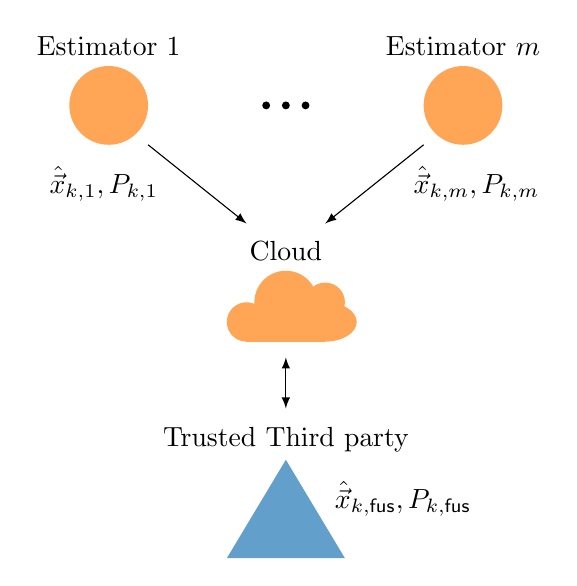
\begin{tikzpicture}
        % Bounding box
        %\draw [gray] (1,-1.5) rectangle (8.5,7);
        % Estimators
        \node at (2.5,6.25) {Estimator $1$};
        \node at (7,6.25) {Estimator $m$};
        \fill [pyplotorange!70] (7,5.5) ellipse (0.5 and 0.5);
        \fill [pyplotorange!70] (2.5,5.5) ellipse (0.5 and 0.5);
        \fill [black] (5,5.5) circle (0.05);
        \fill [black] (4.5,5.5) circle (0.05);
        \fill [black] (4.75,5.5) circle (0.05);
        % Estimates
        \node [right] at (6.25,4.5) {$\hat{\vec{x}}_{k,m},\mat{P}_{k,m}$};
        \node [left] at (3.25,4.5) {$\hat{\vec{x}}_{k,1},\mat{P}_{k,1}$};
        % Fusion
        \node [right] at (5.25,0.5) {$\hat{\vec{x}}_{k,\mathsf{fus}},\mat{P}_{k,\mathsf{fus}}$};
        % Cloud
        \node at (4.75,3.65) {Cloud};
        \fill [pyplotorange!70] (4.75,3) ellipse (0.4 and 0.4);
        \fill [pyplotorange!70] (5.25,2.75) ellipse (0.4 and 0.25);
        \fill [pyplotorange!70] (4.25,2.75) ellipse (0.25 and 0.25);
        \fill [pyplotorange!70] (5.25,3) ellipse (0.25 and 0.25);
        \fill [pyplotorange!70] (4.25,2.5) rectangle (5.25,2.75);
        % Third party
        \node at (4.75,1.25) {Trusted Third party};
        \fill [pyplotblue!70] (5.5,-0.25) -- (4,-0.25) -- (4.75,1);
        % Estimator arrows
        \draw [-latex]  plot coordinates {(3,5)  (4.25,4)};
        \draw [-latex]  plot coordinates {(6.5,5)  (5.25,4)};
        % Third party arrows
        \draw [latex-latex]  plot coordinates {(4.75,2.3)  (4.75,1.65)};
    \end{tikzpicture}
    \label{fig:layout}
\end{figure}

% 
% 888      8888888 88888888888 
% 888        888       888     
% 888        888       888     
% 888        888       888     
% 888        888       888     
% 888        888       888     
% 888        888       888     
% 88888888 8888888     888     
%                              
%                              
%                              
% 
\section{Related Literature}

% 
% 8888888888 888     888  .d8888b. 8888888 .d88888b.  888b    888      888      
% 888        888     888 d88P  Y88b  888  d88P" "Y88b 8888b   888      888      
% 888        888     888 Y88b.       888  888     888 88888b  888      888      
% 8888888    888     888  "Y888b.    888  888     888 888Y88b 888      888      
% 888        888     888     "Y88b.  888  888     888 888 Y88b888      888      
% 888        888     888       "888  888  888     888 888  Y88888      888      
% 888        Y88b. .d88P Y88b  d88P  888  Y88b. .d88P 888   Y8888      888      
% 888         "Y88888P"   "Y8888P" 8888888 "Y88888P"  888    Y888      88888888 
%                                                                               
%                                                                               
%                                                                               
% 
\section{Confidential Cloud Fusion Leaking Fusion Weights}

% 
%  #######           ######  ######## ##    ## 
% ##     ##         ##    ## ##       ###   ## 
%        ##         ##       ##       ####  ## 
%  #######  #######  ######  ######   ## ## ## 
% ##                      ## ##       ##  #### 
% ##                ##    ## ##       ##   ### 
% #########          ######  ######## ##    ## 
% 
\subsection{Two-sensor Secure Fast Covariance Intersection} \label{sec:secfci}
In this section, we will introduce the Secure FCI (SecFCI) fusion algorithm for the two-sensor case, before extending it to the $n$ sensor case in section [sec:multi\_secfci]. The network model we consider is described in section [subsec:problem\_formulation], where sensors are capable of running local estimators, as well as the PHE and ORE encryption schemes from section [sec:encryption]. Each sensor $i$ computes its state estimate $\mean{\vec{x}}_i$ and covariance matrix $\mP_i$ and sends relevant encrypted information to an untrusted cloud fusion center. The querying party is the key holding party and generates the PHE public key $pk$, secret key $sk$, and ORE symmetric key $k$. $pk$ is made available to all parties in the network, and $k$ is made available to the sensors only, via any standard public-key scheme such as RSA [rivestMethodObtainingDigital1978]. When encrypting with ORE key $k$, individual sensors are limited to using only $L$ or $R$ ORE encryption to reduce local information leakage. Thus, consecutive ORE encryptions from any sensor cannot be used to infer local information directly, and can only be compared to encryptions from sensors using the alternate ORE encryption.

From [eqn:ci\_cov\_estimate], we can see that both CI fusion equations can be computed on PHE encryptions of sensor information vectors and information matrices, given valid unencrypted values for each $\omega_i$. For this reason, we allow the leakage of all weights $\omega_i$. Thus, in the two-sensor case, homomorphic fusion is computed by
\begin{equation}
   \mathcal{E}(\mP^{-1}) = \mathcal{E}(\mP^{-1}_1)^{\omega_1}\mathcal{E}(\mP^{-1}_2)^{(1 -\omega_1)} \label{eqn:paillier_ci_cov}
\end{equation}
and
\begin{equation}
   \mathcal{E}(\mP^{-1}\mean{\vec{x}}) = \mathcal{E}(\mP^{-1}_1\mean{\vec{x}}_1)^{\omega_1}\mathcal{E}(\mP^{-1}_2\mean{\vec{x}}_2)^{(1 - \omega_1)}\enspace, \label{eqn:paillier_ci_estimate}
\end{equation}
where we note that $\omega_2=1-\omega_1$ due to the CI requirement [eqn:ci\_omega\_sum\_bound]. We also note that in [eqn:paillier\_ci\_cov] and [eqn:paillier\_ci\_estimate], each resulting value will have exactly one encoding multiplication factor to remove, and can be decoded exactly by using [eqn:qmn\_mult\_decode].
   
All that remains for computing CI homomorphically, in the two-sensor case, is the calculation of parameter $\omega_1$. For this, we approximate the solution to FCI. Since our encoding scheme in section [subsec:encoding] does not allow division, the exact result of [eqn:fci\_2sen\_omega\_sum\_eq] is approximated. This is accomplished by discretizing $\omega_i$ by step-size $s$, such that $s<1$ and $p=1/s \in \mathbb{Z}$, and approximating [eqn:fci\_2sen\_omega\_sum\_eq] with ORE. An ordered discretization of values $\omega^{(x)}$ is defined by
\begin{equation}
   [\omega^{(1)},\dots,\omega^{(p)}] = [0,s,\dots,1-s,1]\enspace,
\end{equation}
and computed by each sensor $i$. Each $\omega^{(x)}$ is multiplied by $\tr(\mP_i)$ and encrypted with ORE key $k$. Sensor $1$'s list is defined by 
\begin{equation}
   [\mathcal{E}^L_{ORE}(\omega^{(1)}\tr(\mP_1)),\dots,\mathcal{E}^L_{ORE}(\omega^{(p)}\tr(\mP_1))]\enspace, \label{eqn:sen1_ore_list}
\end{equation}
and similarly sensor $2$'s by
\begin{equation}
   [\mathcal{E}^R_{ORE}(\omega^{(1)}\tr(\mP_2)),\dots,\mathcal{E}^R_{ORE}(\omega^{(p)}\tr(\mP_2))]\enspace. \label{eqn:sen2_ore_list}
\end{equation}
Note that Sensor $1$ uses only $L$ ORE while sensor $2$ uses only $R$ ORE, and that both lists are ordered. Lists \eqref{eqn:sen1_ore_list} and \eqref{eqn:sen2_ore_list} are sent alongside PHE encryptions of local information vector and information matrix estimates to the fusion center which uses them to estimate the FCI values of $\omega_1$ and $\omega_2$.

From [eqn:fci\_2sen\_omega\_sum\_eq] we know that $\omega_1$ must satisfy
\begin{equation}
   \omega_1 \tr(\mP_1) = (1-\omega_1)\tr(\mP_2)\enspace. \label{eqn:secfci_2sen_intersect}
\end{equation}
If we reverse \eqref{eqn:sen2_ore_list}, we obtain a list equivalent to one with values $\mathcal{E}^R_{ORE}((1-\omega^{(x)})\tr(\mP_2))$ for each discretization step $x$. When the reversed list is decrypted and plotted over \eqref{eqn:sen1_ore_list} the intersection gives the solution to \eqref{eqn:secfci_2sen_intersect} and therefore, \eqref{eqn:fci_2sen_omega_sum_eq}. However, \eqref{eqn:sen1_ore_list} and reversed \eqref{eqn:sen2_ore_list} consist of $L$ and $R$ ORE encryptions respectively, and the intersection must be approximated by locating consecutive $\omega^{(x)}$ discretizations where the sign of comparisons changes. This can be seen in Fig. \ref{fig:2_sensor_sol}, and can be performed in $O(\log{p})$ ORE comparisons using a binary search.
\begin{figure}[tb]
   \begin{center}
      \includegraphics{figures/2_sensors.pdf}
   \end{center}
   \caption{Approximation of $\omega_1$ with discretization step-size $s=0.1$. Only comparisons between line points are used.}
   \label{fig:2_sensor_sol}
\end{figure}
Consecutive $\omega^{(x)}$ and $\omega^{(x+1)}$ for which list comparisons differ can be used to estimate the true intersection, and $\omega_1$, by
\begin{equation}
   \omega_1 \approx 0.5(\omega^{(x)} + \omega^{(x+1)})\enspace. \label{eqn:secfci_2sen_omega}
\end{equation}
In the case a comparison returns equality, the exact value of $\omega^{(x)}$ can be taken to be $\omega_1$.

The fusion center can then use its values for $\omega_1$ and $\omega_2 = 1-\omega_1$ and the received PHE encryptions of local information vectors and information matrices to compute \eqref{eqn:paillier_ci_cov} and \eqref{eqn:paillier_ci_estimate}.

% 
% ##    ##          ######  ######## ##    ## 
% ###   ##         ##    ## ##       ###   ## 
% ####  ##         ##       ##       ####  ## 
% ## ## ## #######  ######  ######   ## ## ## 
% ##  ####               ## ##       ##  #### 
% ##   ###         ##    ## ##       ##   ### 
% ##    ##          ######  ######## ##    ## 
% 
\subsection{Multi-sensor Secure Fast Covariance Intersection} \label{sec:multi_secfci}
When computing the SecFCI fusion for $n$ sensors, we solve \eqref{eqn:ci_cov_estimate} homomorphically by computing
\begin{equation}
   \mathcal{E}(\mP^{-1}) = \mathcal{E}(\mP^{-1}_1)^{\omega_1}\cdots\mathcal{E}(\mP^{-1}_n)^{\omega_n} \label{eqn:n_sen_paillier_ci_cov}
\end{equation}
and
\begin{equation}
   \mathcal{E}(\mP^{-1}\mean{\vec{x}}) = \mathcal{E}(\mP^{-1}_1\mean{\vec{x}}_1)^{\omega_1}\cdots\mathcal{E}(\mP^{-1}_n\mean{\vec{x}}_n)^{\omega_n}\enspace. \label{eqn:n_sen_paillier_ci_estimate}
\end{equation}
As with the two-sensor case, encoded results from \eqref{eqn:n_sen_paillier_ci_cov} and \eqref{eqn:n_sen_paillier_ci_estimate} contain exactly one multiplication factor to remove and can be decoded exactly with [eqn:qmn\_mult\_decode]. Again we are just left with the task of computing the plaintext weights $\omega_1,\dots,\omega_n$.

Our approach to the $n$ sensor case is to solve all $n-1$ conditions in \eqref{eqn:fci_eq} using the two-sensor method, and combining partial solutions to compute the final result. When we consider a Euclidean dimension for each $\omega_i$, partial solutions can be considered geometrically as hyperplanes of $n-2$ dimension, over the $n-1$ dimensional solution space given by \eqref{eqn:ci_omega_sum_bound}. 

This can be visualized in the three sensor case, which requires solving partial solutions
\begin{equation}
   \omega_1 \tr(\mP_1) - \omega_2 \tr(\mP_2) = 0,\ \omega_1+\omega_2=1-\omega_3 \label{eqn:3_sensor_partial_sol_1}
\end{equation}
and
\begin{equation}
   \omega_2 \tr(\mP_2) - \omega_3 \tr(\mP_3) = 0,\ \omega_2+\omega_3=1-\omega_1\enspace. \label{eqn:3_sensor_partial_sol_2}
\end{equation}
We can use the two-sensor method from section \ref{sec:secfci} to solve \eqref{eqn:3_sensor_partial_sol_1} exactly when $\omega_3=0$, and know that when $\omega_3=1$, then $\omega_1=\omega_2=0$. These two points are enough to define the two-dimensional partial solution \eqref{eqn:3_sensor_partial_sol_1} which can be seen plotted over the possible solution space in Fig. \ref{fig:3_sensor_partial_sol}. Fig. \ref{fig:3_sensor_partial_sols} shows both partial solutions \eqref{eqn:3_sensor_partial_sol_1} and \eqref{eqn:3_sensor_partial_sol_2} plotted over the solution space.
\begin{figure*}[tb]
   \begin{subfigure}[t]{0.3\textwidth}
      \begin{center}
         \includegraphics{figures/partial_sol1.pdf}
      \end{center}
      \caption{Partial solution to \eqref{eqn:3_sensor_partial_sol_1}.}
      \label{fig:3_sensor_partial_sol}
   \end{subfigure}
   ~
   \begin{subfigure}[t]{0.3\textwidth}
      \begin{center}
         \includegraphics{figures/partial_sols.pdf}
      \end{center}
      \caption{Partial solutions to \eqref{eqn:3_sensor_partial_sol_1} and \eqref{eqn:3_sensor_partial_sol_2}.}
      \label{fig:3_sensor_partial_sols}
   \end{subfigure}
   ~
   \begin{subfigure}[t]{0.3\textwidth}
      \begin{center}
         \includegraphics{figures/partial_sol_planes.pdf}
      \end{center}
      \caption{Partial solutions as planes.}
      \label{fig:3sen_planes}
   \end{subfigure}
   \caption{Partial solutions over $\omega_1$, $\omega_2$, and $\omega_3$ solution space.}
   \label{fig:partial_sols_and_planes}
\end{figure*}
The final solution from all partial solutions is computed by finding their intersection. This can be seen in Fig. \ref{fig:3_sensor_partial_sols} as the intersection of the $(\omega_1,\omega_2)$ and $(\omega_2,\omega_3)$ partial solution lines.

To simplify computing the partial solution intersection, we define equivalent planes for each of the partial solutions, perpendicular to the solution space, in the form
\begin{equation}
   a_1\omega_1 + a_2\omega_2 +a_3\omega_3 + a_4 = 0\enspace, \label{eqn:3sen_plane_eq}
\end{equation}
and solve the resulting linear system for finding the intersection of all planes and the solution space. This is given by
\begin{equation}
   \begin{bmatrix}
      a_1^{(1)} & a_2^{(1)} & a_3^{(1)} \\
      a_1^{(2)} & a_2^{(2)} & a_3^{(2)} \\
      1 & 1 & 1
   \end{bmatrix}
   \begin{bmatrix}
      \omega_1 \\
      \omega_2 \\
      \omega_3
   \end{bmatrix}
   =
   \begin{bmatrix}
      a_3^{(1)} \\
      a_4^{(2)} \\
      1
   \end{bmatrix}\enspace, \label{eqn:3sen_plane_sol_eq}
\end{equation}
where $a_i^{(j)}$ denotes parameter $i$ of partial solution $j$, and has been shown visually in Fig. \ref{fig:3sen_planes}.

In the $n$ sensor case, we can similarly solve partial solutions by first using the method from section \ref{sec:secfci} to solve equations with two parameters $\omega_k$ and $\omega_{k+1}$ when letting all $\omega_i=0,\ i\neq k,k+1$. For each equation we can then compute remaining partial solution points at $\omega_i=1,\ i\neq k,k+1$ with $\omega_j=0,\ j\neq i$. Perpendicular hyperplanes can then be similarly defined in the form 
\begin{equation}
   a_1\omega_1 + \dots +a_n\omega_n + a_{n+1} = 0\enspace. \label{eqn:nsen_plane_eq}
\end{equation}
Due to their inherent orthogonality, and that all meaningful covariance traces are strictly positive, the $n-1$ partial solution hyperplanes are guaranteed to intersect at exactly one point. The hyperplane intersection results in the linear system 
\begin{equation}
   \begingroup
   \setlength\arraycolsep{2pt}
   \begin{bmatrix}
      a_1^{(1)} & a_2^{(1)} & \cdots & a_{n}^{(1)} \\
      \vdots & \vdots & \ddots & \vdots \\
      a_1^{(n-1)} & a_2^{(n-1)} & \cdots & a_{n}^{(n-1)} \\
      1 & 1 & \cdots & 1
   \end{bmatrix}
   \begin{bmatrix}
      \omega_1 \\
      \vdots \\
      \omega_{n-1} \\
      \omega_{n}
   \end{bmatrix}
   \!=\!
   \begin{bmatrix}
      a_{n+1}^{(1)} \\
      \vdots \\
      a_{n+1}^{(n-1)} \\
      1
   \end{bmatrix}\enspace, \label{eqn:hyperplane_sol_eq}
   \endgroup
\end{equation}
and gives the solution to the SecFCI $\omega_i$ weights.

As all $O(n\log{p})$ ORE comparisons are done between sequential sensors $i$ and $i+1$, $L$ and $R$ ORE encryptions can be used to the same effect as for the two-sensor case. The ORE ordered list sent from each sensor $i$ is given by
\begin{equation}
   \begin{aligned} \label{eqn:sensor_lists}
      &[\mathcal{E}^L_{ORE}(\omega^{(1)}\tr(\mP_i)),\dots,\mathcal{E}^L_{ORE}(\omega^{(p)}\tr(\mP_i))],\,i\text{ odd} \\
      &[\mathcal{E}^R_{ORE}(\omega^{(1)}\tr(\mP_i)),\dots,\mathcal{E}^R_{ORE}(\omega^{(p)}\tr(\mP_i))],\,i\text{ even}.
   \end{aligned}
\end{equation}
When combining \eqref{eqn:sensor_lists} with PHE encryptions of local information vectors and information matrices, SecFCI can be computed entirely homomorphically by \eqref{eqn:n_sen_paillier_ci_cov} and \eqref{eqn:n_sen_paillier_ci_estimate}.

Briefly considering the security of our scheme, we note that any leaked information from ORE lists \eqref{eqn:sensor_lists}, as described in [chenettePracticalOrderRevealingEncryption2016], can be considered a subset of knowing the estimated fusion weights $\omega_1,\dots,\omega_n$, which specify relative sizes of sensor covariance traces, and we already consider public. Thus only IND-CPA and IND-OCPA (after accounting for leakage through public weights) encryptions are made available to the fusion centre.

% 
%  ######   #######  ##     ## ########  
% ##    ## ##     ## ###   ### ##     ## 
% ##       ##     ## #### #### ##     ## 
% ##       ##     ## ## ### ## ########  
% ##       ##     ## ##     ## ##        
% ##    ## ##     ## ##     ## ##        
%  ######   #######  ##     ## ##        
% 
\subsection{Computational Complexity} \label{subsec:complexity}
Given the state estimates and estimate errors at each sensor, we wish to show the computational complexity of the SecFCI algorithm for the $n$ sensor case. We will assume that both Lewi ORE and Paillier PHE schemes use the same length security parameter (and equivalently key size), such that $\lambda_{Lewi} = \lambda_{Paillier} = \log{N}$, where $\lambda_{s}$ represents encryption scheme $s$'s security parameter, and $N$ the Paillier modulus and encryptable integer limit. We also note the distinction between floating-point or small integer operations, which are typically treated as having $O(1)$ runtime, and large integer operations whose complexities are dependent on bit length. While architectures exist for speeding up encryption operations [gueronIntelAdvancedEncryption2010], we consider software implementations and treat large integer operations in terms of bit operations explicitly.

From [paillierPublicKeyCryptosystemsBased1999,lewiOrderRevealingEncryptionNew2016], and the assumptions made above, we have summarized the operation complexities of the two schemes in Table \ref{tab:complex_ops}.
\begin{table}[tb]
   \centering
   \caption{Computation complexity of encryption operations.}
   \label{tab:complex_ops}
   \begin{tabular}{ |c|c| }
      \hline
      \textbf{Operation} & \textbf{Complexity} \\ 
      \hline
      Paillier enc. & $O(\log^3{N})$ \\ 
      Paillier dec. & $O(\log^3{N})$ \\ 
      Paillier add. & $O(\log^2{N})$ \\ 
      Paillier scalar mult. & $O(\log^3{N})$ \\ 
      Lewi $L$ enc. & $O(\log^2{N})$ \\ 
      Lewi $R$ enc. & $O(\log^2{N})$ \\ 
      Lewi comp. & $O(\log^2{N})$ \\ 
      \hline
   \end{tabular}
\end{table}
In contrast to some current FHE schemes, these operations are of a much lower complexity than [vandijkFullyHomomorphicEncryption2010a], which has complexity $O(\lambda^{10})$ for integer operations, and [stehleFasterFullyHomomorphic2010], which computes single bit operations in $O(\lambda^{3.5})$ adding significant overhead for integer arithmetic.

Finally, applying the operations from Table \ref{tab:complex_ops} to the SecFCI algorithm, we summarize the total complexity of SecFCI at the sensors and the fusion centre in Table \ref{tab:complex}, with the unencrypted complexities of FCI shown for reference. 
\begin{table}[tb]
   \centering
   \caption{Computation complexity at sensors and fusion centre.}
   \label{tab:complex}
   \begin{tabular}{ |c|c|c| }
      \hline
       & \textbf{FCI} & \textbf{SecFCI} \\ 
      \hline
      Sensors & $O(1)$ & $O\left(p\log^2{N} + \log^3{N}\right)$ \\ 
      Fusion & $O(n^3)$ & $O\left(n\log{p}\log^2{N} + n\log^3{N} + n^3\right)$ \\ 
      \hline
   \end{tabular}
\end{table}

% 
%  ######  #### ##     ## 
% ##    ##  ##  ###   ### 
% ##        ##  #### #### 
%  ######   ##  ## ### ## 
%       ##  ##  ##     ## 
% ##    ##  ##  ##     ## 
%  ######  #### ##     ## 
% 
\subsection{Simulation Results} \label{sec:results}
We have implemented a simulation to demonstrate the accuracy of SecFCI approximating FCI. Three sensors independently measure a constant-speed linear process and simultaneously run a Kalman filter on their measurements. Estimates are sent both encrypted and unencrypted to a fusion centre that computes the SecFCI and FCI fusions on the received data respectively. Encrypted estimates are comprised of PHE encryptions of the information vector and information matrix, $\mathcal{E}(\mP^{-1}_i\mean{\vec{x}}_i)$ and $\mathcal{E}(\mP^{-1}_i)$, in addition to the ORE list given by \eqref{eqn:sensor_lists} with discretization step $s=0.1$. Unencrypted estimates consist of the state estimate $\mean{\vec{x}}_i$ and covariance $\mP_i$. The trajectory and fused estimates are shown in Fig. \ref{fig:fci_secfci_traj}.
\begin{figure}[tb]
   \begin{center}
      \includegraphics{figures/fci_secfci_cmp.pdf}
   \end{center}
   \caption{Tracking simulation comparing SecFCI and FCI.}
   \label{fig:fci_secfci_traj}
\end{figure}

To derive an upper bound on the accuracy difference between SecFCI and FCI, we note the two factors which introduce inconsistency between the two methods: the encoding method from section \ref{subsec:complexity}, and the difference in fusion weights. Due to the possibility of choosing sufficiently large integer and fractional bit lengths $i$ and $f$, we will only consider the error caused by the difference in weights. We will treat this error as the distance between respective weight vectors
\begin{equation}
   \begin{aligned}
      &\vec{\omega}_{SecFCI} = (\omega_{1,SecFCI},\dots,\omega_{n,SecFCI}) \\
      &\vec{\omega}_{FCI} = (\omega_{1,FCI},\dots,\omega_{n,FCI})\enspace,
   \end{aligned}
\end{equation}
where $\omega_{i,s}$ denotes weight $\omega_i$ from algorithm $s$. From section \ref{sec:secfci} we see that the largest difference $|\omega_{i,FCI} - \omega_{i,SecFCI}|$ is strictly bounded by $s/2$. As shown in section \ref{sec:multi_secfci}, when more sensors are involved, a tighter bound on this difference is dependent on the value of $\vec{\omega}_{i,FCI}$, but will remain strictly bounded by $s/2$. Therefore, we can give a strict upper bound on the distance between weight vectors as
\begin{equation}
   |\vec{\omega}_{FCI} - \vec{\omega}_{SecFCI}| < 0.5\sqrt{ns^2}\enspace. \label{eqn:accuracy_error_bound}
\end{equation}

Finally, components of $\omega_{i,SecFCI}$, $\omega_{i,FCI}$ and the errors $|\vec{\omega}_{FCI} - \vec{\omega}_{SecFCI}|$, have been plotted over time in Fig. \ref{fig:fci_secfci_omegas}, and show the computed error bound when $n=3$ and $s=0.1$.
\begin{figure}[tb]
   \begin{center}
      \includegraphics{figures/omegas_cmp.pdf}
   \end{center}
   \caption{$\vec{\omega}_{SecFCI}$ and $\vec{\omega}_{FCI}$ components.}
   \label{fig:fci_secfci_omegas}
\end{figure}

% 
% 8888888888 888     888  .d8888b. 8888888 .d88888b.  888b    888      888b    888 888      
% 888        888     888 d88P  Y88b  888  d88P" "Y88b 8888b   888      8888b   888 888      
% 888        888     888 Y88b.       888  888     888 88888b  888      88888b  888 888      
% 8888888    888     888  "Y888b.    888  888     888 888Y88b 888      888Y88b 888 888      
% 888        888     888     "Y88b.  888  888     888 888 Y88b888      888 Y88b888 888      
% 888        888     888       "888  888  888     888 888  Y88888      888  Y88888 888      
% 888        Y88b. .d88P Y88b  d88P  888  Y88b. .d88P 888   Y8888      888   Y8888 888      
% 888         "Y88888P"   "Y8888P" 8888888 "Y88888P"  888    Y888      888    Y888 88888888 
%                                                                                           
%                                                                                           
%                                                                                           
% 
\section{Confidential Cloud Fusion Without Leakage}

With the problem and preliminaries introduced, we can now present our encrypted FCI method that leaks no estimator information to the fusing cloud. The core idea behind the method is to postpone the evaluation of operations that cannot be performed homomorphically until partial results are queried and decrypted by the key-holding third party. The remaining operations can then be evaluated on unencrypted inputs to produce the correct results.

First, we note that the FCI fusion equations [eqn:ci\_cov\_fusion] and [eqn:ci\_est\_fusion] can be rearranged and substituted with weights [eqn:fci\_weights] to obtain the equations
\begin{equation}\label{eqn:fci_cov_rearrange}
    \mat{P}_{k,\mathsf{fus}} = \left(\left(\sum_{i=1}^m \frac{1}{\tr(\mat{P}_{k,i})}\right)^{-1}\sum_{i=1}^m \frac{1}{\tr(\mat{P}_{k,i})}\mat{P}_{k,i}^{-1}\right)^{-1}
\end{equation}
and
\begin{equation}\label{eqn:fci_est_rearrange}
    \hat{\vec{x}}_{k,\mathsf{fus}} = \mat{P}_{k,\mathsf{fus}}\left(\sum_{i=1}^m \frac{1}{\tr(\mat{P}_{k,i})}\right)^{-1}\sum_{i=1}^m\frac{1}{\tr(\mat{P}_{k,i})}\mat{P}_{k,i}^{-1}\hat{\vec{x}}_{k,i}\,.
\end{equation}
In this form, innermost summations  
\begin{equation}
    \begin{split}
        \sum_{i=1}^m \frac{1}{\tr(\mat{P}_{k,i})}\,,\ \sum_{i=1}^m &\frac{1}{\tr(\mat{P}_{k,i})}\mat{P}_{k,i}^{-1}\text{ and }\\ 
        &\qquad\sum_{i=1}^m\frac{1}{\tr(\mat{P}_{k,i})}\mat{P}_{k,i}^{-1}\hat{\vec{x}}_{k,i}
    \end{split}
\end{equation}
combine information from individual estimators $i$ and are computable homomorphically given suitable encryptions. Encryptions of these sums can then be decrypted by the key-holding third party, before remaining inversions and multiplications in \eqref{eqn:fci_cov_rearrange} and \eqref{eqn:fci_est_rearrange} can be computed to obtain the final results. To depict this process, pseudocode for the encryption at estimators, fusion at the cloud and decryption by the third party are provided in algorithms~\ref{alg:est_enc}, \ref{alg:cloud_fus} and \ref{alg:fus_query}, respectively.
\begin{algorithm}[htbp]
\caption{Estimator Encryption}\label{alg:est_enc}
\begin{algorithmic}[1]
    \setstretch{1.35}
    \Procedure{Estimate}{$i$, $k$, $\mathsf{pk}$, $\phi$}
    \State Estimate $\hat{\vec{x}}_{k,i}$ locally
    \State Estimate $\mat{P}_{k,i}$ locally
    \LineComment{Public key is encoding and encryption modulus}
    \State $N \gets \mathsf{pk}$
    \LineComment{Encode scaling, covariance and estimate components}
    \State $\tilde{s}_{k,i} \gets \mathsf{E}_{N,\phi}\left(\frac{1}{\tr(\mat{P}_{k,i})}\right)$
    \State $\tilde{\mat{C}}_{k,i} \gets \mathsf{E}_{N,\phi}\left(\frac{1}{\tr(\mat{P}_{k,i})}\mat{P}_{k,i}^{-1}\right)$
    \State $\tilde{\vec{e}}_{k,i} \gets \mathsf{E}_{N,\phi}\left(\frac{1}{\tr(\mat{P}_{k,i})}\mat{P}_{k,i}^{-1}\hat{\vec{x}}_{k,i}\right)$
    \LineComment{Encrypt scaling, covariance and estimate components}
    \State $s_{k,i} \gets \mathcal{E}_{\mathsf{pk}}\left(\tilde{s}_{k,i}\right)$
    \State $\mat{C}_{k,i} \gets \mathcal{E}_{\mathsf{pk}}\left(\tilde{\mat{C}}_{k,i}\right)$
    \State $\vec{e}_{k,i} \gets \mathcal{E}_{\mathsf{pk}}\left(\tilde{\vec{e}}_{k,i}\right)$
    \State Send $s_{k,i}$, $\mat{C}_{k,i}$ and $\vec{e}_{k,i}$ to fusing cloud
    \EndProcedure
\end{algorithmic}
\end{algorithm}
\begin{algorithm}[htbp]
\caption{Cloud Fusion}\label{alg:cloud_fus}
\begin{algorithmic}[1]
    \setstretch{1.35}
    \Procedure{Fuse}{$k$, $\mathsf{pk}$}
    \State Receive $s_{k,i}$, $\mat{C}_{k,i}$ and $\vec{e}_{k,i}$ for all $1\leq i \leq m$
    \State $N \gets \mathsf{pk}$
    \State $s_k \gets \prod_{i=1}^{m} s_{k,i} \pmod{N^2}$
    \State $\mat{C}_k \gets \otimes_{i=1}^{m} \mat{C}_{k,i} \pmod{N^2}$
    \State $\vec{e}_k \gets \otimes_{i=1}^{m} \vec{e}_{k,i} \pmod{N^2}$
    \State Store $s_k$, $\mat{C}_k$ and $\vec{e}_k$ in case of query
    \EndProcedure
\end{algorithmic}
\end{algorithm}
\begin{algorithm}[htbp]
\caption{Fusion Query}\label{alg:fus_query}
\begin{algorithmic}[1]
    \setstretch{1.35}
    \Procedure{GetResult}{$k$, $\mathsf{pk}$, $\mathsf{sk}$, $\phi$}
    \State Query and receive $s_k$, $\mat{C}_k$ and $\vec{e}_k$ from fusing cloud
    \State $N \gets \mathsf{pk}$
    \LineComment Decrypt
    \State $\tilde{s}_k \gets \mathcal{D}_{\mathsf{sk}}\left(s_k\right)$
    \State $\tilde{\mat{C}}_k \gets \mathcal{D}_{\mathsf{sk}}\left(\mat{C}_k\right)$
    \State $\tilde{\vec{e}}_k \gets \mathcal{D}_{\mathsf{sk}}\left(\vec{e}_k\right)$
    \LineComment Decode
    \State $\bar{s}_k \gets \mathsf{E}^{-1}_{N,\phi}\left(\tilde{s}_k\right)$
    \State $\bar{\mat{C}}_k \gets \mathsf{E}^{-1}_{N,\phi}\left(\tilde{\mat{C}}_k\right)$
    \State $\bar{\vec{e}}_k \gets \mathsf{E}^{-1}_{N,\phi}\left(\tilde{\vec{e}}_k\right)$
    \LineComment Compute Fusion
    \State $\mat{P}_{k,\mathsf{fus}} \gets \left(\bar{s}_k^{-1} \cdot \bar{\mat{C}}_k\right)^{-1}$
    \State $\hat{\vec{x}}_{k,\mathsf{fus}} \gets \mat{P}_{k,\mathsf{fus}} \cdot \bar{s}_k^{-1} \cdot \bar{\vec{e}}_k$
    \State \Return $\hat{\vec{x}}_{k,\mathsf{fus}}$, $\mat{P}_{k,\mathsf{fus}}$
    \EndProcedure
\end{algorithmic}
\end{algorithm}

\begin{remark}\label{rem:seq_extension}
    Along with allowing the summations to be performed homomorphically on the cloud, we note that this form of the FCI also allows the cloud's partial fusion operations to be evaluated sequentially. This can be seen in algorithm~\ref{alg:cloud_fus}, where individual components $s_{k,i}$, $\mat{C}_{k,i}$ and $\vec{e}_{k,i}$ from each estimator can continue to be aggregated as additional estimators send their estimate information. This, in turn, supports the dynamic joining and leaving of estimators in the network without affecting the cloud or the operations of a trusted third party. The security implications of such an extension are discussed further in section~\ref{subsec:security}.
\end{remark}

% 
%  ######   #######  ##     ## ########  
% ##    ## ##     ## ###   ### ##     ## 
% ##       ##     ## #### #### ##     ## 
% ##       ##     ## ## ### ## ########  
% ##       ##     ## ##     ## ##        
% ##    ## ##     ## ##     ## ##        
%  ######   #######  ##     ## ##        
% 
\section{Complexity}\label{sec:complexity}
The method described provides a level of security when relying on an untrusted cloud for fusing estimates. However, the added reliance on an encryption scheme and the additional computations at the third party intuitively increase the computational complexity of the algorithm and the required capabilities of participating parties. Here, we present the complexity of operations during fusion, required by each party at every timestep $k$. We assume encoding and decoding operations have complexity $O(1)$ (due to their comparative insignificance when compared to associated encryption and decryption operations) and use \cite{paillierPublicKeyCryptosystemsBased1999} to obtain the encryption complexities of the Paillier encryption scheme in table \ref{tab:enc_cmplx}, with security parameter $\lambda = \log{N}$.
\begin{table}[tb]
    \centering
    \caption{Computation complexity of encryption operations.}
    \label{tab:enc_cmplx}
    \begin{tabular}{|c|c|}
       \hline
       \textbf{Operation} & \textbf{Complexity} \\ 
       \hline
       Encryption & $O(\log^3{N})$ \\ 
       Decryption & $O(\log^3{N})$ \\ 
       Addition & $O(\log^2{N})$ \\ 
       Scalar mult. & $O(\log^3{N})$ \\ 
       \hline
    \end{tabular}
 \end{table}
In table \ref{tab:fus_cmplx}, we compare the complexities of the unencrypted FCI algorithm and the method presented in this work.
\begin{table}[tb]
    \centering
    \caption{Computation complexity at parties during fusion.}
    \label{tab:fus_cmplx}
    \begin{tabular}{ |c|c|c| }
       \hline
        & \textbf{FCI} & \textbf{Our Method} \\ 
       \hline
       Estimator & $O(1)$ & $O\left(n^2\log^3{N}\right)$ \\ 
       Fusion & $O(mn^3)$ & $O\left(mn^2\log^2{N}\right)$ \\ 
       Third party & $O(1)$ & $O\left(n^2\log^3{N} + n^3\right)$ \\ 
       \hline
    \end{tabular}
 \end{table}
It can be seen that the burden of computation is greatly increased at the estimators and the third party, in particular when dimension $n$ is large and when a long encryption key $N$ is used. Naturally, an application of the proposed method would need to consider these requirements in terms of computation time and required hardware.

\subsection{Security Analysis}\label{subsec:security}
The provable security of the presented method is relatively straightforward. Our aim for IND-CPA security of all information received by the cloud, sent by the estimators or observable by eavesdroppers is achieved by the homomorphic Paillier encryption scheme. Since all transmitted information is encrypted and the cloud, estimators and eavesdroppers do not hold the secret key $\mathsf{sk}$, IND-CPA is met at all parties.

We note, however, an implicit assumption made when encrypting multidimensional data element-wise. While individual elements are indistinguishable, element-wise encryption does not encrypt the estimate's dimension $n$, which remains implicitly public. While existing methods allow the complete homomorphic encryption of vectors [alexandruPrivateWeightedSum2020], they are left for future work and considered beyond the scope of this work. Instead, we acknowledge the implicit leakage of $n$ and note that, while this may leak information about the fusion's use case, state estimates remain hidden. Additionally, intuitive extensions to the scheme, such as the dynamic joining and leaving of estimators in remark \ref{rem:seq_extension}, may introduce further implicit leakages that must be considered if security is analysed. In this example, the periodic estimation may leak to the cloud when estimators are within an estimation range or context, and a solution may be sending dummy measurements with $s_{k,i}=\mathcal{E}_{\mathsf{pk}}(\mathsf{E}_{N,\phi}(0))$ when estimator $i$ is out of range. This extension is presented only as an example of when care needs to be taken to maintain desired security goals, but in general, extensions and solutions are task-dependent and not a focus of this work.


% 
%  ######  #### ##     ## 
% ##    ##  ##  ###   ### 
% ##        ##  #### #### 
%  ######   ##  ## ### ## 
%       ##  ##  ##     ## 
% ##    ##  ##  ##     ## 
%  ######  #### ##     ## 
% 
\subsection{Simulation}\label{sec:simulation}
Fusion estimates and error covariances from the proposed encrypted FCI method differ from unencrypted FCI only when quantisation errors are large or summation overflows occur. As stated in section [subsec:encoding], when the Paillier modulus $N$ is large, these errors can often be considered negligible. In this section, we demonstrate this similarity in performance between the encrypted and unencrypted FCI fusion algorithms with a simulation. Code was written in the Python programming language, using the $\mathsf{phe}$ Paillier encryption scheme library [PythonPaillier2013] and a $512$ bit length key (bit length of $N$). The simulation implements a linear constant velocity model,
\begin{equation}\label{eqn:sim_sys_model}
    \vec{x}_k =
    \begin{bmatrix}
        1 & 0.5 & 0 & 0\\
        0 & 1 & 0 & 0\\
        0 & 0 & 1 & 0.5\\
        0 & 0 & 0 & 0
    \end{bmatrix}
    \cdot \vec{x}_{k-1} + \vec{w}_k\,,
\end{equation}
with noise term $\vec{w}_k \sim \mathcal{N}(\vec{0}, \mat{Q})$ and
\begin{equation}
    \mat{Q} = 10^{-3} \cdot
    \begin{bmatrix}
        0.42 & 1.25 & 0 & 0\\
        1.25 & 5 & 0 & 0\\
        0 & 0 & 0.42 & 1.25\\
        0 & 0 & 1.25 & 5
    \end{bmatrix}\,.
\end{equation}
At each timestep $k$, the system state $\vec{x}_k$ is estimated by $m=4$ estimators, $1\leq i \leq 4$, using a standard linear Kalman filter (KF) [haugBayesianEstimationTracking2012] and producing estimates and error covariances $\hat{\vec{x}}_{k,i}$ and $\mat{P}_{k,i}$, respectively. The measurements used by the KF, $\vec{z}_{k,i}$, follow the measurement models
\begin{equation}
    \vec{z}_{k,i} = 
    \begin{bmatrix}
        1 & 0 & 0 & 0\\
        0 & 0 & 1 & 0
    \end{bmatrix}
    \cdot \vec{x}_k + \vec{v}_{k,i}\,,
\end{equation}
with noise terms $\vec{v}_{k,i} \sim \mathcal{N}(\vec{0}, \mat{R}_i)$ and covariances sampled indepedently, resulting in
\begin{equation}
    \begin{split}
        &\mat{R}_1 = 
        \begin{bmatrix}
            4.77 & -0.15\\
            -0.15 & 4.94
        \end{bmatrix}\,,\ 
        \mat{R}_2 = 
        \begin{bmatrix}
            2.99 & -0.55\\
            -0.55 & 4.44
        \end{bmatrix}\,,\\
        &\mat{R}_3 = 
        \begin{bmatrix}
            2.06 & 0.68\\
            0.68 & 1.96
        \end{bmatrix}\text{ and }
        \mat{R}_4 = 
        \begin{bmatrix}
            1.17 & 0.80\\
            0.80 & 0.64
        \end{bmatrix}\,.
    \end{split}
\end{equation}
The fusion results of $1000$ simulation runs are shown in figure \ref{fig:sim_error_plot}. 
\begin{figure}[htbp]
    \centering
    \includegraphics{figures/sim_error_plot.pdf}
    \caption{Average RMSE of encrypted and unencrypted FCI fusion over $1000$ simulations.}
    \label{fig:sim_error_plot}
\end{figure}
From the figure, we can see the expected similarity in performance between the encrypted and unencrypted FCI methods. Additionally, we note that the current recommended key length for the Paillier encryption scheme is $2048$ bits [barkerRecommendationPairWiseKey2019], easily supporting a modulus $N$ and fractional precision $\phi$ that guarantee similar performance.






% 
%  .d8888b.   .d88888b.  888b    888  .d8888b.  
% d88P  Y88b d88P" "Y88b 8888b   888 d88P  Y88b 
% 888    888 888     888 88888b  888 888    888 
% 888        888     888 888Y88b 888 888        
% 888        888     888 888 Y88b888 888        
% 888    888 888     888 888  Y88888 888    888 
% Y88b  d88P Y88b. .d88P 888   Y8888 Y88b  d88P 
%  "Y8888P"   "Y88888P"  888    Y888  "Y8888P"  
%                                               
%                                               
%                                               
% 
\section{Conclusions}

%FCI is a commonly used, and efficiently computable, approximation to the CI optimization problem that requires the sharing of local sensor estimates to compute their fusion. We propose a secure approximation to FCI, SecFCI, to compute the fused estimate homomorphically. The novel encrypted fusion approach may find uses in various security-critical applications or over untrusted networks subject to eavesdroppers and malicious participants. Possible future work includes run-time comparisons with FHE implementations, giving a computational bound for its practicality, and quantification of fusion weight leakages via formal security proofs.

%In this work, we have presented a method for computing encrypted Fast Covariance Intersection homomorphically on an untrusted cloud and discussed its security guarantees. The method ensures no estimator information leakage at the cloud, eavesdroppers or other estimators and an accompanying simulation demonstrates its minimal effect on estimation performance when compared to the unencrypted algorithm. Applications include a variety of distributed fusion tasks when external fusing computations are required such as weather forecasting and vehicle localisation. Future work on the topic aims to extend the method to include multivariable encryption, hiding the dimension variable $n$, and generalising to decentralised environments where individual fusing parties are untrusted.

\chapter{Distributed Non-Linear Measurement Fusion with Untrusted Participants}


\section{Problem Formulation}
In this work, we consider the context of privacy-preserving range sensor navigation, where we want no sensor to learn any information about the navigator or other sensors beyond their local measurements, and the navigator not to learn any information about individual sensors beyond its location estimate. The problem is two-fold, in that we require explicit cryptographic requirements with a suitable encryption scheme meeting them as well as an estimation scheme that can use the encryption in the context of range-only navigation.

To give a formal cryptographic requirement in a distributed setting, we must first consider the communication requirements of our context and define the attacker capabilities and the desired security of a suitable encryption scheme. In this section, we will define a communication protocol and the relevant formal definition of security we aim to achieve, followed by the estimation problem to which we will apply it.

% 
%  ######  ########  ##    ## ########  ########  #######     ########  ########   #######  ########  
% ##    ## ##     ##  ##  ##  ##     ##    ##    ##     ##    ##     ## ##     ## ##     ## ##     ## 
% ##       ##     ##   ####   ##     ##    ##    ##     ##    ##     ## ##     ## ##     ## ##     ## 
% ##       ########     ##    ########     ##    ##     ##    ########  ########  ##     ## ########  
% ##       ##   ##      ##    ##           ##    ##     ##    ##        ##   ##   ##     ## ##     ## 
% ##    ## ##    ##     ##    ##           ##    ##     ##    ##        ##    ##  ##     ## ##     ## 
%  ######  ##     ##    ##    ##           ##     #######     ##        ##     ##  #######  ########  
% 

\subsection{Formal Cryptographic Problem} \label{subsec:crypto_problem}
The communication between the navigator and sensors in our estimation problem will be decomposed into a simple two-step bi-directional protocol that will simplify defining formal security. In section \ref{sec:priv_localisation}, we will show how this protocol is sufficient to compute the location estimate at a navigator while meeting our desired privacy goals. The communication protocol is as follows.

At every \textit{instance} $t$ (used to distinguish from an estimation \textit{timestep}), the navigator first broadcasts $m$ weights $\omega_j^{(t)}, j\in\{1,\dots,m\}$ to all sensors $i\in\{1,\dots,n\}$, who individually compute linear combinations $l^{(t)}_i=\sum^m_{j=1}a_{j,i}^{(t)}\omega_i^{(t)}$ based on their measurement data $a_{j,i}$. Linear combinations are then sent back to the navigator, who computes their sum $\sum^n_{i=1}l^{(t)}_{i}$. This two-step linear combination aggregation protocol has been visually displayed in figure \ref{fig:agg_steps}.
\begin{figure}[htbp]
\centering
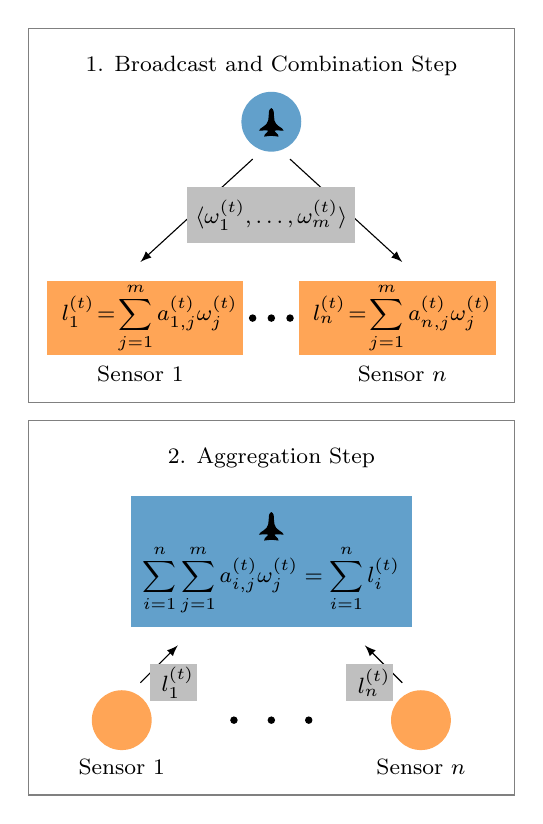
\begin{tikzpicture}[font=\footnotesize,scale=0.95]
    % Step 1
    \node at (3.25,5.5) {1. Broadcast and Combination Step};
    % Navigator
    \fill (3.25,4.75) [pyplotblue!70] ellipse (0.4 and 0.4);
    \pic[xscale=0.22,yscale=0.3] at (3.25,4.9225) {plane};
    % Sensors
    \node at (1.5,1.375) {Sensor $1$};
    \fill [pyplotorange!70] (0.25,1.625) rectangle (2.875,2.625);
    \node at (1.625,2.125) {$\displaystyle l_1^{(t)} \!=\! \sum^m_{j=1}a_{1,j}^{(t)}\omega_j^{(t)}$};
    \node at (5,1.375) {Sensor $n$};
    \fill [pyplotorange!70] (3.625,1.625) rectangle (6.25,2.625);
    \node at (5,2.125) {$\displaystyle l_n^{(t)} \!=\! \sum^m_{j=1}a_{n,j}^{(t)}\omega_j^{(t)}$};
    \fill [black] (3.5,2.125) circle (0.05);
    \fill [black] (3,2.125) circle (0.05);
    \fill [black] (3.25,2.125) circle (0.05);
    % Lines
    \draw [-latex] plot[smooth, tension=.7] coordinates {(3.5,4.25) (5,2.875)};
    \draw [-latex] plot[smooth, tension=.7] coordinates {(3,4.25) (1.5,2.875)};
    \fill [lightgray] (2.125,3.875) rectangle (4.375,3.125);
    \node at (3.25,3.5) {$\langle\omega_1^{(t)},\dots ,\omega_m^{(t)}\rangle$};
    
    % Step 2
    \node at (3.25,0.25) {2. Aggregation Step};
    % Navigator
    \fill [pyplotblue!70] (1.375,-2) rectangle (5.125,-0.25);
    \pic[xscale=0.22,yscale=0.3] at (3.25,-0.4775) {plane};
    \node at (3.25,-1.375) {$\displaystyle \sum^{n}_{i=1}\sum^{m}_{j=1} a_{i,j}^{(t)}\omega_j^{(t)} = \sum^n_{i=1}l^{(t)}_{i}$};
    % Sensors
    \node at (1.25,-3.875) {Sensor $1$};
    \fill  (5.25,-3.25) [pyplotorange!70] ellipse (0.4 and 0.4);
    \node at (5.25,-3.875) {Sensor $n$};
    \fill  (1.25,-3.25) [pyplotorange!70] ellipse (0.4 and 0.4);
    \fill [black] (2.75,-3.25) circle (0.05);
    \fill [black] (3.75,-3.25) circle (0.05);
    \fill [black] (3.25,-3.25) circle (0.05);
    % Lines
    \draw [-latex] plot[smooth, tension=.7] coordinates {(5,-2.75) (4.5,-2.25)};
    \draw [-latex] plot[smooth, tension=.7] coordinates {(1.5,-2.75) (2,-2.25)};
    \fill [lightgray] (1.625,-2.5) rectangle (2.25,-3);
    \node at (2,-2.75) {$l_1^{(t)}$};
    \fill [lightgray] (4.25,-2.5) rectangle (4.875,-3);
    \node at (4.625,-2.75) {$l_n^{(t)}$};
    
    % Bounding rectangles
    \draw [gray] (0,6) rectangle (6.5,1);
    \draw [gray] (0,0.75) rectangle (6.5,-4.25);
\end{tikzpicture}
\caption{Required linear combination aggregation steps at instance $t$.}
\label{fig:agg_steps}
\end{figure}
In addition, we note that an alternative approach to the two-step protocol is computing $\sum^{m}_{j=1}(\omega_j^{(t)}\sum^{n}_{i=1} a_{i,j}^{(t)})$ at the navigator, requiring only values $a_{i,j}^{(t)}, j\in\{1,\dots,m\}$ to be sent from each sensor $i$. We justify the use of bi-directional communication by reducing communication costs when the number of weights is larger than the number of sensors, $m>n$, and by sending fewer weights in the presence of repeats, as will be shown to be the case in section \ref{sec:priv_localisation}.

Before giving a formal definition for the construction and security of our desired encryption scheme, we make the following assumptions on the capabilities of the participants.
\begin{description}
    \item[Global Navigator Broadcast] We assume that broadcast information from the navigator is received by \textit{all} sensors involved in the protocol.
    \item[Consistent Navigator Broadcast] We assume that broadcast information from the navigator is received equally by all sensors. This means the navigator may not send different weights to individual sensors during a single instance $t$.
    \item[Honest-but-Curious Sensors] We adopt the honest-but-curious attacker model for all involved sensors, meaning that they follow the localisation procedure correctly but may store or use any gained sensitive information.
\end{description}
We justify the global broadcast assumption by noting that any subset of sensors within the range of the navigator can be considered a group and treated as the global set during estimation, generalising the method, while the wide-spread use of cheap non-directional antennas supports the assumption of consistent broadcasts. The final assumption refers to the known problem of misbehaving sensors \cite{lazosSeRLocSecureRangeindependent2004,ben-galOutlierDetection2005}, often requiring additional complicated detection mechanisms, and will not be considered in this work.

We are now ready to define the type of encryption scheme we want for the specified communication protocol and the security guarantees it should provide. We let a linear combination aggregation scheme be defined as a tuple of the four algorithms $(\mathsf{Setup}, \mathsf{Enc}, \mathsf{CombEnc}, \mathsf{AggDec})$. These will be used by a trusted setup party, the navigator, and sensors $i\in\{1,\dots,n\}$. They are defined as follows.
\begin{description}
    \item[$\mathsf{Setup}(\kappa)$] On input of security parameter $\kappa$, generate public parameters $\mathsf{pub}$, the number of weights $m$, the navigator's public and private keys $pk_0$ and $sk_0$ and the sensor private keys $sk_i,\,i\in\{1,\dots,n\}$.
    \item[$\mathsf{Enc}(pk_0, x)$] The navigator and sensors can encrypt any value $x$ with the navigator's public key $pk_0$ and obtain the encryption $\mathcal{E}_{pk_0}(x)$.
    \item[$\mathsf{CombEnc}(t, pk_0, sk_i, \mathcal{E}(\omega_1^{(t)}),\dots,\mathcal{E}(\omega_m^{(t)}), a^{(t)}_{i,1},\dots,a^{(t)}_{i,m})$] At instance $t$, sensor $i$ computes and obtains the encrypted linear combination denoted $l^{(t)}_i = \mathcal{E}_{pk_0,sk_i}(\sum^m_{j=1}a^{(t)}_{i,j}\omega^{(t)}_j)$ using its secret key $sk_i$.
    \item[$\mathsf{AggDec}(t, pk_0, sk_0, l^{(t)}_1,\dots,l^{(t)}_n)$] At instance $t$, the navigator computes the aggregation of linear combinations $\sum^{n}_{i=1}l_i^{(t)}=\sum^{n}_{i=1}\sum^{m}_{j=1} a^{(t)}_{i,j}\omega^{(t)}_j$ using its public and private keys $pk_0$, $sk_0$.
\end{description}
The security notions we want these algorithms to meet reflect the previously stated estimation privacy goals. The navigator should learn no information from individual sensors while sensors should learn no information from the navigator or any other sensors. In the context of the introduced communication protocol, this can be summarised as the following notions.
\begin{description}
    \item[Indistinguishable Weights] No colluding subset of sensors gains any new knowledge about the navigator weights $\omega^{(t)}_j,\,j\in\{1,\dots,m\}$ when receiving only their encryptions from the current and previous instances and having the ability to encrypt plaintexts of their choice.
    \item[Linear Combination Aggregator Obliviousness] No colluding subset \textit{excluding} the navigator gains additional information about the remaining sensor values to be weighted, $a^{(t)}_{i,j},\,j\in\{1,\dots,m\}$, where sensor $i$ is not colluding, given only encryptions of their linear combinations $l_i$ from the current and previous instances. Any colluding subset \textit{including} the navigator learns only the sum of all linear combinations weighted by weights of their choice, $\sum^{n}_{i=1}l_i^{(t)}=\sum^{n}_{i=1}\sum^{m}_{j=1} a^{(t)}_{i,j}\omega^{(t)}_j$.
\end{description}
While indistinguishable weights can be achieved by encrypting weights with an encryption scheme meeting the notion of Indistinguishability under the Chosen Plaintext Attack (IND-CPA) \cite{katzIntroductionModernCryptography2008}, the novel notion of Linear Combination Aggregator Obliviousness (LCAO) has been formalised as a typical cryptographic game between attacker and challenger in appendix~\ref{app:lcao}. Lastly, we conclude the cryptographic problem definition with the following important remark.
\begin{remark}
    A leakage function including weights from the navigator requires extra care to be taken when giving its definition. If an attacker compromises the navigator, they have control over the weights, and therefore the leakage function. We note that in the leakage function above, $\sum^n_{i=1}\sum^m_{j=1}a^{(t)}_{i,j}\omega^{(t)}_j$, an individual sum weighted by the same weight may be learnt by an attacker, \textit{e.g.}, $\sum^n_{i=1}a^{(t)}_{i,1}$ given weights $(1,0,\dots,0)$, but that individual sensor values $a^{(t)}_{i,j}$ remain private due to the assumption of a consistent broadcast.
\end{remark}

% 
% ########  ######  ########    ########  ########   #######  ########  
% ##       ##    ##    ##       ##     ## ##     ## ##     ## ##     ## 
% ##       ##          ##       ##     ## ##     ## ##     ## ##     ## 
% ######    ######     ##       ########  ########  ##     ## ########  
% ##             ##    ##       ##        ##   ##   ##     ## ##     ## 
% ##       ##    ##    ##       ##        ##    ##  ##     ## ##     ## 
% ########  ######     ##       ##        ##     ##  #######  ########  
% 

\subsection{Estimation problem} \label{subsec:est_problem}
The estimation problem we consider, for which we will reformulate communication to the protocol above, is localisation with range-only sensors. In this work, we will focus on the two-dimensional case for simplicity but will derive methods suitable for extension to a three-dimensional equivalent. The state that we wish to estimate must capture the navigator position, $x$ and $y$, and may contain any other components relevant to the system. It is of the form
\begin{equation}
    \vec{x} = 
    \begin{bmatrix}
        x & y & \cdots
    \end{bmatrix}^\top\,. \label{eqn:state_definition}
\end{equation}
This state evolves following some known system model, which at timestep $k$ can be written as
\begin{equation}
    \vec{x}_k = \vec{f}_k(\vec{x}_{k-1}, \vec{w}_k)\,, \label{eqn:system_model}
\end{equation}
with noise term $\vec{w}_k$. Measurements of $\vec{x}_k$ follow a measurement model dependent on sensor $i\in\{1,\dots,n\}$, given by 
\begin{equation}
    z_{k,i} = h_i(\vec{x}_k)+v_{k,i}\,, \label{eqn:measurement_model}
\end{equation}
with Gaussian measurement noises $v_{k,i} \sim \mathcal{N}(0,r_{k,i})$ and measurement function
\begin{equation}
    \begin{split}
        h_i(\vec{x}) &= \left\lVert
        \begin{bmatrix}
            x & y
        \end{bmatrix}^\top
        - \vec{s}_{i}\right\rVert \\
        &= \sqrt{(x-s_{x,i})^2 + (y-s_{y,i})^2}\,,
    \end{split}
\end{equation}
where
\begin{equation}
    \vec{s}_i = 
    \begin{bmatrix}
        s_{x,i} & s_{y,i}
    \end{bmatrix}^\top
\end{equation} 
is the location of sensor $i$.

We aim to provide a filter that estimates the navigator's state $\vec{x}_k$, at every timestep $k$, without learning sensor positions $\vec{s}_i$, measurements $z_{k,i}$ and measurement variances $r_{k,i}$ beyond the information in the corresponding aggregation leakage function. Similarly, sensors should not learn any information about current state estimates or any other sensor information. Leakage will be further discussed in section \ref{subsec:leakage}, but we note that from any sequential state estimates, following known models, some sensor information leakage can be computed by the navigator. In the context of our leakage function, we will show that this corresponds to the global sums of private sensor information, while individual, or subsets of sensors', information remain private. Similarly, corrupted sensors with access to one or more measurements can produce state estimates of their own, leaking information about navigator state estimates, however, the most accurate estimates, requiring all measurements, will always remain private to the navigator.


\section{Related Literature}
\section{Confidential Range-Only Localisation}
%\subsection{Unidirectional Alternative}
\subsection{Solvable Sub-Class of Non-Linear Measurement Models}
\section{Conclusions}

\chapter{Provable Estimation Performances}\label{ch:priv_estimation}

% 
% 8888888b.  8888888b.   .d88888b.  888888b.   
% 888   Y88b 888   Y88b d88P" "Y88b 888  "88b  
% 888    888 888    888 888     888 888  .88P  
% 888   d88P 888   d88P 888     888 8888888K.  
% 8888888P"  8888888P"  888     888 888  "Y88b 
% 888        888 T88b   888     888 888    888 
% 888        888  T88b  Y88b. .d88P 888   d88P 
% 888        888   T88b  "Y88888P"  8888888P"  
%                                              
%                                              
%                                              
% 

\section{Problem Formulation}\label{sec:priv_estimation:problem}
In this chapter, we look at the problem of formalising estimation performances from a cryptographic perspective and allowing meaningful cryptographic guarantees when comparing estimators. The scenario that we will use to build this formalisation is one where system and measurement models are known and stochastic, and state estimators can have access to secret keys, providing them with a certain privilege. Estimators holding no keys are termed unprivileged. Our goal is to develop a single-sensor scheme that quantifies and cryptographically guarantees a difference between privileged and unprivileged estimator performances when both estimators have access to the same measurements and when models are Gaussian and linear. Further, we look at the extension to multiple sensors and the effect of fusion on cryptographic estimation performance guarantees as well as the applicability of the method to non-linear models.

To capture the aim of comparing a privileged and unprivileged estimator, we first define how to assess the estimation difference between them, and which algorithms are required to characterise a privileged estimation scheme. After giving relevant formal cryptographic definitions, the considered single-sensor privileged estimation problem and its extension to multiple sensors are presented.

% 
%  ######  ########  ##    ## ########  ########  #######     ########  ########   #######  ########  
% ##    ## ##     ##  ##  ##  ##     ##    ##    ##     ##    ##     ## ##     ## ##     ## ##     ## 
% ##       ##     ##   ####   ##     ##    ##    ##     ##    ##     ## ##     ## ##     ## ##     ## 
% ##       ########     ##    ########     ##    ##     ##    ########  ########  ##     ## ########  
% ##       ##   ##      ##    ##           ##    ##     ##    ##        ##   ##   ##     ## ##     ## 
% ##    ## ##    ##     ##    ##           ##    ##     ##    ##        ##    ##  ##     ## ##     ## 
%  ######  ##     ##    ##    ##           ##     #######     ##        ##     ##  #######  ########  
% 

\subsection{Formal Cryptographic Problem}\label{subsec:priv_estimation:crypto_problem}
While we later introduce assumptions on the system and measurement models, it is more practical to define a broader security notion that can be satisfied under arbitrary specified conditions on the models. This lends the use of the notion to future literature and is more in line with typical cryptographic practice.

We aim to give the security notion in terms of probabilistic polynomial-time (PPT) attackers and capture the desired leakage as well as attacker capabilities. The most commonly desired leakage, cryptographic indistinguishability, is not suitable for our scenario due to our desire for both estimators to gain \textit{some} information from measurements. Instead, we define security in terms of a time series of semi-definite matrices, given arbitrary known models, such that the difference in estimation error covariances between the estimators with and without access to a privilege, respectively, is bounded by the series at all times.

To formalize this, we introduce the following notations and definitions. We assume the existence of an arbitrary process (not necessarily Gaussian or linear) following a known system model exactly, with the state at timestep $k$ denoted by $\vec{x}_k\in\mathbb{R}^d$ and model parameters $\mathcal{M}_{\mathsf{S}}$. Similarly, we assume the existence of a means of process measurement following a known measurement model exactly, with the measurement at timestep $k$ denoted by $\vec{z}_k\in\mathbb{R}^m$ and model parameters $\mathcal{M}_{\mathsf{M}}$. We can now define a relevant scheme.
\begin{definition}
    A \textit{privileged estimation scheme} is a pair of probabilistic algorithms $(\mathsf{Setup},\mathsf{Noise})$, given by
    \begin{description}
        \item[$\mathsf{Setup}(\mathcal{M}_{\mathsf{S}}, \mathcal{M}_{\mathsf{M}}, \kappa)$] On the input of models $\mathcal{M}_{\mathsf{S}}$ and $\mathcal{M}_{\mathsf{M}}$, and the security parameter $\kappa$, public parameters $\mathsf{pub}$ and a secret key $\mathsf{sk}_{\mathsf{g}}$ are created.
        \item[$\mathsf{Noise}(\mathsf{pub}, \mathsf{sk}_{\mathsf{g}}, k, \mathcal{M}_{\mathsf{S}}, \mathcal{M}_{\mathsf{M}}, \vec{z}_1, \dots, \vec{z}_k)$] On input of public parameters $\mathsf{pub}$, secret key $\mathsf{sk}_{\mathsf{g}}$, timestep $k$, models $\mathcal{M}_{\mathsf{S}}$ and $\mathcal{M}_{\mathsf{M}}$, and measurements $\vec{z}_1,\dots,\vec{z}_k$, a privileged and unprivileged modified measurement (with no required model constraints) are returned, $\vec{z}_k^{\{\mathsf{p}\}}$ and $\vec{z}_k^{\{\mathsf{up}\}}$, respectively.
    \end{description}
\end{definition}
In addition to the scheme above, we also give the following definitions to help formalize our desired security notion.
\begin{definition}\label{def:priv_estimation:crypto_estimator}
    An \textit{estimator} is any probabilistic algorithm that produces a guess of the state $\vec{x}_k$ for a given timestep $k$.
\end{definition}
\begin{definition}\label{def:priv_estimation:negligible_covariance}
    A \textit{negligible covariance function},
    \begin{equation}
        \mathsf{neglCov}_m(\kappa):\mathbb{N}\rightarrow \mathbb{R}^{m\times m}\,,
    \end{equation}
    is a function that returns a matrix $\mat{A}$ such that $\mat{A}$ is a valid covariance ($\mat{A}\succ 0$ and $\mat{A}=\mat{A}^\top$) and for each of its eigenvalues $a\in\mathsf{eig}(\mat{A})$, there exists a negligible function [Def. 3.4][katzIntroductionModernCryptography2008] $\eta$ such that $a\leq\eta(\kappa)$.
\end{definition}

Now we can give the security notion that captures the formal requirements of the estimation difference we want to capture.
\begin{definition}\label{def:priv_estimation:covariance_privilege_notion}
    A privileged estimation scheme meets the notion \textit{$\{\mat{D}_1,\mat{D}_2,\dots\}$-Covariance Privilege for Models $\mathcal{M}_{\mathsf{S}}$ and $\mathcal{M}_{\mathsf{M}}$} if for any PPT estimator $\mathcal{A}$, there exists a PPT estimator $\mathcal{A}^\prime$, such that
    \begin{equation}\label{eq:priv_estimation:covariance_privilege}
        \begin{split}
            &\mathsf{Cov}\left[\mathcal{A}\left(k, \kappa, \mathsf{pub}, \mathcal{M}_S, \mathcal{M}_M, \vec{z}_1^{\{\mathsf{up}\}},\dots,\vec{z}_k^{\{\mathsf{up}\}}\right) - \vec{x}_k \right]\\
            &-\mathsf{Cov}\left[\mathcal{A}^\prime\left(k, \kappa, \mathsf{pub}, \mathcal{M}_S, \mathcal{M}_M, \vec{z}_1^{\{\mathsf{p}\}},\dots,\vec{z}_k^{\{\mathsf{p}\}}\right) - \vec{x}_k \right]\\
            &\quad\succeq \mat{D}_k - \mathsf{neglCov}_m(\kappa)
        \end{split}
    \end{equation}
   for all $k>0$, some negligible covariance function and where matrices $\mat{D}_k$ are semi-definite, \textit{i.e.} $\mat{D}_k\preceq 0$ or $\mat{D}_k\succeq 0$. Here, estimators $\mathcal{A}$ and $\mathcal{A}^\prime$ are running in polynomial-time with respect to the security parameter $\kappa$, and all probabilities are taken over randomness introduced in models $\mathcal{M}_{\mathsf{S}}$ and $\mathcal{M}_{\mathsf{M}}$, estimators $\mathcal{A}$ and $\mathcal{A}^\prime$, and algorithms $\mathsf{Setup}$ and $\mathsf{Noise}$.
\end{definition}

Informally, the above definition states that no estimator that can only access unprivileged measurements $\vec{z}_1^{\{\mathsf{up}\}},\dots,\vec{z}_k^{\{\mathsf{up}\}}$ can estimate a state $\vec{x}_k$ for a timestep $k$ with a mean square error (MSE) covariance less than an equivalent estimator with access to privileged measurements $\vec{z}_1^{\{\mathsf{p}\}},\dots,\vec{z}_k^{\{\mathsf{p}\}}$, by a margin of at least $\mat{D}_k$. We also note that by taking probabilities over randomness introduced in the system model, and therefore the possible true states $\vec{x}_k$, the definition fits a Bayesian interpretation of probability for any stochastic system model.

% 
% ########  ######  ########    ########  ########   #######  ########  
% ##       ##    ##    ##       ##     ## ##     ## ##     ## ##     ## 
% ##       ##          ##       ##     ## ##     ## ##     ## ##     ## 
% ######    ######     ##       ########  ########  ##     ## ########  
% ##             ##    ##       ##        ##   ##   ##     ## ##     ## 
% ##       ##    ##    ##       ##        ##    ##  ##     ## ##     ## 
% ########  ######     ##       ##        ##     ##  #######  ########  
% 

\subsection{Estimation Problem}\label{subsec:priv_estimation:estimation_problem}
To make use of the introduced cryptographic notion, we consider specific estimation models to use in the single-sensor case when developing a privileged estimation scheme with a provable estimation performance difference between privileged and unprivileged estimators. A system model gives the state $\vec{x}_k\in\mathbb{R}^d$ at an integer timestep $k$ and is given by
\begin{equation}\label{eq:priv_estimation:system_model}
    \vec{x}_k = \mat{F}_k\vec{x}_{k-1} + \vec{w}_k\,,
\end{equation}
with noise term $\vec{w}_k\sim \mathcal{N}(\vec{0}, \mat{Q}_k)$ and a known non-zero covariance $\mat{Q}_k\in \mathbb{R}^{d\times d}$. Similarly, the measurement model gives a measurement $\vec{z}_k$ at a timestep $k$ and is given by
\begin{equation}\label{eq:priv_estimation:single_sensor_measurement_model}
    \vec{z}_k = \mat{H}_k\vec{x}_k + \vec{v}_k\,,
\end{equation}
with noise term $\vec{v}_k\sim \mathcal{N}(\vec{0}, \mat{R}_k)$ and a known non-zero covariance $\mat{R}_k\in \mathbb{R}^{m\times m}$.

In this scenario, the sensor holds a secret key $\mathsf{sk}_{\mathsf{g}}$ that it uses to modify its measurements, and privileged estimators hold this shared key while unprivileged estimators do not. We also assume that sensors and estimators are synchronised in timestep $k$ to simplify later cryptographic evaluation.% Lastly, an extension to a single-sensor multiple-privilege scheme is also considered and discussed further in section \ref{sec:priv_estimation:privileged_estimation}.

% 
% ######## ##     ##  ######     ########  ########   #######  ########  
% ##       ##     ## ##    ##    ##     ## ##     ## ##     ## ##     ## 
% ##       ##     ## ##          ##     ## ##     ## ##     ## ##     ## 
% ######   ##     ##  ######     ########  ########  ##     ## ########  
% ##       ##     ##       ##    ##        ##   ##   ##     ## ##     ## 
% ##       ##     ## ##    ##    ##        ##    ##  ##     ## ##     ## 
% ##        #######   ######     ##        ##     ##  #######  ########  
% 

\subsection{Multi-Sensor Problem}\label{subsec:priv_estimation:fusion_problem}
As well as the single-sensor problem, we are also interested in the extension to environments with multiple sensors, where the fusion of measurements can also lead to better estimation performance irrespective of privilege. Here, we only consider multiple privileges, such that estimators with a higher privilege should perform better than those with a lower one while taking into consideration the estimation benefits from fusing additional measurements. We again consider linear and Gaussian models, where the state $\vec{x}_k \in \mathbb{R}^d$ follows the system model \eqref{eq:priv_estimation:system_model}. Measurements $\vec{z}_{k,i} \in \mathbb{R}^m$ are now indexed by sensor $i$, $1\leq i\leq n$, and follow the measurement models
\begin{equation}\label{eq:priv_estimation:multi_sensor_measurement_models}
    \vec{y}_{k,i} = \mat{H}_{k,i} \vec{x}_k + \vec{v}_{k,i}\,,
\end{equation}
with noise terms $\vec{v}_{k,i} \sim \mathcal{N}(\vec{0},\mat{R}_{k,i})$ and known non-zero covariances $\mat{R}_{k,i} \in \mathbb{R}^{m \times m}$. In addition to these models, we again assume synchronisation, between all estimators and sensors $i$, in timesteps $k$, simplifying later cryptographic evaluation.

Now, each sensor holds its own secret key $\mathsf{sk}_{\mathsf{g}, i}$, $1\leq i\leq n$, which is shared with estimators of appropriate privileges. The privileges that we consider, in terms of access to keys and measurements, will be defined by sequential sensor access. That is, in the presence of $n$ sensors, we will consider exactly $n$ possible privilege levels, where each privilege $\pi>0$ corresponds to holding the sequential secret keys $\mathsf{sk}_{\mathsf{g},j}$, $1\leq j\leq \pi$, while being unprivileged, $\pi=0$, corresponds to holding none. Additionally, we assume that estimators have access to all privileged measurements, those from sensors whose keys they hold, but can fuse additional unprivileged measurements, from those whose keys they do not hold. To simplify notation, we consider access to unprivileged measurements to be sequential as well, and can therefore capture estimator capabilities by letting $\mathsf{e}^{[\pi,\tau]}$ denote an estimator with privilege $\pi$ and access to measurements from $\tau\geq\pi$ sensors $i$, $1\leq i\leq \tau$.

Multiple measurements and the effects of privilege and fusion on estimation performance complicate the cryptographic analysis in the case of multiple sensors. To demonstrate that a presented scheme guarantees better performance for higher privilege estimators while limiting the benefit from fusing unprivileged measurements, the covariance privilege notion in section \ref{subsec:priv_estimation:crypto_problem} will be used to guarantee two estimation performance differences for each privilege $\pi$.
\begin{description}
    \item[Performance Loss Lower Bound] Here, we aim to guarantee a lower bound on the estimation performance loss of any unprivileged estimator $\mathsf{e}^{[0, n]}$ on a privilege-$\pi$ estimator $\mathsf{e}^{[\pi,\pi]}$. Naturally, this will remain a lower bound when unprivileged estimators have access to fewer unprivileged measurements or privileged estimators have access to more.
    \item[Performance Gain Upper Bound] This bound aims to guarantee an upper bound on the estimation performance gain of any estimator $\mathsf{e}^{[\pi, n]}$ on a privilege-$\pi$ estimator $\mathsf{e}^{[\pi,\pi]}$. The bound similarly remains an upper bound when fewer unprivileged measurements are fused.
\end{description}
Lastly, a suitable scheme should be one with at least two free parameters responsible for controlling the values of these two bounds.
\begin{remark}
  We stress that the two bounds that will be guaranteed only bound the performances of estimators of the specified forms. That is, nothing is said about estimators which may corrupt sensors to obtain keys beyond their privilege or additional unprivileged measurements. Bounds on leakage caused by corrupting sensors can in some cases be captured by estimators of a new form $\mathsf{e}^{[\pi^\prime,\tau^\prime]}$, but are in general beyond the scope of this thesis.
\end{remark}


% 
% 8888888b.  8888888b.  8888888 888     888      8888888888 .d8888b. 88888888888 
% 888   Y88b 888   Y88b   888   888     888      888       d88P  Y88b    888     
% 888    888 888    888   888   888     888      888       Y88b.         888     
% 888   d88P 888   d88P   888   Y88b   d88P      8888888    "Y888b.      888     
% 8888888P"  8888888P"    888    Y88b d88P       888           "Y88b.    888     
% 888        888 T88b     888     Y88o88P        888             "888    888     
% 888        888  T88b    888      Y888P         888       Y88b  d88P    888     
% 888        888   T88b 8888888     Y8P          8888888888 "Y8888P"     888     
%                                                                                
%                                                                                
%                                                                                
% 

\section{Privileged Estimation for Linear Systems}\label{sec:priv_estimation:privileged_estimation}
In this section, we propose a privileged estimation scheme meeting the security notion in section \ref{subsec:priv_estimation:crypto_problem} for a derivable series of semi-definite matrices when models $\mathcal{M}_{\mathsf{S}}$ and $\mathcal{M}_{\mathsf{M}}$ are given by \eqref{eq:priv_estimation:system_model} and \eqref{eq:priv_estimation:single_sensor_measurement_model}, respectively. The key idea behind the method is to add pseudorandom Gaussian noise to existing measurement noise at the sensor, degrading estimation at estimators that cannot remove it. This added noise is a keystream generated by the sensor's secret key and can only be removed from measurements by an estimator holding the same key.

% 
% ##    ## ######## ##    ##  ######  ######## ########  ########    ###    ##     ## 
% ##   ##  ##        ##  ##  ##    ##    ##    ##     ## ##         ## ##   ###   ### 
% ##  ##   ##         ####   ##          ##    ##     ## ##        ##   ##  #### #### 
% #####    ######      ##     ######     ##    ########  ######   ##     ## ## ### ## 
% ##  ##   ##          ##          ##    ##    ##   ##   ##       ######### ##     ## 
% ##   ##  ##          ##    ##    ##    ##    ##    ##  ##       ##     ## ##     ## 
% ##    ## ########    ##     ######     ##    ##     ## ######## ##     ## ##     ## 
% 

\subsection{Gaussian Keystream}\label{subsec:priv_estimation:est_gaussian_keystream}
To generate the desired pseudorandom Gaussian noise that can be added to existing measurements, the sensor first generates a typical cryptographic pseudorandom bitstream with its secret key $\mathsf{sk}_{\mathsf{g}}$. This can be done with any cryptographic stream cipher and reduces the security of the method to a single, well-studied and replaceable component. This bitstream can be interpreted as sequential pseudorandom integers of a suitable size and used to generate a sequence of pseudorandom uniform real numbers $\upsilon_t\ \dot{\sim}\ \mathcal{U}(0,1)$ for sequence indices $t>0$.

Here, we note that the conversion to real numbers $\upsilon_t$ is cryptographically non-trivial due to floating-point representation affecting the pseudorandomness of the samples, and complicating the meeting of a desired cryptographic notion. Instead, we assume that floating-point numbers are sufficiently close to real numbers and rely on any common method for choosing the bit size of pseudorandom integers and the generation of uniform numbers $\upsilon_t$ [goualardGeneratingRandomFloatingPoint2020]. This assumption will be further discussed with the security of the presented scheme in section \ref{subsec:priv_estimation:est_security}.

With this assumption, we are left with generating a series of pseudorandom standard normal Gaussian samples, which can be readily computed using the Box-Muller transform [paleyFourierTransformsComplex1934]. This is given by
\begin{equation}
    \psi_t = \sqrt{-2\ln (\upsilon_t)}\cos(2\pi \upsilon_{t+1})
\end{equation}
and
\begin{equation}
    \psi_{t+1} = \sqrt{-2\ln (\upsilon_t)}\sin(2\pi \upsilon_{t+1})\,,
\end{equation}
obtaining two, independent, standard normal Gaussian samples from two uniform ones. To generate noise that can be added by the sensor and removed by a privileged estimator using this series, a conversion to a $d$-dimension zero-mean multivariate Gaussian sample is required at every timestep $k$. As control over the difference in estimation error between privileged and unprivileged estimators is desired, a symmetric matrix parameter $\mat{S}\succ 0$ is introduced, such that added pseudorandom noise $\vec{g}_k$ follows distribution $\vec{g}_k\ \dot{\sim}\ \mathcal{N}(\vec{0},\mat{S})$. Given $\mat{S}$, $\vec{g}_k$ can be computed using the next $d$ Gaussian keystream samples,
\begin{equation}\label{eq:priv_estimation:est_gaussian_standard_noise_stream}
    \vec{\psi}_k =
    \begin{bmatrix}
        \psi_{(k-1)d+1} & \dots & \psi_{kd}
    \end{bmatrix}^\top\,,
\end{equation}
as
\begin{equation}\label{eq:priv_estimation:est_gaussian_noise_stream}
    \vec{g}_k = \mat{S}^{\frac{1}{2}}\vec{\psi}_k
\end{equation}
for any matrix $\mat{S}^{\frac{1}{2}}$ such that $\mat{S}^{\frac{1}{2}}\mat{S}^{\frac{1}{2}\top}=\mat{S}$. We also note that for the correct removal of noise terms $\vec{g}_k$ by the privileged estimator, index information $k$ is required but available when sensors and estimators are synchronised, as per the problem definition.

% 
% ##     ##  #######  ########  
% ###   ### ##     ## ##     ## 
% #### #### ##     ## ##     ## 
% ## ### ## ##     ## ##     ## 
% ##     ## ##     ## ##     ## 
% ##     ## ##     ## ##     ## 
% ##     ##  #######  ########  
% 

\subsection{Measurement Modification}\label{subsec:priv_estimation:est_measurement_mod}
Using the noise in \eqref{eq:priv_estimation:est_gaussian_noise_stream}, the sensor can now modify measurements $\vec{z}_k$ by
\begin{equation}\label{eq:priv_estimation:est_modified_measurement}
    \vec{z}^\prime_k = \vec{z}_k + \vec{g}_k\,,
\end{equation}
resulting in a new measurement model
\begin{equation}
    \vec{z}^\prime_k = \mat{H}_k\vec{x}_k + \vec{v}_k + \vec{g}_k\,,
\end{equation}
with noise terms $\vec{v}_k\sim \mathcal{N}(\vec{0},\mat{R}_k)$ and $\vec{g}_k\ \dot{\sim}\ \mathcal{N}(\vec{0},\mat{S})$. This leads to two estimation problems for the privileged and unprivileged estimators, respectively.
\begin{description}
    \item[Privileged estimation] An estimator that holds the secret key $\mathsf{sk}_{\mathsf{g}}$ can compute the Gaussian key stream $\psi_t$, $t>0$, and therefore the added noise vectors $\vec{g}_k$ at every timestep $k$. Given the modified measurements \eqref{eq:priv_estimation:est_modified_measurement}, computing $\vec{z}_k = \vec{z}^\prime_k - \vec{g}_k$  obtains measurements following the measurement model \eqref{eq:priv_estimation:single_sensor_measurement_model} exactly.
    \item[Unprivileged estimation] In the case where pseudorandomness is indistinguishable from randomness, as is the case for an unprivileged estimator when a cryptographically secure keystream is used and the secret key $\mathsf{sk}_{\mathsf{g}}$ is not known, modified measurements are indistinguishable from those following the unprivileged measurement model 
    \begin{equation}\label{eq:priv_estimation:est_unpriv_measurement_model}
        \vec{z}^\prime_k = \mat{H}_k\vec{x}_k + \vec{v}^\prime_k\,,
    \end{equation}
   with $\vec{v}^\prime_k\sim \mathcal{N}(\vec{0},\mat{R}_k+\mat{S})$, exactly.
\end{description}

Intuitively, we can see that the two types of estimators have the difference between their estimation errors dependent on matrix $\mat{S}$.

% 
%  ######  ########  ######  
% ##    ## ##       ##    ## 
% ##       ##       ##       
%  ######  ######   ##       
%       ## ##       ##       
% ##    ## ##       ##    ## 
%  ######  ########  ######  
% 

\subsection{Security Analysis}\label{subsec:priv_estimation:est_security}
Recalling definition \ref{def:priv_estimation:covariance_privilege_notion}, we aim to show how the notion is met by the proposed estimation scheme. Before the proof sketch, we look at our scheme in the context of a formal privileged estimation scheme with model constraints and give some relevant optimality properties.

We consider the stochastic system model \eqref{eq:priv_estimation:system_model} and measurement model \eqref{eq:priv_estimation:single_sensor_measurement_model} exactly, that is, any linear models with known covariance, zero-mean, Gaussian additive noises. We define these as our model conditions and capture all relevant parameters in the respective equations in $\mathcal{M}_{\mathsf{S}}$ and $\mathcal{M}_{\mathsf{M}}$. Our scheme meets the definition of a formal privileged estimation scheme by defining the required algorithms $\mathsf{Setup}$ and $\mathsf{Noise}$ as
\begin{description}
    \item[$\mathsf{Setup}(\mathcal{M}_{\mathsf{S}}, \mathcal{M}_{\mathsf{M}}, \kappa)$] Initialize a cryptographically indistinguishable stream cipher with the parameter $\kappa$, set the secret key $\mathsf{sk}_{\mathsf{g}}$ to the stream cipher key and include an initial filter estimate $\hat{\vec{x}}_0$, error covariance $\mat{P}_0$ and added noise covariance $\mat{S}$ in the public parameters $\mathsf{pub}$.
    \item[$\mathsf{Noise}(\mathsf{pub}, \mathsf{sk}_{\mathsf{g}}, k, \mathcal{M}_{\mathsf{S}}, \mathcal{M}_{\mathsf{M}}, \vec{z}_1, \dots, \vec{z}_k)$] Using the stream cipher key $\mathsf{sk}_{\mathsf{g}}$ and public parameters $\mathsf{pub}$, create an unprivileged measurement by \eqref{eq:priv_estimation:est_modified_measurement}. Set and return the privileged measurement $\vec{z}^{\{\mathsf{p}\}}_k=\vec{z}_k$ and unprivileged measurement $\vec{z}^{\{\mathsf{up}\}}_k=\vec{z}^\prime_k$.
\end{description}
Here, we note that in the $\mathsf{Setup}$ algorithm above, the inclusion of an initial state estimate, its error covariance and the generated noise covariance in the public parameters $\mathsf{pub}$ are present only for the completeness of the cryptographic definition and not a requirement for the security of the scheme.

The idea behind our proof sketch relies on the optimality of the linear Kalman Filter (KF) introduced in section \ref{subsec:prelims:kf_opt}. Given an initial estimate and its error covariance, the KF produces updated estimates with the minimum mean square error (MSE) achievable for \textit{any} estimator when all measurements $\vec{z}_1,\dots,\vec{z}_k$ are observed, models are Gaussian and linear, and the same initialization is used. Since the KF also preserves the initial error covariance order,
\begin{equation}
   \mat{P}_k \preceq \mat{P}_k^\prime \implies \mat{P}_{k+1} \preceq \mat{P}_{k+1}^\prime\,,
\end{equation}
for two different filter estimate error covariances $\mat{P}_k$ and $\mat{P}_k^\prime$, we can define an error covariance lower-bound $\mat{P}_k^{(l)}$ for all possible initialisations by setting $\mat{P}_0^{(l)} = \mat{0}$ and computing the KF error covariance using the combined predict and update equations
\begin{equation}\label{eq:priv_estimation:est_lower_bound_error_cov}
    \begin{split}
        \mat{P}_k^{(l)} =& \Bigl( \mat{I} - (\mat{F}_k\mat{P}_{k-1}^{(l)}\mat{F}_k^\top + \mat{Q}_k)\mat{H}_k^\top \bigl(\mat{H}_k(\mat{F}_k\mat{P}_{k-1}^{(l)}\mat{F}_k^\top + \mat{Q}_k)\mat{H}_k^\top + \mat{R}_k\bigr)^{-1}\mat{H}_k\Bigr)\cdot\\
        &\quad\Bigl(\mat{F}_k\mat{P}_{k-1}^{(l)}\mat{F}_k^\top + \mat{Q}_k\Bigr)\,.
    \end{split}
\end{equation}
This gives us a lower bound at every timestep $k$, such that
\begin{equation}
    \mat{P}_k^{(l)} \preceq \mathsf{Cov}\left[\mathcal{A}\left(k, \mathcal{M}_{\mathsf{S}}, \mathcal{M}_{\mathsf{M}}, \vec{z}_1,\dots,\vec{z}_k\right) - \vec{x}_k \right]
\end{equation}
for \textit{any} estimator $\mathcal{A}$ following definition \ref{def:priv_estimation:crypto_estimator} and any Gaussian and linear models $\mathcal{M}_{\mathsf{S}}$ and $\mathcal{M}_{\mathsf{M}}$. This leads us to the proof sketch.

% 
% .########..########...#######...#######..########
% .##.....##.##.....##.##.....##.##.....##.##......
% .##.....##.##.....##.##.....##.##.....##.##......
% .########..########..##.....##.##.....##.######..
% .##........##...##...##.....##.##.....##.##......
% .##........##....##..##.....##.##.....##.##......
% .##........##.....##..#######...#######..##......
% 

\subsubsection{Proof Sketch}
We wish to show that the scheme in section \ref{subsec:priv_estimation:est_measurement_mod} meets $\{\mat{D}_1,\mat{D}_2,\dots\}$-Covariance Privilege for Models $\mathcal{M}_{\mathsf{S}}$ and $\mathcal{M}_{\mathsf{M}}$, for a computable series $\mat{D}_k$, $k>0$ dependent on a noise parameter $\mat{S}$, when $\mathcal{M}_{\mathsf{S}}$ and $\mathcal{M}_{\mathsf{M}}$ are Gaussian and linear. 

Since a cryptographically pseudorandom stream cipher is used, the stream integers, and therefore the uniform samples $\upsilon_t$ and normal Gaussian samples $\psi_t$, are indistinguishable from those generated from a truly random stream for any PPT estimator without the secret key. We persist with the previous assumption that floating-point representations of $\psi_t$ are sufficiently close to Gaussian and assume the KF to provide optimal estimation when using floating-point arithmetic. Using the $\mathsf{Setup}$ and $\mathsf{Noise}$ algorithms given in section \ref{subsec:priv_estimation:est_security} leads to pseudorandom measurements $\vec{z}^\prime_k$ that are indistinguishable from measurements following the unprivileged measurement model \eqref{eq:priv_estimation:est_unpriv_measurement_model}. We can then compute a lower-bound $\mat{P}_k^{\prime(l)}$ for any unprivileged estimator as $\mat{P}_0^{\prime(l)}=\mat{0}$ and
\begin{equation}\label{eq:priv_estimation:est_unprivileged_lower_bound_error_cov}
   \begin{split}
      \mat{P}_k^{\prime(l)} =& \Bigl( \mat{I} - (\mat{F}_k\mat{P}_{k-1}^{\prime(l)}\mat{F}_k^\top + \mat{Q}_k)\mat{H}_k^\top\bigl(\mat{H}_k(\mat{F}_k\mat{P}_{k-1}^{\prime(l)}\mat{F}_k^\top + \mat{Q}_k)\mat{H}_k^\top + \mat{R}_k+\mat{S}\bigr)^{-1}\mat{H}_k\Bigr)\cdot\\
      &\quad\Bigl(\mat{F}_k\mat{P}_{k-1}^{\prime(l)}\mat{F}_k^\top + \mat{Q}_k\Bigr)\,.
   \end{split}
\end{equation}
Taking the difference of \eqref{eq:priv_estimation:est_unprivileged_lower_bound_error_cov} and the lower bound error covariances for privileged estimators \eqref{eq:priv_estimation:est_lower_bound_error_cov} produces the series
\begin{equation}\label{eq:priv_estimation:est_covariance_difference_series}
   \mat{D}_k = \mat{P}_k^{\prime(l)} - \mat{P}_k^{(l)}\,,
\end{equation}
for $k>0$, which can be tuned by the parameter $\mat{S}$. Since both series $\mat{P}_k^{(l)}$ and $\mat{P}_k^{\prime(l)}$ give the lowest possible error covariance of the respective estimators, an estimator following the true model \eqref{eq:priv_estimation:single_sensor_measurement_model} can always be created for one following the unprivileged model \eqref{eq:priv_estimation:est_unpriv_measurement_model} such that their error covariances differ by at least $\mat{D}_k$ for each timestep $k$. A reduction proof can therefore be constructed, in which the existence of an unprivileged estimator that produces estimates such that \eqref{eq:priv_estimation:covariance_privilege} does not hold, implies the existence of an estimator with an error covariance lower than $\mat{P}_k^{\prime(l)}$ following model \eqref{eq:priv_estimation:est_unpriv_measurement_model}. As no such estimator exists, we conclude that our scheme meets $\{\mat{D}_1,\mat{D}_2,\dots\}$-Covariance Privilege for Models $\mathcal{M}_S$ and $\mathcal{M}_M$, when models are Gaussian and linear, concluding our proof sketch.

% 
% ....###.....######...######..##.....##.##.....##.########.
% ...##.##...##....##.##....##.##.....##.###...###.##.....##
% ..##...##..##.......##.......##.....##.####.####.##.....##
% .##.....##..######...######..##.....##.##.###.##.########.
% .#########.......##.......##.##.....##.##.....##.##.......
% .##.....##.##....##.##....##.##.....##.##.....##.##.......
% .##.....##..######...######...#######..##.....##.##.......
% 

\subsubsection{Implicit Assumptions}
In addition to the proof sketch, we stress some comments on accepting cryptographic guarantees in terms of estimation models $\mathcal{M}_{\mathsf{S}}$ and $\mathcal{M}_{\mathsf{M}}$ when used to estimate a physical process or approximate continuous models. The following assumptions are made in this scenario.
\begin{description}
    \item[Exact models] When assigning a model to a physical process, any cryptographic guarantees about the model assumes it describes the process \textit{exactly}. Often, models assume a Bayesian interpretation of probability (a stochastic state) or are chosen to simplify estimation, resulting in the possibility of better estimation given alternative or more complicated models. Although the standard for state estimation, we state the assumption to highlight the distinction between models and a physical process.
    \item[Floating-point approximation] As stated in section \ref{subsec:priv_estimation:est_gaussian_keystream} and the proof sketch above, floating-point approximations to real numbers complicate cryptographic guarantees when relying on proofs using real numbers such as KF optimality. While optimal estimation with floating-point numbers is beyond the scope of this thesis, their prevalence in the field of state estimation justifies the assumption of sufficient similarity and the insignificance of associated error introduced to the security notion.
\end{description}

% 
% .##....##..#######..##....##.........##.......####.##....##
% .###...##.##.....##.###...##.........##........##..###...##
% .####..##.##.....##.####..##.........##........##..####..##
% .##.##.##.##.....##.##.##.##.#######.##........##..##.##.##
% .##..####.##.....##.##..####.........##........##..##..####
% .##...###.##.....##.##...###.........##........##..##...###
% .##....##..#######..##....##.........########.####.##....##
% 

\subsubsection{Non-Linear Systems}
As the presented scheme provides a provable performance difference between privileged and unprivileged estimators when models are Gaussian and linear, it leaves the question of what can be said about the covariance privilege notion in our scheme when models are arbitrary non-linear functions. The basis of our cryptographic guarantee is that optimal estimators for the considered models are known and therefore guarantee a certain difference between privileged and unprivileged estimators' performances. Here, we assume that models are exact but accept that the cryptographic guarantee is useful even when physical processes are not modelled perfectly, as long as optimal linear estimators exist and estimate the process sufficiently well. With this reasoning, we argue that the covariance privilege proof sketch can be similarly applied to non-linear methods when using a non-linear (and non-optimal) estimator. In this case, the difference is no longer cryptographically guaranteed, even if models were exact, since better estimators may exist. However, a derivable difference in performance between known and well-performing estimators, with access to privileged and unprivileged measurements, respectively, still provides meaningful and valuable security information.

% 
%  ######  #### ##     ## 
% ##    ##  ##  ###   ### 
% ##        ##  #### #### 
%  ######   ##  ## ### ## 
%       ##  ##  ##     ## 
% ##    ##  ##  ##     ## 
%  ######  #### ##     ## 
% 

\subsection{Simulation}\label{subsec:priv_estimation:est_simulation}
Simulation results of the presented privileged estimation scheme are shown here in addition to the theoretical backing above. As in previous chapters, we simulated the two-dimension time-invariant constant velocity system model,
\begin{equation}\label{eq:priv_estimation:est_simulation_system_model}
    \vec{x}_k = 
    \begin{bmatrix}
        1 & 0 & 0.5 & 0\\
        0 & 1 & 0 & 0.5\\
        0 & 0 & 1 & 0\\
        0 & 0 & 0 & 1
    \end{bmatrix}
    \vec{x}_{k-1} + \vec{w}_k\,,
\end{equation}
with noise term
\begin{equation}
    \vec{w}_k \sim \mathcal{N}\left(\vec{0},\ \frac{1}{10^{3}}\cdot
    \begin{bmatrix}
        0.42 & 0 & 1.25 & 0\\
        0 & 0.42 & 0 & 1.25\\
        1.25 & 0 & 5.0 & 0\\
        0 & 1.25 & 0 & 5.0
    \end{bmatrix}
    \right)\,.
\end{equation}
Two measurement models were considered, with bounded and unbounded system errors, respectively, and estimators were implemented using the linear KF with initial error covariance $\mat{0}$. Simulations were written in the Python programming language and the AES block cipher in CTR mode (AES-CTR) [gueronIntelAdvancedEncryption2010] was used as the cryptographically secure stream cipher.

The first measurement model measured state location, leading to an asymptotically stable system with bounded error covariances as $k \rightarrow \infty$. It was given by 
\begin{equation}\label{eq:priv_estimation:est_simulation_measurement_model_bounded}
    \vec{z}_k=
    \begin{bmatrix}
        1 & 0 & 0 & 0\\
        0 & 1 & 0 & 0
    \end{bmatrix}
    \vec{x}_k + \vec{v}_k
\end{equation}
and
\begin{equation}
    \vec{v}_k \sim \mathcal{N}\left(\vec{0},
    \begin{bmatrix}
        5 & 2\\
        2 & 5
    \end{bmatrix}\right)\,.
\end{equation}
The sensor added pseudorandom Gaussian samples with a covariance $\mat{S}=35 \cdot \mat{I}$ according to our scheme in section \ref{subsec:priv_estimation:est_measurement_mod}. Figure \ref{fig:priv_estimation:est_sim_bounded} shows the average error covariance traces and the mean square error (MSE) of a privileged and unprivileged estimator for $1000$ simulations runs using the models \eqref{eq:priv_estimation:est_simulation_system_model} and \eqref{eq:priv_estimation:est_simulation_measurement_model_bounded}. 
\begin{figure}[htbp]
    \centering
    \includegraphics{figures/single_level_bounded.pdf}
    \caption{Error covariance trace and average MSE from $1000$ simulation runs and measurement model \eqref{eq:priv_estimation:est_simulation_measurement_model_bounded}}
    \label{fig:priv_estimation:est_sim_bounded}
    % TODO Make larger and make the colours match. Also, add a grid. Say 'Mean squared error (MSE) in the axis name.
\end{figure}
As expected, it can be seen that the privileged estimator's error covariance trace is lower than the unprivileged estimator's and that the privileged estimator has a lower MSE. The difference in trace between the two estimators has also been plotted and equals the trace of the series \eqref{eq:priv_estimation:est_covariance_difference_series} due to the simulation initial error covariance $\mat{0}$.

The second simulation considered an asymptotically unstable system where only state velocity is measured, leading to an unbounded error covariance as $k \rightarrow \infty$. It was given by 
\begin{equation}\label{eq:priv_estimation:est_simulation_measurement_model_unbounded}
    \mat{z}_k=
    \begin{bmatrix}
        0 & 0 & 1 & 0\\
        0 & 0 & 0 & 1
    \end{bmatrix}
    \vec{x}_k + \vec{v}_k\,,
\end{equation}
and the same noise distribution and keystream covariance $\mat{S}$ as in the bounded case. Figure \ref{fig:priv_estimation:est_sim_unbounded} shows the average error covariance traces and MSE of estimation from $1000$ simulation runs with models \eqref{eq:priv_estimation:est_simulation_system_model} and \eqref{eq:priv_estimation:est_simulation_measurement_model_unbounded} and shows similar results.
\begin{figure}[htbp]
    \centering
    \includegraphics{figures/single_level_unbounded.pdf}
    \caption{Error covariance trace and average MSE from $1000$ simulation runs and measurement model \eqref{eq:priv_estimation:est_simulation_measurement_model_unbounded}}
    \label{fig:priv_estimation:est_sim_unbounded}
    % TODO Make larger and make the colours match. Also, add a grid. Say 'Mean squared error (MSE) in the axis name.
\end{figure}

Both figures capture the difference in estimation error between the best possible estimators given the simulated processes (in terms of MSE) and support the security proof sketch in section \ref{subsec:priv_estimation:est_security}.

% 
% 8888888b.  8888888b.  8888888 888     888      8888888888 888     888  .d8888b.  8888888888 
% 888   Y88b 888   Y88b   888   888     888      888        888     888 d88P  Y88b 888        
% 888    888 888    888   888   888     888      888        888     888 Y88b.      888        
% 888   d88P 888   d88P   888   Y88b   d88P      8888888    888     888  "Y888b.   8888888    
% 8888888P"  8888888P"    888    Y88b d88P       888        888     888     "Y88b. 888        
% 888        888 T88b     888     Y88o88P        888        888     888       "888 888        
% 888        888  T88b    888      Y888P         888        Y88b. .d88P Y88b  d88P 888        
% 888        888   T88b 8888888     Y8P          888         "Y88888P"   "Y8888P"  8888888888 
%                                                                                             
%                                                                                             
%                                                                                             
% 

\section{Fusion in Privileged Estimation Environments}\label{sec:priv_estimation:privileged_fusion}
Recalling the problem formulation in section \ref{subsec:priv_estimation:fusion_problem}, an effective single-sensor privileged estimation scheme leads to interest in the extension to environments with multiple sensors, where multiple privileges and accesses to measurements are possible, affecting the estimation performance of present estimators. We aim to present a scheme where the Performance Loss Lower Bound (PLLB) and the Performance Gain Upper Bound (PGUB), defined in section \ref{subsec:priv_estimation:fusion_problem}, can be derived and proved using the covariance privilege notation in definition \ref{def:priv_estimation:covariance_privilege_notion}. The idea behind the scheme is to add \textit{correlated} Gaussian keystreams to the measurements from each sensor. These noises can be computed and subtracted by estimators holding respective sensor keys, while their correlation limits the additional information gained from fusing unprivileged measurements.

% 
%  ######   #######  ########  ########     ##    ## ######## ##    ##  ######  
% ##    ## ##     ## ##     ## ##     ##    ##   ##  ##        ##  ##  ##    ## 
% ##       ##     ## ##     ## ##     ##    ##  ##   ##         ####   ##       
% ##       ##     ## ########  ########     #####    ######      ##     ######  
% ##       ##     ## ##   ##   ##   ##      ##  ##   ##          ##          ## 
% ##    ## ##     ## ##    ##  ##    ##     ##   ##  ##          ##    ##    ## 
%  ######   #######  ##     ## ##     ##    ##    ## ########    ##     ######  
% 

\subsection{Correlated Gaussian Keystreams}\label{subsec:priv_estimation:fus_gaussian_keystreams}
Similarly to the multivariate Gaussian keystream in section \ref{subsec:priv_estimation:est_gaussian_keystream}, pseudorandom samples can be correlated in this way even when generated using different stream cipher keys. To parameterise the correlation between noises at each sensor, we introduce a fully correlated component $\mat{V}\in\mathbb{R}^{m\times m}$, $\mat{V}\succ\mat{0}$, and an uncorrelated component $\mat{W}\in\mathbb{R}^{m\times m}$, $\mat{W}\succ\mat{0}$, and define a noise cross-correlation matrix for $x$ noises as $\mat{S}^{(x)} \in \mathbb{R}^{xm\times xm}$,
\begin{equation}\label{eq:priv_estimation:fus_noise_correlation_matrix}
    \mat{S}^{(x)}=
    \begin{bmatrix}
        \mat{V} & \cdots & \mat{V}\\
        \vdots & \ddots & \vdots\\
        \mat{V} & \cdots & \mat{V}\\
    \end{bmatrix}+
    \begin{bmatrix}
        \mat{W} & \mat{0} & \mat{0}\\
        \mat{0} & \ddots & \mat{0}\\
        \mat{0} & \mat{0} & \mat{W}\\
    \end{bmatrix}\,,
\end{equation}
and $\mat{S}^{(1)}=\mat{V}+\mat{W}$. Denoting generated multivariate standard Gaussian noise \eqref{eq:priv_estimation:est_gaussian_standard_noise_stream} and added Gaussian noise \eqref{eq:priv_estimation:est_gaussian_noise_stream} for sensor $i$ at timestep $k$ as $\vec{\psi}_{k, i}$ and $\vec{g}_{k, i}$, respectively, the generation of all $n$ multivariate Gaussian noises at timestep $k$, $\vec{g}_k^{(1:n)}$, can be computed. This can be done by
\begin{equation}\label{eq:priv_estimation:fus_all_correlated_noises_generation}
    \vec{g}_k^{(1:n)}=
    \begin{bmatrix}
        \vec{g}_{k,1}\\
        \vdots\\
        \vec{g}_{k,n}
    \end{bmatrix}=
    \mat{S}^{(n)\frac{1}{2}}\cdot
    \begin{bmatrix}
        \vec{\psi}_{k,1}\\
        \vdots\\
        \vec{\psi}_{k,n}
    \end{bmatrix}\,,
\end{equation}
where each $\vec{\psi}_{k, i}$ is computed as $\vec{\psi}_k$ in \eqref{eq:priv_estimation:est_gaussian_standard_noise_stream} using uniform samples generated with key $\mathsf{sk}_{\mathsf{g}, i}$, and $\mat{S}^{(n)\frac{1}{2}}$ is a matrix such that $\mat{S}^{(n)\frac{1}{2}}\mat{S}^{(n)\frac{1}{2}\top}=\mat{S}^{(n)}$. Notably, as we consider sequential access to keys, it is important that the vector of the first $\pi$ noises $\vec{g}_{k, i}$, $1\leq i\leq \pi$, in \eqref{eq:priv_estimation:fus_all_correlated_noises_generation}, denoted $\vec{g}_k^{(1:\pi)}$, can be reproduced by an estimator of privilege $\pi$, holding only the keys $\mathsf{sk}_{\mathsf{g}, i}$, $1\leq i\leq \pi$. One case where this is possible is when a lower-triangular decomposition, such as the Cholesky decomposition, is used to compute $\mat{S}^{(n)\frac{1}{2}}$ from $\mat{S}^{(n)}$. Then, each correlated Gaussian sample $\vec{g}_{k,i}$ is computable from preceding standard samples $\vec{\psi}_{k,j}$, $j\leq i$ only, and the generalised noise generation equation
\begin{equation}\label{eq:priv_estimation:fus_p_correlated_noises_generation}
  \vec{g}_k^{(1:\pi)}=
  \mat{S}^{(\pi)\frac{1}{2}}\cdot
  \begin{bmatrix}
    \vec{\psi}_{k,1}\\
    \vdots\\
    \vec{\psi}_{k,\pi}
  \end{bmatrix}
\end{equation}
generates the same first $\pi$ noises $\vec{g}_k^{(1:\pi)}$ as would be obtained from \eqref{eq:priv_estimation:fus_all_correlated_noises_generation}. This is due to $\mat{S}^{(\pi)\frac{1}{2}}\in\mathbb{R}^{\pi m\times \pi m}$ equalling the top left block of matrix $\mat{S}^{(n)\frac{1}{2}}$ when using the lower-triangular decomposition.

At every timestep $k$, $\vec{g}_k^{(1:n)}$ can be generated with \eqref{eq:priv_estimation:fus_p_correlated_noises_generation} using all $n$ keys and used to modify sensor measurements, while the subset $\vec{g}_k^{(1:\pi)}$ can be generated by estimators of privilege $\pi$ using only the keys they hold.

% 
% ##     ##  #######  ########  
% ###   ### ##     ## ##     ## 
% #### #### ##     ## ##     ## 
% ## ### ## ##     ## ##     ## 
% ##     ## ##     ## ##     ## 
% ##     ## ##     ## ##     ## 
% ##     ##  #######  ########  
% 

\subsection{Measurement Modification}\label{subsec:priv_estimation:fus_measurement_mod}
With a way to generate noises for sensors and estimators, we can introduce the means of measurement modification and the observable measurement models for different estimators in the multiple-sensor environment. Measurement modification is performed by adding noises $\vec{g}_k^{(1:n)}$ to measurements from each sensor $i$ before making them public, resulting in modified measurement equations for each sensor,
\begin{equation}\label{eq:priv_estimation:fus_modified_measurements}
    \vec{z}_{k,i}^\prime = \vec{z}_{k,i} + \vec{g}_{k, i} = \mat{H}_{k,i}\vec{x}_k + \vec{v}_{k,i} + \vec{g}_{k,i}\,,
\end{equation}
with measurement noise $\vec{v}_{k,i}\sim\mathcal{N}(\vec{0},\mat{R}_{k,i})$ and the vector of all added pseudorandom noises $\vec{g}_k^{(1:n)}\ \dot{\sim}\ \mathcal{N}(\vec{0}, \mat{S}^{(n)})$. As we assume that sensors are synchronised in $k$, we can capture the correlation between these modified measurements exactly by considering the stacked measurement model for any estimator with access to $\tau$ measurements at timestep $k$, as
\begin{equation}\label{eq:priv_estimation:fus_measurement_equation}
    \vec{z}_k^{\prime(1:\tau)} = \vec{z}_k^{(1:\tau)} + \vec{g}_k^{(1:\tau)} = \mat{H}_k^{(1:\tau)}\vec{x}_k + \vec{v}_k^{(1:\tau)} + \vec{g}_k^{(1:\tau)}\,,
\end{equation}
with $\vec{v}_k^{(1:\tau)}\sim\mathcal{N}(\vec{0},\mat{R}_k^{(1:\tau)})$ and $\vec{g}_k^{(1:\tau)}\ \dot{\sim}\ \mathcal{N}(\vec{0},\mat{S}^{(\tau)})$, where
\begin{equation*}
  \vec{z}_k^{\prime(1:\tau)}=
  \begin{bmatrix}
    \vec{z}_{k,1}^\prime\\
    \vdots\\
    \vec{z}_{k,\tau}^\prime
  \end{bmatrix},\ 
  \vec{z}_k^{(1:\tau)}=
  \begin{bmatrix}
    \vec{z}_{k,1}\\
    \vdots\\
    \vec{z}_{k,\tau}
  \end{bmatrix},\ 
  \mat{H}_k^{(1:\tau)}=
  \begin{bmatrix}
    \mat{H}_{k,1}\\
    \vdots\\
    \mat{H}_{k,\tau}\\
  \end{bmatrix}\,,
\end{equation*}
\begin{equation*}
  \vec{v}_k^{(1:\tau)}=
  \begin{bmatrix}
    \vec{v}_{k,1}\\
    \vdots\\
    \vec{v}_{k,\tau}
  \end{bmatrix},\ 
  \mat{R}_k^{(1:\tau)}=
    \begin{bmatrix}
      \mat{R}_{k,1} & \mat{0} & \mat{0}\\
      \mat{0} & \ddots & \mat{0}\\
      \mat{0} & \mat{0} & \mat{R}_{k,\tau}
    \end{bmatrix}\,
\end{equation*}
and $\mat{S}^{(\tau)} \in \mathbb{R}^{\tau m\times \tau m}$ defined by \eqref{eq:priv_estimation:fus_noise_correlation_matrix}.

Since we are using a cryptographically sound stream cipher to generate the added Gaussian keystream, the pseudorandom samples are indistinguishable from truly random ones to estimators without appropriate keys, which leads us to three observable measurement models, \textit{i.e.}, the models that capture all the information available to an estimator exactly, for three types of mutually exhaustive estimators. Recalling the estimator notation introduced in section \ref{subsec:priv_estimation:fusion_problem}, we have
\begin{description}
    \item[Estimators of the form $\mathsf{e}^{[0,\tau]}$] Here, no keys are held by an unprivileged estimator with access to $\tau$ measurements, thus all generated noises $\vec{g}_k^{(1:\tau)}$ are indistinguishable from noises from the truly random distribution $\mathcal{N}(\vec{0}, \mat{S}^{(\tau)})$. For these estimators, we can rewrite the measurement equation \eqref{eq:priv_estimation:fus_measurement_equation} as the observed measurement model
    \begin{equation}\label{eq:priv_estimation:fus_0q_obs_measurement_model}
        \vec{z}_k^{[0,\tau]} = \mat{H}_k^{(1:\tau)}\vec{x}_k + \vec{v}_k^{\prime}\,,
    \end{equation}
    with truly Gaussian term $\vec{v}_k^{\prime} \sim \mathcal{N}(\vec{0}, \mat{R}_k^{(1:\tau)}+\mat{S}^{(\tau)})$.
  
    \item[Estimators of the form $\mathsf{e}^{[\pi,\pi]}$] Estimators with keys for all the sensors to which they have access can generate all added noises and subtract them from the received measurements. That is, $\vec{g}_k^{(1:\pi)}$ can be generated and $\vec{z}_k^{[\pi,\pi]}=\vec{z}_k^{\prime(1:\pi)}-\vec{g}_k^{(1:\pi)}$ computed to give the observed measurement model equal to receiving unmodified measurements only,
    \begin{equation}\label{eq:priv_estimation:fus_pp_obs_measurement_model}
        \vec{z}_k^{[\pi,\pi]} = \mat{H}_k^{(1:\pi)}\vec{x}_k + \vec{v}_k^{(1:\pi)}\,,
    \end{equation}
    where $\vec{v}_k^{(1:\pi)} \sim \mathcal{N}(\vec{0}, \mat{R}_k^{(1:\pi)})$.

    \item[Estimators of the form $\mathsf{e}^{[\pi,\tau]}$, $\pi<\tau$] Lastly, we want the observed measurement model when only some accessible measurements can have their noises removed. Here, the noises from sensors $i>\pi$ which cannot be removed are conditionally dependent on the known noises $\vec{g}_k^{(1:\pi)}$. Since we can generate the noises $\vec{g}_k^{(1:\pi)}$ and know that $\vec{g}_k^{(1:\tau)}\ \dot{\sim}\ \mathcal{N}(\vec{0}, \mat{S}^{(\tau)})$, we can write 
    \begin{equation}\label{eq:priv_estimation:fus_block_noises_and_correlation}
        \vec{g}_k^{(1:\tau)}=
        \begin{bmatrix}
            \vec{g}_k^{(1:\pi)}\\
            \vec{g}_k^{(\pi+1:\tau)}\\
        \end{bmatrix}
        \ \dot{\sim}\ \mathcal{N}\left(
        \begin{bmatrix}
            \vec{0}\\
            \vec{0}
        \end{bmatrix},
        \begin{bmatrix}
            \mat{S}^{(\pi)} & \bar{\mat{V}}\\
            \bar{\mat{V}}^\top & \mat{S}^{(\tau-\pi)}
        \end{bmatrix}\right)\,,
    \end{equation}
    where $\bar{\mat{V}} \in \mathbb{R}^{\pi m \times (\tau-\pi)m}$ is a block matrix with every block equal to $\mat{V}$, and compute the conditional pseudorandom Gaussian distribution
    \begin{equation}\label{eq:priv_estimation:fus_conditional_noise_distribution}
        \vec{g}_k^{(\pi+1:\tau)} \mid \vec{g}_k^{(1:\pi)}
        \ \dot{\sim}\ \mathcal{N}\left(\bar{\mat{V}}^\top\mat{S}^{(\pi)-1}\vec{g}_k^{(1:\pi)},
        \mat{S}^{(\tau-\pi)} - \bar{\mat{V}}^\top\mat{S}^{(\pi)-1}\bar{\mat{V}}\right)\,.
    \end{equation}
    Now, subtracting the known noises $\vec{g}_k^{(1:\pi)}$ and the means of the unknown noises \eqref{eq:priv_estimation:fus_conditional_noise_distribution} from received measurements,
    \begin{equation}\label{eq:priv_estimation:fus_pq_measurement_offset}
        \vec{z}_k^{[\pi,\tau]}=\vec{z}_k^{\prime(1:\tau)} - 
        \begin{bmatrix}
        \vec{g}_k^{(1:\pi)}\\
        \bar{\mat{V}}^\top\mat{S}^{(\pi)-1}\vec{g}_k^{(1:\pi)}
        \end{bmatrix}\,,
    \end{equation}
    and accounting for unknown pseudorandom noises being indistinguishable from random, a zero-mean observed measurement model can be written as
    \begin{equation}\label{eq:priv_estimation:fus_pq_obs_measurement_model}
        \vec{z}_k^{[\pi,\tau]} = \mat{H}_k^{(1:\tau)}\vec{x}_k + \vec{v}_k^{\prime}
    \end{equation}
    where 
    \begin{equation}
        \vec{v}_k^{\prime} \sim \mathcal{N}\left(\vec{0},
        \begin{bmatrix}
            \mat{R}_k^{(1:\pi)} & \mat{0}\\
            \mat{0} & \mat{S}^{(\tau-\pi)} - \bar{\mat{V}}^\top\mat{S}^{(\pi)-1}\bar{\mat{V}} + \mat{R}_k^{(\pi+1:\tau)}
        \end{bmatrix}\right).
    \end{equation}
\end{description}
\begin{remark}
    Recalling that we assume estimators access unprivileged measurements sequentially to simplify notation, \eqref{eq:priv_estimation:fus_block_noises_and_correlation}, \eqref{eq:priv_estimation:fus_pq_measurement_offset} and \eqref{eq:priv_estimation:fus_pq_obs_measurement_model} can be generalised when having access to arbitrary $\tau-\pi$ non-sequential unprivileged measurements $\vec{z}_{k, i}$, $\pi <i\leq \tau$, by appropriately rearranging the columns of $\mat{S}^{(\tau-\pi)}$ in \eqref{eq:priv_estimation:fus_block_noises_and_correlation}.
\end{remark}

From the observed measurement models \eqref{eq:priv_estimation:fus_0q_obs_measurement_model}, \eqref{eq:priv_estimation:fus_pp_obs_measurement_model} and \eqref{eq:priv_estimation:fus_pq_obs_measurement_model} we can tell that the parameters $\mat{V}$ and $\mat{W}$ (within matrices $\mat{S}^{(\tau)}$, $\mat{S}^{(\pi)}$ and $\mat{S}^{(\tau-\pi)}$) will control the difference in estimation performance between the three types of estimators. Computing the two bounds we wish to cryptographically guarantee, PLLB and PGUB, respectively, and how $\mat{V}$ and $\mat{W}$ affect them, will be more formally explored in sections \ref{subsec:priv_estimation:fus_security} and \ref{subsec:priv_estimation:fus_simulation}.

% 
% ##    ##  #######  ####  ######  ########    ########  ####  ######  ######## 
% ###   ## ##     ##  ##  ##    ## ##          ##     ##  ##  ##    ##    ##    
% ####  ## ##     ##  ##  ##       ##          ##     ##  ##  ##          ##    
% ## ## ## ##     ##  ##   ######  ######      ##     ##  ##   ######     ##    
% ##  #### ##     ##  ##        ## ##          ##     ##  ##        ##    ##    
% ##   ### ##     ##  ##  ##    ## ##          ##     ##  ##  ##    ##    ##    
% ##    ##  #######  ####  ######  ########    ########  ####  ######     ##    
% 

\subsection{Distribution of Noise Terms}\label{subsec:priv_estimation:fus_noise_dist}
While we have described a method for generating noises that modify $n$ measurements and result in different observed measurement models depending on estimator privilege, we have not discussed where the noise is generated and how it is distributed to sensors. To handle the inherent correlation of the noises $\vec{g}_{k}^{(1:n)}$, here we briefly consider how they can be generated either centrally before distribution to sensors or sequentially at the sensors themselves, given previously generated values.
\begin{description}
    \item[Central noise generation] To compute noises centrally, \eqref{eq:priv_estimation:fus_p_correlated_noises_generation} can be computed for all $n$ noises at a central processor and each noise $\vec{g}_{k,i}$ sent to the respective sensor $i$ before it modifies its local measurement by \eqref{eq:priv_estimation:fus_modified_measurements}.
    \item[Sequential noise generation] To compute the same noises sequentially for each timestep $k$, sensor $1$ can generate its noise independently using its current standard Gaussian sample $\vec{z}_{k,1}$, by $\vec{g}_{k,1} = \mat{S}^{(1)\frac{1}{2}}\vec{\psi}_{k,1}$. Each following sensor $i>1$ can generate its noise $\vec{g}_{k,i}$ given the preceding noises $\vec{g}_k^{(1:i-1)}$ and following the conditional reasoning in \eqref{eq:priv_estimation:fus_conditional_noise_distribution}, as
    \begin{equation}
        \vec{g}_{k,i} = \bar{\mat{V}}^\top\mat{S}^{(i-1)-1}\vec{g}_k^{(1:i-1)} +
        (\mat{S}^{(1)}-\bar{\mat{V}}^\top\mat{S}^{(i-1)-1}\bar{\mat{V}})^\frac{1}{2}\vec{\psi}_{k,i}\,.
    \end{equation}
    After local noise generation, sensor $i$ sends its and preceding noises, $\vec{g}_k^{(1:i)}$, to the next sensor $i+1$. This method has the clear downside of increasing communication costs with each successive generation but requires no central communicator.
\end{description}
In both cases above, the computation of all noises $\vec{g}_k^{(1:n)}$ can be performed offline, reducing the complexity of real-time measurement modification.

% 
%  ######  ########  ##    ## ########  ########  #######  
% ##    ## ##     ##  ##  ##  ##     ##    ##    ##     ## 
% ##       ##     ##   ####   ##     ##    ##    ##     ## 
% ##       ########     ##    ########     ##    ##     ## 
% ##       ##   ##      ##    ##           ##    ##     ## 
% ##    ## ##    ##     ##    ##           ##    ##     ## 
%  ######  ##     ##    ##    ##           ##     #######  
% 
\subsection{Security Analysis}\label{subsec:priv_estimation:fus_security}
The security analysis of the fusion problem aims to give proof sketches of the desired estimation performance differences. As in the single-sensor case, we again assume floating-point numbers to be sufficiently close to real random numbers such that the optimality of the linear KF in section \ref{subsec:prelims:kf_opt} holds, and recall that all sensors are synchronised in timestep $k$, leading to observed measurement models \eqref{eq:priv_estimation:fus_0q_obs_measurement_model}, \eqref{eq:priv_estimation:fus_pp_obs_measurement_model} and \eqref{eq:priv_estimation:fus_pq_obs_measurement_model} being exactly correct. Similarly to the proof sketch in section \ref{subsec:priv_estimation:est_security}, these assumptions are used to produce a series of covariances for optimal estimators before taking their difference to obtain the semi-definite series corresponding to the PLLB and PGUB. The series can then be used as the sequence $\mat{D}_1,\mat{D}_2,\dots$ in definition \ref{def:priv_estimation:covariance_privilege_notion} for individual proofs of appropriate privilege estimation schemes for the two bounds.

% 
% .##........#######...######...######.....########...#######..##.....##.##....##.########.
% .##.......##.....##.##....##.##....##....##.....##.##.....##.##.....##.###...##.##.....##
% .##.......##.....##.##.......##..........##.....##.##.....##.##.....##.####..##.##.....##
% .##.......##.....##..######...######.....########..##.....##.##.....##.##.##.##.##.....##
% .##.......##.....##.......##.......##....##.....##.##.....##.##.....##.##..####.##.....##
% .##.......##.....##.##....##.##....##....##.....##.##.....##.##.....##.##...###.##.....##
% .########..#######...######...######.....########...#######...#######..##....##.########.
% 

\subsubsection{Performance Loss Lower Bound (PLLB)}
First, we consider the lower bound to the loss in estimation performance an estimator $\mathsf{e}^{[0, n]}$ has compared to an estimator $\mathsf{e}^{[\pi,\pi]}$ when measurements follow the presented scheme. Since the observed measurement models for these estimators, \eqref{eq:priv_estimation:fus_0q_obs_measurement_model} and \eqref{eq:priv_estimation:fus_pp_obs_measurement_model}, interpret available measurements as a single stacked measurement, and since we do not consider estimators that corrupt sensors, we can treat the stacked measurement as coming from a single sensor and use the notion of covariance privilege in definition \ref{def:priv_estimation:covariance_privilege_notion} to guarantee the bound. The associated privileged estimation scheme for the PLLB can be written for each privilege $\pi$ as
\begin{description}
    \item[$\mathsf{Setup}$] Given the system model \eqref{eq:priv_estimation:system_model}, all measurements models \eqref{eq:priv_estimation:multi_sensor_measurement_models} (interpretable as a single stacked measurement model) and a security parameter $\kappa$ used by all sensors, generate $n$ stream cipher keys $\mathsf{sk}_{\mathsf{g}, i}$, $1\leq i\leq n$, and let the scheme definition secret key $\mathsf{sk}_{\mathsf{g}}$ include all $n$ keys. Generate the correlated and uncorrelated noise components $\mat{V}$ and $\mat{W}$, an initial estimate and error covariance $\hat{\vec{x}}_0$ and $\mat{P}_0$, and include these in the public parameters $\mathsf{pub}$.
  
    \item[$\mathsf{Noise}_{\mathsf{PLLB}}$] Given parameters, cipher keys, a timestep $k$ and true sensor measurements $\vec{z}_k^{(1:n)}$, let $\vec{z}_k^{\{\mathsf{p}\}}=\vec{z}_k^{[\pi,\pi]}$ following \eqref{eq:priv_estimation:fus_0q_obs_measurement_model} and $\vec{z}_k^{\{\mathsf{up}\}}=\vec{z}_k^{[0,n]}$ following \eqref{eq:priv_estimation:fus_pp_obs_measurement_model}.
\end{description}
With the above formulation, we can use the KF to compute the optimal estimate error covariances for estimators with access to only measurements $\vec{z}_k^{\{\mathsf{p}\}}$ or $\vec{z}_k^{\{\mathsf{up}\}}$, for all $k$ as in the proof sketch in section \ref{subsec:priv_estimation:est_security}. Again, an initial covariance $\mat{P}_0=\mat{0}$ is used, giving the minimum achievable error covariance for an estimator $\mathsf{e}^{[\pi,\pi]}$, with access to measurements $\vec{z}_k^{\{\mathsf{p}\}}=\vec{z}_k^{[\pi,\pi]}$, as
\begin{equation}\label{eq:priv_estimation:fus_pp_lower_bound_covariance}
    \begin{split}
        \mat{P}_k^{[\pi,\pi]} =& \Bigl( \mat{I} - (\mat{F}_k\mat{P}_{k-1}^{[\pi,\pi]}\mat{F}_k^\top + \mat{Q}_k)\mat{H}_k^{(1:\pi)\top} \cdot \\
        &\qquad\bigl(\mat{H}_k^{(1:\pi)}(\mat{F}_k\mat{P}_{k-1}^{[\pi,\pi]}\mat{F}_k^\top + \mat{Q}_k)\mat{H}_k^{(1:\pi)\top}+ \mat{R}_k^{(1:\pi)}\bigr)^{-1}\mat{H}_k^{(1:\pi)}\Bigr)\cdot\\
        &\quad\Bigl(\mat{F}_k\mat{P}_{k-1}^{[\pi,\pi]}\mat{F}_k^\top + \mat{Q}_k\Bigr)
    \end{split}
\end{equation}
and $\mat{P}_0^{[\pi,\pi]}=\mat{0}$. Similarly, the same can be done for an estimator $\mathsf{e}^{[0,n]}$, with access to measurements $\vec{z}_k^{\{\mathsf{up}\}}=\vec{z}_k^{[0,n]}$, as
\begin{equation}\label{eq:priv_estimation:fus_0n_lower_bound_covariance}
    \begin{split}
        \mat{P}_k^{[0,n]} =& \Bigl( \mat{I} - (\mat{F}_k\mat{P}_{k-1}^{[0,n]}\mat{F}_k^\top + \mat{Q}_k)\mat{H}_k^{(1:n)\top} \cdot \\
        &\qquad\bigl(\mat{H}_k^{(1:n)}(\mat{F}_k\mat{P}_{k-1}^{[0,n]}\mat{F}_k^\top + \mat{Q}_k)\mat{H}_k^{(1:n)\top}+ \mat{R}_k^{(1:n)} + \mat{S}^{(n)}\bigr)^{-1}\mat{H}_k^{(1:n)}\Bigr)\cdot\\
        &\quad\Bigl(\mat{F}_k\mat{P}_{k-1}^{[0,n]}\mat{F}_k^\top + \mat{Q}_k\Bigr)\,,
    \end{split}
\end{equation}
and $\mat{P}_0^{[0,n]}=\mat{0}$. The bounds \eqref{eq:priv_estimation:fus_pp_lower_bound_covariance} and \eqref{eq:priv_estimation:fus_0n_lower_bound_covariance} are constructed such that at every timestep $k$,
\begin{equation}\label{eq:priv_estimation:fus_pp_cov_bound}
    \mat{P}_k^{[\pi,\pi]} \preceq\mathsf{Cov}\left[\mathcal{A}\left(k,\mathcal{M}_{\mathsf{S}},\mathcal{M}_{\mathsf{M}},\vec{z}_1^{[\pi,\pi]},\dots,\vec{z}_k^{[\pi,\pi]}\right) - \vec{x}_k\right]
\end{equation}
and
\begin{equation}\label{eq:priv_estimation:fus_0n_cov_bound}
    \mat{P}_k^{[0,n]} \preceq \mathsf{Cov}\left[\mathcal{A}\left(k,\mathcal{M}_{\mathsf{S}},\mathcal{M}_{\mathsf{M}},\vec{z}_1^{[0,n]},\dots,\vec{z}_k^{[0,n]}\right) - \vec{x}_k\right]
\end{equation}
hold for any PPT estimator $\mathcal{A}$. As before, taking the difference 
\begin{equation}\label{eq:priv_estimation:fus_unpriv_priv_pllb_difference_series}
  \mat{D}_{\mathsf{PLLB},k} = \mat{P}_k^{[0,n]} - \mat{P}_k^{[\pi,\pi]}\,
\end{equation}
produces a series where for any PPT estimator $\mathsf{e}^{[0,n]}$, an equivalent PPT estimator $\mathsf{e}^{[\pi,\pi]}$, lower bounded in error by \eqref{eq:priv_estimation:fus_pp_lower_bound_covariance}, can always be created such that the difference between their error covariances at timestep $k$ is at least $\mat{D}_{\mathsf{PLLB},k}$. The existence of an estimator violating the notion implies the existence of a linear estimator with error covariance lower than the KF, proving the bounds by contrapositive. We therefore conclude that the $\mathsf{Setup}$ and $\mathsf{Noise_{\mathsf{PLLB}}}$ algorithms above meet \textit{$\{\mat{D}_{\mathsf{PLLB},1},\mat{D}_{\mathsf{PLLB},2},\dots\}$-Covariance Privilege for System Model \ref{eq:priv_estimation:system_model} and Stacked Measurement Models \ref{eq:priv_estimation:multi_sensor_measurement_models}}.

In the above, we lower bound the estimation performance loss an estimator $\mathsf{e}^{[0,n]}$ has on estimators $\mathsf{e}^{[\pi,\pi]}$. In the cases where the unprivileged estimator has access to fewer measurements, $\mathsf{e}^{[0,\tau]}$, $\tau<n$, or the privileged one to more, $\mathsf{e}^{[\pi,\tau]}$, $\tau>\pi$, the achievable difference can only increase (fewer measurements increase optimal error covariance while more decrease it). This ensures the computed bound remains a lower bound for \textit{any} unprivileged estimator.

% 
% ..######......###....####.##....##....########...#######..##.....##.##....##.########.
% .##....##....##.##....##..###...##....##.....##.##.....##.##.....##.###...##.##.....##
% .##.........##...##...##..####..##....##.....##.##.....##.##.....##.####..##.##.....##
% .##...####.##.....##..##..##.##.##....########..##.....##.##.....##.##.##.##.##.....##
% .##....##..#########..##..##..####....##.....##.##.....##.##.....##.##..####.##.....##
% .##....##..##.....##..##..##...###....##.....##.##.....##.##.....##.##...###.##.....##
% ..######...##.....##.####.##....##....########...#######...#######..##....##.########.
% 

\subsubsection{Performance Gain Upper Bound (PGUB)}
Similar to the lower bound, we can use the same properties of the KF to give an upper bound to the gain in estimation performance an estimator $\mathsf{e}^{[\pi,n]}$ has compared to an estimator $\mathsf{e}^{[\pi,\pi]}$ when measurements follow the presented scheme. The associated privileged estimation scheme for the PGUB for each privilege $\pi$ is given by the same $\mathsf{Setup}$ algorithm as in the PLLB case above and
\begin{description}
  \item[$\mathsf{Noise}_{\mathsf{PGUB}}$] Given parameters, cipher keys, a timestep $k$ and true sensor measurements $\vec{z}_k^{(1:n)}$, let $\vec{z}_k^{\{\mathsf{p}\}}=\vec{z}_k^{[\pi,\pi]}$ following \eqref{eq:priv_estimation:fus_pq_obs_measurement_model} and $\vec{z}_k^{\{\mathsf{up}\}}=\vec{z}_k^{[\pi,n]}$ following \eqref{eq:priv_estimation:fus_pp_obs_measurement_model}.
\end{description}
The minimum error covariances achievable by an estimator $\mathsf{e}^{[\pi,\pi]}$ is again given by \eqref{eq:priv_estimation:fus_pp_lower_bound_covariance} and $\mat{P}_0^{[\pi,\pi]} = \mat{0}$. For an estimator $\mathsf{e}^{[\pi,n]}$ with access to measurements $\vec{z}_k^{\{\mathsf{up}\}}=\vec{z}_k^{[\pi,n]}$ it is given by
\begin{equation}\label{eq:priv_estimation:fus_pn_lower_bound_covariance}
  \begin{split}
    \mat{P}_k^{[\pi,n]} =& \Bigl( \mat{I} - (\mat{F}_k\mat{P}_{k-1}^{[\pi,n]}\mat{F}_k^\top + \mat{Q}_k)\mat{H}_k^{(1:n)\top} \cdot \\
    &\qquad\bigl(\mat{H}_k^{(1:n)}(\mat{F}_k\mat{P}_{k-1}^{[\pi,n]}\mat{F}_k^\top + \mat{Q}_k)\mat{H}_k^{(1:n)\top}+ \mat{X}\bigr)^{-1}\mat{H}_k^{(1:n)}\Bigr)\\
    &\quad\Bigl(\mat{F}_k\mat{P}_{k-1}^{[\pi,n]}\mat{F}_k^\top + \mat{Q}_k\Bigr)\,,
 \end{split}
\end{equation}
where
\begin{equation}
  \mat{X} = 
  \begin{bmatrix}
    \mat{R}_k^{(1:\pi)} & \mat{0}\\
    \mat{0} & \mat{S}^{(n-\pi)} - \bar{\mat{V}}^\top\mat{S}^{(\pi)-1}\bar{\mat{V}} + \mat{R}_k^{(\pi+1:n)}
  \end{bmatrix}
\end{equation}
and $\mat{P}_0^{[\pi,n]} = \mat{0}$. Again, the bounding series are such that \eqref{eq:priv_estimation:fus_pp_cov_bound} and
\begin{equation}\label{eq:priv_estimation:fus_pn_cov_bound}
    \mat{P}_k^{[\pi,n]} \preceq \mathsf{Cov}\left[\mathcal{A}\left(k,\mathcal{M}_{\mathsf{S}},\mathcal{M}_{\mathsf{M}},\vec{z}_1^{[\pi,n]},\dots,\vec{z}_k^{[\pi,n]}\right) - \vec{x}_k\right]
\end{equation}
hold for any PPT estimator $\mathcal{A}$. Now, the difference
\begin{equation}\label{eq:priv_estimation:fus_unpriv_priv_pgub_difference_series}
  \mat{D}_{\mathsf{PGUB},k} = \mat{P}_k^{[\pi,n]} - \mat{P}_k^{[\pi,\pi]}\,
\end{equation}
produces a series where for any PPT estimator $\mathsf{e}^{[\pi,n]}$, an equivalent PPT estimator $\mathsf{e}^{[\pi,\pi]}$, lower bounded in error by \eqref{eq:priv_estimation:fus_pp_lower_bound_covariance}, can always be created such that the difference between their error covariances at timestep $k$ is at least $\mat{D}_{\mathsf{PGUB},k}$. With the same reasoning as for the lower bound, we conclude that the $\mathsf{Setup}$ and $\mathsf{Noise}_{\mathsf{PGUB}}$ algorithms above meet \textit{$\{\mat{D}_{\mathsf{PGUB},1},\mat{D}_{\mathsf{PGUB},2},\dots\}$-Covariance Privilege for System Model \ref{eq:priv_estimation:system_model} and Stacked Measurement Models \ref{eq:priv_estimation:multi_sensor_measurement_models}}.

In \eqref{eq:priv_estimation:fus_unpriv_priv_pgub_difference_series}, $\mat{D}_{\mathsf{PGUB},k} \preceq 0$ for all $k>0$ and lower bounds the (negative) loss in performance an estimator $\mathsf{e}^{[\pi,n]}$ has on estimators $\mathsf{e}^{[\pi,\pi]}$. We refer to the bound as an upper bound as its negation $-\mat{D}_{\mathsf{PGUB},k}$, $k>0$, upper bounds the estimation performance gain achievable by $\mathsf{e}^{[\pi,n]}$ on the estimators $\mathsf{e}^{[\pi,\pi]}$, as desired in the multiple sensor problem from section \ref{subsec:priv_estimation:fusion_problem}. In the case where fewer unprivileged measurements are accessible, $\mathsf{e}^{[\pi,\tau]}$, $\tau<n$, this gain decrease, keeping the upper bound valid for any estimators $\mathsf{e}^{[\pi,\tau]}$, $\tau>\pi$.

% 
% .##....##..#######..##....##.........##.......####.##....##
% .###...##.##.....##.###...##.........##........##..###...##
% .####..##.##.....##.####..##.........##........##..####..##
% .##.##.##.##.....##.##.##.##.#######.##........##..##.##.##
% .##..####.##.....##.##..####.........##........##..##..####
% .##...###.##.....##.##...###.........##........##..##...###
% .##....##..#######..##....##.........########.####.##....##
% 

\subsubsection{Non-Linear Systems}
Again, we are left with the question of what can be said about the above covariance privilege proof sketches when models are arbitrary non-linear functions. Using the same reasoning for the usefulness of the notion in the presence of a single sensor and with non-linear models, discussed in section \ref{subsec:priv_estimation:est_security}, we argue that applying the above methodology to non-linear methods, and therefore non-optimal estimators, remains useful. That is, although the differences are no longer cryptographically guaranteed, since better estimators may exist, derivable bounds PLLB and PGUB when some arbitrary well-performance estimators are known still provides meaningful security information in a multiple sensor privileged estimation environment.

% 
%  ######  #### ##     ## 
% ##    ##  ##  ###   ### 
% ##        ##  #### #### 
%  ######   ##  ## ### ## 
%       ##  ##  ##     ## 
% ##    ##  ##  ##     ## 
%  ######  #### ##     ## 
% 

\subsection{Simulation}\label{subsec:priv_estimation:fus_simulation}
Lastly, a simulation for the multiple sensor scheme is presented to demonstrate the effects of the correlated and uncorrelated components $\mat{V}$ and $\mat{W}$, respectively, on the bounds PLLB and PGUB. We simulated the same time-invariant constant velocity system model
\begin{equation}
    \vec{x}_k =
    \begin{bmatrix}
        1 & 0 & 0.5 & 0\\
        0 & 1 & 0 & 0.5\\
        0 & 0 & 1 & 0\\
        0 & 0 & 0 & 1
    \end{bmatrix}
    \vec{x}_{k-1} + \vec{w}_k\,,
\end{equation}
with
\begin{equation}
    \vec{w}_k \sim \mathcal{N}\left(\vec{0},\ \frac{1}{10^{3}}\cdot
    \begin{bmatrix}
        0.42 & 0 & 1.25 & 0\\
        0 & 0.42 & 0 & 1.25\\
        1.25 & 0 & 5.0 & 0\\
        0 & 1.25 & 0 & 5
    \end{bmatrix}\right)\,,
\end{equation}
which was measured independently by location sensors $i$, $1\leq i\leq n=4$, with measurement models
\begin{equation}
  \vec{z}_{k,i}=
  \begin{bmatrix}
     1 & 0 & 0 & 0\\
     0 & 1 & 0 & 0
  \end{bmatrix}
  \vec{x}_k + \vec{v}_{k,i}
\end{equation}
and
\begin{equation}
  \vec{v}_{k,i}\sim\mathcal{N}\left(\vec{0},
  \begin{bmatrix}
     5 & 2\\
     2 & 5
  \end{bmatrix}\right)\,.
\end{equation}
Simulations were implemented in the Python programming language and the AES-CTR cipher was used for the required stream ciphers. The correlated and uncorrelated parameters were restricted to the forms $\mat{V}=V\cdot\mat{I}$ and $\mat{W}=W\cdot\mat{I}$ for simplicity. All estimators implemented the linear KF with the model parameters above and initialised with a known initial state ($\mat{P}_0=\mat{0}$).

Figure \ref{fig:priv_estimation:fus_mse_privs} shows the errors of different privileged estimators with access to varying sensor measurements when added noise parameters $V$ and $W$ are held constant. As expected, the error decreases when more keys are available, while a further decrease is achieved as more additional unprivileged measurements are fused. Here, the differences in mean squared error (MSE) between $\mathsf{e}^{[0,4]}$ and $\mathsf{e}^{[\pi,\pi]}$ (shaded blue region), and between $\mathsf{e}^{[\pi,\pi]}$ and $\mathsf{e}^{[\pi,4]}$ (shaded red region), are bounded on average by the trace of the PLLB series \eqref{eq:priv_estimation:fus_unpriv_priv_pllb_difference_series} and PGUB series \eqref{eq:priv_estimation:fus_unpriv_priv_pgub_difference_series}, respectively, when $V=2$ and $W=10$.
\begin{figure}[htbp]
  \centering
  \includegraphics{figures/mse_privs.pdf}
  \caption{Average MSE of different estimators for $1000$ simulation runs when $V=2$ and $W=10$.}
  \label{fig:priv_estimation:fus_mse_privs}
\end{figure}

To demonstrate the effect of parameters $V$ and $W$ (and therefore $\mat{V}$ and $\mat{W}$), figure \ref{fig:priv_estimation:fus_mse_params} shows their effect on the MSE given fixed estimators. It can be seen that $V$ has a more prominent effect on the PLLB while $W$ has it on the PGUB. However, it can also be observed that both parameters affect both bounds to some degree, revealing some limitations when specific bounds are desired using the proposed scheme.
\begin{figure}[htbp]
  \centering
  \includegraphics{figures/mse_params.pdf}
  \caption{Average MSE of unprivileged and privilege-$2$ estimators for $1000$ simulation runs when varying $V$ and $W$.}
  \label{fig:priv_estimation:fus_mse_params}
  % Variables, colours and sizes to look like others.
\end{figure}
Figure \ref{fig:priv_estimation:fus_trace_params} further captures this relation between the bounds and the parameters $V$ and $W$. As the simulated system is asymptotically stable, steady-state error covariances are reached as $k \to \infty$, and therefore $\mat{D}_{\mathsf{PLLB},k}$ and $\mat{D}_{\mathsf{PGUB},k}$ stabilise as well. From the figure, we can see that increasing the fully correlated noise parameter $V$ cannot greatly reduce the PGUB (\textit{i.e.}, bring $\mathsf{tr}(\mat{D}_{\mathsf{PGUB},k})$ closer to $0$), likely due to the accurate estimation of this component by privileged estimators and the remaining uncorrelated component staying unchanged. Simultaneously, however, the fully correlated component can greatly increase the PLLB (\textit{i.e.}, take $\mathsf{tr}(\mat{D}_{\mathsf{PLLB},k})$ further from $0$) as it increases the redundancy of fusing only unprivileged measurements. The effects of increasing $W$ are less one-sided. The PGUB is reduced due to sufficient uncorrelated noise making the fusion of unprivileged measurements hold little information even when some keys are known, but the PLLB is increased, as uncorrelated noise still affects estimators fusing only unprivileged measurements, albeit less drastically.

Figure \ref{fig:priv_estimation:fus_trace_params} also shows how the bounds are affected by the privilege $\pi$ they are computed for. Predictably, higher privilege results in fewer additional unprivileged measurements to fuse, lowering the PGUB but also producing better estimates for the privileged estimator, increasing the PLLB. We can also see that when the fully correlated noise term $V$ is small and privilege is low ($\pi=1$), unprivileged estimators with access to all measurements can perform better than privileged ones accessing only privileged measurements (resulting in a negative $\mathsf{tr}(\mat{D}_{\mathsf{PLLB},k})$).
\begin{figure}[htbp]
  \centering
  \includegraphics{figures/trace_params.pdf}
  \caption{Steady-state traces of the PLLB and PGUB for privileges $\pi=1$ and $\pi=2$ when $V$ and $W$ are varied.}
  \label{fig:priv_estimation:fus_trace_params}
  % Variables, colours and sizes to look like others.
\end{figure}

% 
%  .d8888b.   .d88888b.  888b    888  .d8888b.  
% d88P  Y88b d88P" "Y88b 8888b   888 d88P  Y88b 
% 888    888 888     888 88888b  888 888    888 
% 888        888     888 888Y88b 888 888        
% 888        888     888 888 Y88b888 888        
% 888    888 888     888 888  Y88888 888    888 
% Y88b  d88P Y88b. .d88P 888   Y8888 Y88b  d88P 
%  "Y8888P"   "Y88888P"  888    Y888  "Y8888P"  
%                                               
%                                               
%                                               
% 

\section{Conclusions on Provable Estimation Performances}\label{sec:priv_estimation:conclusion}
In this chapter, we have presented the idea of privileged estimation and given a formal cryptographic definition of covariance privilege that can be used to derive and prove an estimation performance difference between privileged and unprivileged estimators. One free parameter allowed the magnitude of this difference to be controlled by the scheme designer. The extension to an environment with multiple sensors and multiple privileges was also considered, and two key privilege-dependent estimation performance differences were derived for which the same notion could also be used to prove them. Here, two free parameters loosely controlled the magnitudes of the differences but their complex relationship showed that more care needs to be taken when choosing them than in the single-sensor case. Both cases were analysed cryptographically and simulated to evaluate performance.

Future work on provable estimation performances includes hardware implementations to demonstrate real-time capability, finding independent free parameters in the multiple-sensor case and exploring methods for decentralised correlated noise generation with fewer communication costs.

\chapter{Conclusion}\label{ch:conclusion}


Led to the publication of several works in peer-reviewed journals, journal letters and conferences [].

% 
%        d8888 8888888b.  8888888b.  8888888888 888b    888 8888888b. 8888888 Y88b   d88P 
%       d88888 888   Y88b 888   Y88b 888        8888b   888 888  "Y88b  888    Y88b d88P  
%      d88P888 888    888 888    888 888        88888b  888 888    888  888     Y88o88P   
%     d88P 888 888   d88P 888   d88P 8888888    888Y88b 888 888    888  888      Y888P    
%    d88P  888 8888888P"  8888888P"  888        888 Y88b888 888    888  888      d888b    
%   d88P   888 888        888        888        888  Y88888 888    888  888     d88888b   
%  d8888888888 888        888        888        888   Y8888 888  .d88P  888    d88P Y88b  
% d88P     888 888        888        8888888888 888    Y888 8888888P" 8888888 d88P   Y88b 
%                                                                                         
%                                                                                         
%                                                                                         
% 

\appendix

\chapter{Linear-Combination Aggregator Obliviousness}\label{app:lcao_definition}
The following game between attacker and challenger defines the security notion of LCAO.
\begin{description}
    \item[Setup] The challenger chooses security parameter $\kappa$, runs the $\mathsf{Setup}(\kappa)$ algorithm and gives $\mathsf{pub}$, $m$ and $pk_0$ to the attacker
    \item[Queries] The attacker can now perform encryptions or submit queries that are answered by the challenger. The types of actions are:
    \begin{enumerate}
        \item \textit{Encryption:} The attacker chooses a value $x$ and computes an encryption of $x$ under the aggregator's public key $pk_0$, obtaining $\mathcal{E}_{pk_0}(x)$.
        \item \textit{Weight Queries:} The attacker chooses an instance $t$ and receives the weights for that instance encrypted with the aggregator's public key, $\mathcal{E}_{pk_0}(\omega^{(t)}_{j}),\,j\in\{1,\dots,m\}$.
        \item \textit{Combine Queries:} The attacker chooses a tuple $(i,t,a^{(t)}_{i,1},\dots,a^{(t)}_{i,m})$ such that for any two chosen combine query tuples $(i,t,a^{(t)}_{i,1},\dots,a^{(t)}_{i,m})$ and $(i',t',a^{\prime(t')}_{i',1},\dots,a^{\prime(t')}_{i',m})$, the following condition holds:
        \begin{equation*}
            i = i' \wedge t = t' \implies a^{(t)}_{i,j} = a^{\prime(t')}_{i',j},\,j\in\{1,\dots,m\}\,.
        \end{equation*}
        The attacker is then given back the encryption of the linear combination $\mathcal{E}_{pk_0,sk_i}(\sum^m_{j=1}a^{(t)}_{i,j}\omega^{(t)}_j)$ encrypted under both the aggregator public key $pk_0$ and the secret key $sk_i$.
        \item \textit{Compromise queries:} The attacker chooses $i$ and receives the secret key $sk_i$. The aggregator's secret key may also be compromised (when choosing $i=0$).
    \end{enumerate} 
    \item[Challenge] Next, the attacker chooses an instance $t^*$, and a subset of users $S \subseteq U$ where $U$ is the complete set of users for which no combine queries, for the instance $t^*$, and no compromise queries, are made for the duration of the game. The attacker then chooses two series of tuples
    \begin{equation*}
        \left\langle\left(i,t^*,a^{(t^*)(0)}_{i,1},\dots,a^{(t^*)(0)}_{i,m}\right)\,\middle|\,i \in S\right\rangle
    \end{equation*}
    and
    \begin{equation*}
        \left\langle\left(i,t^*,a^{(t^*)(1)}_{i,1},\dots,a^{(t^*)(1)}_{i,m}\right)\,\middle|\, i \in S\right\rangle\,,
    \end{equation*}
    and gives them to the challenger. In the case that $0 \in S$ (\textit{i.e.}, the aggregator is compromised) and $S = U$, it is additionally required that
    \begin{equation*}
        \sum_{i\in S}\sum^{m}_{j=1} a^{(t^*)(0)}_{i,j}\omega^{(t^*)}_j = \sum_{i \in S}\sum^{m}_{j=1} a^{(t^*)(1)}_{i,j}\omega^{(t^*)}_j\,,
    \end{equation*}
    for weights $\omega^{(t^*)}_j,\,j\in\{1,\dots,m\}$ returned by a \textit{Weight Query} with chosen instance $t^*$. The challenger then chooses a random bit $b \in \{1,0\}$ and returns encryptions 
    \begin{equation*}
        \left\langle\mathcal{E}_{pk_0,sk_i}\left(\sum^m_{j=1}a^{(t^*)(b)}_{i,j}\omega^{(t^*)}_j\right)\,\middle|\,i\in S\right\rangle\,.
    \end{equation*}
    \item[More Queries] The attacker can now perform more encryptions and submit queries, so long as the queries do not break the requirements in the Challenge stage. That is, $S \subseteq U$.
    \item[Guess] At the end, the attacker outputs a bit $b'$ and wins the game if and only if $b' = b$. The advantage of an attacker $\mathcal{A}$ is defined as
    \begin{equation*}
        \mathsf{Adv}^{LCAO}(\mathcal{A}) \coloneqq \left\lvert \Pr [b'=b] - \frac{1}{2}\right\rvert\,.
    \end{equation*} 
\end{description}

\begin{definition}
    An encryption scheme meets LCAO security if no probabilistic adversary, running in polynomial-time with respect to security parameter $\kappa$, has more than a negligible advantage in winning the above security game. That is, for all adversaries $\mathcal{A}$, there exists a negligible function $\eta$, such that
    \begin{equation*}
        \mathsf{Adv}^{LCAO}(\mathcal{A}) \leq \eta(\kappa)\,,
    \end{equation*}
    with probabilities taken over randomness introduced by $\mathcal{A}$, and in $\mathsf{Setup}$, $\mathsf{Enc}$ and $\mathsf{CombEnc}$.
\end{definition}

\chapter{Cryptographic Proof of LCAO Scheme Security}

% 
% 8888888b.  8888888888 8888888888 .d8888b.  
% 888   Y88b 888        888       d88P  Y88b 
% 888    888 888        888       Y88b.      
% 888   d88P 8888888    8888888    "Y888b.   
% 8888888P"  888        888           "Y88b. 
% 888 T88b   888        888             "888 
% 888  T88b  888        888       Y88b  d88P 
% 888   T88b 8888888888 888        "Y8888P"  
%                                            
%                                            
%                                            
% 

\backmatter
% List of algorithms
\listoffigures
\listoftables
\listofalgorithms
% Bibliography
\bibliographystyle{./IEEEtran}
\bibliography{bibliography/dissertation-marko-ristic}
\bibliographystyleMyPubs{./IEEEtran}
\bibliographyMyPubs{bibliography/dissertation-marko-ristic}

\end{document}